\documentclass[twoside,11pt]{article}

% ? Specify used packages
\usepackage{graphicx}        %  Use this one for final production.
% \usepackage[draft]{graphicx} %  Use this one for drafting.
% ? End of specify used packages

\pagestyle{myheadings}

% -----------------------------------------------------------------------------
% ? Document identification
% Fixed part
\newcommand{\stardoccategory}  {STARLINK Cookbook}
\newcommand{\stardocinitials}  {SC}
\newcommand{\stardocsource}    {sc\stardocnumber}

% Variable part - replace [xxx] as appropriate.
\newcommand{\stardocnumber}    {15.2}
\newcommand{\stardocauthors}   {A.~Allan, D.~Terrett}
\newcommand{\stardocdate}      {22nd August 2000}
\newcommand{\stardoctitle}     {The Graphics Cookbook}
\newcommand{\stardocabstract}
{This cookbook is a collection of introductory material covering a wide range of topics dealing with data display, format conversion and presentation. Along with this material are pointers to more advanced documents dealing with the various packages, and hints and tips about how to deal with commonly occurring graphics problems.}

% ? End of document identification
% -----------------------------------------------------------------------------

% +
%  Name:
%     sc.tex
%
%  Purpose:
%     Template for Starlink Cookbook (SC) documents.
%     Refer to SUN/199
%
%  Authors:
%     AJC: A.J.Chipperfield (Starlink, RAL)
%     BLY: M.J.Bly (Starlink, RAL)
%
%  History:
%     16-JUN-1997 (BLY):
%        Original, based on SUN/SG templates.
%     {Add further history here}
%
% -

\newcommand{\stardocname}{\stardocinitials /\stardocnumber}
\markboth{\stardocname}{\stardocname}
\setlength{\textwidth}{160mm}
\setlength{\textheight}{230mm}
\setlength{\topmargin}{-2mm}
\setlength{\oddsidemargin}{0mm}
\setlength{\evensidemargin}{0mm}
\setlength{\parindent}{0mm}
\setlength{\parskip}{\medskipamount}
\setlength{\unitlength}{1mm}

% -----------------------------------------------------------------------------
%  Hypertext definitions.
%  ======================
%  These are used by the LaTeX2HTML translator in conjunction with star2html.

%  Comment.sty: version 2.0, 19 June 1992
%  Selectively in/exclude pieces of text.
%
%  Author
%    Victor Eijkhout                                      <eijkhout@cs.utk.edu>
%    Department of Computer Science
%    University Tennessee at Knoxville
%    104 Ayres Hall
%    Knoxville, TN 37996
%    USA

%  Do not remove the %\begin{latexonly} and %\end{latexonly} lines (used by 
%  star2html to signify raw TeX that latex2html cannot process).
%\begin{latexonly}
\makeatletter
\def\makeinnocent#1{\catcode`#1=12 }
\def\csarg#1#2{\expandafter#1\csname#2\endcsname}

\def\ThrowAwayComment#1{\begingroup
    \def\CurrentComment{#1}%
    \let\do\makeinnocent \dospecials
    \makeinnocent\^^L% and whatever other special cases
    \endlinechar`\^^M \catcode`\^^M=12 \xComment}
{\catcode`\^^M=12 \endlinechar=-1 %
 \gdef\xComment#1^^M{\def\test{#1}
      \csarg\ifx{PlainEnd\CurrentComment Test}\test
          \let\html@next\endgroup
      \else \csarg\ifx{LaLaEnd\CurrentComment Test}\test
            \edef\html@next{\endgroup\noexpand\end{\CurrentComment}}
      \else \let\html@next\xComment
      \fi \fi \html@next}
}
\makeatother

\def\includecomment
 #1{\expandafter\def\csname#1\endcsname{}%
    \expandafter\def\csname end#1\endcsname{}}
\def\excludecomment
 #1{\expandafter\def\csname#1\endcsname{\ThrowAwayComment{#1}}%
    {\escapechar=-1\relax
     \csarg\xdef{PlainEnd#1Test}{\string\\end#1}%
     \csarg\xdef{LaLaEnd#1Test}{\string\\end\string\{#1\string\}}%
    }}

%  Define environments that ignore their contents.
\excludecomment{comment}
\excludecomment{rawhtml}
\excludecomment{htmlonly}

%  Hypertext commands etc. This is a condensed version of the html.sty
%  file supplied with LaTeX2HTML by: Nikos Drakos <nikos@cbl.leeds.ac.uk> &
%  Jelle van Zeijl <jvzeijl@isou17.estec.esa.nl>. The LaTeX2HTML documentation
%  should be consulted about all commands (and the environments defined above)
%  except \xref and \xlabel which are Starlink specific.

\newcommand{\htmladdnormallinkfoot}[2]{#1\footnote{#2}}
\newcommand{\htmladdnormallink}[2]{#1}
\newcommand{\htmladdimg}[1]{}
\newenvironment{latexonly}{}{}
\newcommand{\hyperref}[4]{#2\ref{#4}#3}
\newcommand{\htmlref}[2]{#1}
\newcommand{\htmlimage}[1]{}
\newcommand{\htmladdtonavigation}[1]{}

% Define commands for HTML-only or LaTeX-only text.
\newcommand{\html}[1]{}
\newcommand{\latex}[1]{#1}

% Use latex2html 98.2.
\newcommand{\latexhtml}[2]{#1}

%  Starlink cross-references and labels.
\newcommand{\xref}[3]{#1}
\newcommand{\xlabel}[1]{}

%  LaTeX2HTML symbol.
\newcommand{\latextohtml}{{\bf LaTeX}{2}{\tt{HTML}}}

%  Define command to re-centre underscore for Latex and leave as normal
%  for HTML (severe problems with \_ in tabbing environments and \_\_
%  generally otherwise).
\newcommand{\setunderscore}{\renewcommand{\_}{{\tt\symbol{95}}}}
\latex{\setunderscore}

%  Redefine the \tableofcontents command. This procrastination is necessary 
%  to stop the automatic creation of a second table of contents page
%  by latex2html.
\newcommand{\latexonlytoc}[0]{\tableofcontents}

% Figure environment. Defined for latex2html. #1 is postscript file
% #2 the qualifiers, #3 the gif file, #4 the label, #5 the caption.
\newcommand{\myfig} [5] {
  \begin{figure}
    \centering\includegraphics[#2]{#1}
    \typeout{#1 inserted on page \arabic{page}}
    \caption{\label{#4}#5}
  \end{figure}
  }
\begin{htmlonly}
  \newcommand{\myfig}[5]{
    \label{#4} \htmladdimg{#3}\\
    Figure: #5\\
    }
\end{htmlonly}

% -----------------------------------------------------------------------------
%  Debugging.
%  =========
%  Remove % on the following to debug links in the HTML version using Latex.

% \newcommand{\hotlink}[2]{\fbox{\begin{tabular}[t]{@{}c@{}}#1\\\hline{\footnotesize #2}\end{tabular}}}
% \renewcommand{\htmladdnormallinkfoot}[2]{\hotlink{#1}{#2}}
% \renewcommand{\htmladdnormallink}[2]{\hotlink{#1}{#2}}
% \renewcommand{\hyperref}[4]{\hotlink{#1}{\S\ref{#4}}}
% \renewcommand{\htmlref}[2]{\hotlink{#1}{\S\ref{#2}}}
% \renewcommand{\xref}[3]{\hotlink{#1}{#2 -- #3}}
%\end{latexonly}
% -----------------------------------------------------------------------------
% ? Document specific \newcommand or \newenvironment commands.
% ? End of document specific commands
% -----------------------------------------------------------------------------
%  Title Page.
%  ===========
\renewcommand{\thepage}{\roman{page}}
\begin{document}
\thispagestyle{empty}

%  Latex document header.
%  ======================
\begin{latex}
   CCLRC / {\sc Rutherford Appleton Laboratory} \hfill {\bf \stardocname}\\
   {\large Particle Physics \& Astronomy Research Council}\\
   {\large Starlink Project\\}
   {\large \stardoccategory\ \stardocnumber}
   \begin{flushright}
   \stardocauthors\\
   \stardocdate
   \end{flushright}
   \vspace{-4mm}
   \rule{\textwidth}{0.5mm}
   \vspace{5mm}
   \begin{center}
   {\Huge\bf  \stardoctitle \\ [2.5ex]}
   \end{center}
   \vspace{5mm}

% ? Add picture here if required for the LaTeX version.
%   e.g. \includegraphics[scale=0.3]{filename.ps}
   \begin{center}
   \includegraphics[scale=0.6]{sc15_cover2.eps}
   \end{center}
% ? End of picture

% ? Heading for abstract if used.
   \vspace{5mm}
   \begin{center}
      {\Large\bf Abstract}
   \end{center}
% ? End of heading for abstract.
\end{latex}

%  HTML documentation header.
%  ==========================
\begin{htmlonly}
   \xlabel{}
   \begin{rawhtml} <H1> \end{rawhtml}
      \stardoctitle\\
      \stardocversion\\
      \stardocmanual
   \begin{rawhtml} </H1> \end{rawhtml}

% ? Add picture here if required for the hypertext version.
%   e.g. \includegraphics[scale=0.7]{filename.ps}
   \htmladdimg{sc15_cover2.gif}

% ? End of picture

   \begin{rawhtml} <P> <I> \end{rawhtml}
   \stardoccategory \stardocnumber \\
   \stardocauthors \\
   \stardocdate
   \begin{rawhtml} </I> </P> <H3> \end{rawhtml}
      \htmladdnormallink{CCLRC}{http://www.cclrc.ac.uk} /
      \htmladdnormallink{Rutherford Appleton Laboratory}
                        {http://www.cclrc.ac.uk/ral} \\
      \htmladdnormallink{Particle Physics \& Astronomy Research Council}
                        {http://www.pparc.ac.uk} \\
   \begin{rawhtml} </H3> <H2> \end{rawhtml}
      \htmladdnormallink{Starlink Project}{http://star-www.rl.ac.uk/}
   \begin{rawhtml} </H2> \end{rawhtml}
   \htmladdnormallink{\htmladdimg{source.gif} Retrieve hardcopy}
      {http://star-www.rl.ac.uk/cgi-bin/hcserver?\stardocsource}\\

%  HTML document table of contents. 
%  ================================
%  Add table of contents header and a navigation button to return to this 
%  point in the document (this should always go before the abstract \section). 
  \label{stardoccontents}
  \begin{rawhtml} 
    <HR>
    <H2>Contents</H2>
  \end{rawhtml}
  \newcommand{\latexonlytoc}[0]{}
%  \htmladdtonavigation{\htmlref{\htmladdimg{sc15_cover.gif}}
%        {stardoccontents}}

% ? New section for abstract if used.
  \section{\xlabel{abstract}Abstract}
% ? End of new section for abstract
\end{htmlonly}

% -----------------------------------------------------------------------------
% ? Document Abstract. (if used)
%  ==================
\stardocabstract
% ? End of document abstract
% -----------------------------------------------------------------------------
% ? Latex document Table of Contents (if used).
%  ===========================================
 \newpage
 \vspace{3cm}

 \subsection*{Revision history}

 \begin{enumerate}
   \item 2nd February 2000; Version 1. Release version (AA) 
   \item 22nd August 2000; Version 2. Checked URLs + minor updates (AA)

 \end{enumerate}

 \vspace{10cm}
 \copyright \underline{1999-2000} Starlink, CCLRC

 \cleardoublepage
 \begin{latex}
   \setlength{\parskip}{0mm}
   \latexonlytoc

   \newpage
   \listoffigures
   %\listoftables

   \setlength{\parskip}{\medskipamount}
   \markright{\stardocname}
 \end{latex}
% ? End of Latex document table of contents
% -----------------------------------------------------------------------------

\cleardoublepage
\newpage
\renewcommand{\thepage}{\arabic{page}}
\setcounter{page}{1}

% The main text begins here.
% -----------------------------------------------------------------------------

\section{\xlabel{sc15_intro}Introduction\label{sc15_intro}}

Data display and visualisation has become more complex over the last few years. Considering that it was not trivial to begin with it is unsurprising that this is an area that throws a few problems in the path of getting your paper into press.

This cookbook will attempt to address some of the more common problem areas, however it is unlikely that it will deal with your specific graphics problem (unless you are really lucky) since the sheer scope of the topic precludes such an approach. Instead of discussing solutions to a few individual problems, we'll focus on the tools that will allow you to solve a range of problems. Hopefully it will help you to help yourself. This document is therefore more of a collection of basic material with pointers to move advanced and in-depth documents, than a cookbook which provides set recipes to approach your graphics problems. Indeed, perhaps it should be referred to as an ``ingredients'' book rather than a cookbook. 

The cookbook is probably best browsed in the HTML version since much of its content is pointers to packages, anonymous FTP sites and further information about the various packages, libraries and applications discussed. All of these are more easily accessed from an online copy than a bound one. I have, however, made an effort to include URLs in the text whereever possible in the \LaTeX version.

Details of where the packages discussed in this cookbook can be obtained, if not explicitly mentioned in the relevant section, can be found \latex{ in section~\ref{sc15_available}.}
\begin{htmlonly}
in the section on \htmlref{package availability}{sc15_available}.
\end{htmlonly}

\section{\xlabel{sc15_call}Call for contributions\label{sc15_call}}

As with the \xref{{\em Theory and Modelling Resources Cookbook}}{sc13}{} the {\em Graphics Cookbook} is a wide ranging and (virtually) open ended project. Hopefully I've covered enough ground so that you at least know which tool you should be using to solve you problem, even if you are not sure (quite yet) how to use it. I would welcome comments, contributions and corrections to this document, since I have been aware while compiling it of bias towards my own favourite applications, such as PGPLOT. Comments should be sent either to me at \htmladdnormallink{{\tt aa@astro.keele.ac.uk}}{mailto:aa@astro.keele.ac.uk} or to the Starlink software librarian \htmladdnormallink{{\tt ussc@star.rl.ac.uk}}{mailto:ussc@star.rl.ac.uk}. 

\section{\xlabel{sc15_libraries}Subroutine Libraries\label{sc15_libraries}}

\subsection{\xlabel{sc15_pgplot}The PGPLOT library\label{sc15_pgplot}}

The \htmladdnormallink{PGPLOT}{http://astro.caltech.edu/~tjp/pgplot/index.html} library is {\tt Fortran} or {\tt C} high-level callable graphics library. It has become the de-facto standard for display of astronomical data. Along with the standard primitives to draw lines, write text and annotate plots, there are also high level routines which use these primitives to build up more complicated graphs such as histograms and contour maps. PGPLOT also has the capability for interactive graphics where the user can interact with the plots using the cursor.

While it would be quite possible for me to fill the entire cookbook with PGPLOT information an excellent tutorial style manual already exists for the library written by \htmladdnormallink{Tim Pearson}{mailto:tjp@astro.caltech.edu} of CalTech the package's author. If you work at a Starlink node this manual should be available to you, if not it's available on the web at \latex{{\tt http://astro.caltech.edu/$\sim$tjp/pgplot/contents.html}.}
\begin{htmlonly}
\htmladdnormallink{{\tt http://astro.caltech.edu/~tjp/pgplot/contents.html}}{http://astro.caltech.edu/~tjp/pgplot/contents.html}.
\end{htmlonly}

A simple example program is shown below, taken from \htmladdnormallink{Chapter 2}{http://astro.caltech.edu/~tjp/pgplot/chapter2.html} of the PGPLOT manual. It shows how a simple plot can be generated in just a few lines of code, the output from the program is shown in Figure~\ref{sc15_pgplot_example}.

\small
\begin{quote}
\begin{verbatim}
      PROGRAM GRAPH
      
      INTEGER I, IER, PGBEG
      REAL XR(100), YR(100)
      REAL XS(5), YS(5)
      
      DATA XS/1.,2.,3.,4.,5./
      DATA YS/1.,4.,9.,16.,25./
      
      IER = PGBEG(0,'?',1,1)                     ! Start PGPLOT
                                                 ! Specify the device
                                                 
      IF (IER.NE.1) STOP                         ! No response? Stop execution
      CALL PGENV(0.,10.,0.,20.,0,1)              ! Initialise the axes
      CALL PGLAB('(x)', '(y)', 'A Simple Graph') ! Label the axes
      CALL PGPT(5,XS,YS,9)                       ! Plot 5 points using symbol 9

      DO 10 I=1,60
          XR(I) = 0.1*I                          ! Calculate X^2 function
          YR(I) = XR(I)**2
   10 CONTINUE
      CALL PGLINE(60,XR,YR)                      ! Draw a line
      CALL PGEND
      END
\end{verbatim}
\end{quote}
\normalsize

\myfig{sc15_pgplot.eps}{height=0.3\textheight}{sc15_pgplot.gif}{sc15_pgplot_example}{Output from the simple PGPLOT Fortran program.}  
    
\subsubsection{Encapsulated Postscript and PGPLOT}

A commonly asked question is how to get PGPLOT to produce valid encapsulated postscript (EPSF) files. Most PGPLOT postscript files are valid EPSF files, except for multi-page plots. Some problems do exists however, valid EPSF files should have a {\tt \%\%BoundingBox} comment line in the header of the file, PGPLOT places this line in the trailer of the file where some programs will fail to find it. This comment can be moved into the file header using any text editor. If you do not wish to do this you can also modify the way PGPLOT deals with bounding boxes using the \htmlref{{\tt PGPLOT\_PS\_BBOX}}{sc15_pgplot_postscript} environment variable.

Additionally PGPLOT Postscript files do not contain a screen preview section. A device-independent screen preview can be added to PGPLOT files with the program {\tt ps2epsi} by George Cameron, available with the \htmladdnormallink{GhostScript}{http://www.cs.wisc.edu/~ghost/index.html} PostScript interpreter.

\subsubsection{\xlabel{sc15_pgplot_variables}PGPLOT Environment Variables}

Some of the more useful environment variables which control the behaviour of PGPLOT are listed below, the list is not exhaustive, for a full list you should see the relevant sections of the \htmladdnormallink{PGPLOT manual}{http://astro.caltech.edu/~tjp/pgplot/contents.html}.

\begin{description}

\item{{\tt PGPLOT\_DIR}} Directory name. Unless told otherwise by environment variables {\tt PGPLOT\_FONT} and {\tt PGPLOT\_RGB}, PGPLOT looks for the files it needs at run-time in this directory. The binary font file is {\tt grfont.dat} and the color-name database is {\tt rgb.txt}. If this variable is undefined, or if the specified file does not exist in this directory, PGPLOT looks in the current default directory, {\em e.g.\ }{\tt setenv PGPLOT\_DIR /usr/local/lib/pgplot/}. For Starlink users this environment variable will be set at login when you source the Starlink {\tt login} file, or by typing the {\tt starlink} command at the UNIX prompt.

\item{{\tt PGPLOT\_DEV}} Device specification. If this variable is defined, it is used as the default device specification: if the device specification given to {\tt PGBEG} (or supplied by the user in response to the PGPLOT prompt) is a blank string, this device specification is used, {\em e.g.\ }{\tt setenv PGPLOT\_DEV /xwin}. The Starlink distributed version of Native PGPLOT has an additional device, {\tt /gwm}, that allows plotting in GWM Windows.

\item{{\tt PGPLOT\_TYPE}} Device type. If this variable is defined, it is used as the default device type: if the device specification supplied to PGBEG consists of a file name without a trailing slash (/) and device type, this device type is assumed, {\em e.g.\ }{\tt setenv PGPLOT\_TYPE ps}

\item{{\tt PGPLOT\_BUFFER}} If this variable is defined, with any non-null value, PGPLOT buffers output. The effect is the same as if {\tt PGBBUF} is called immediately after opening the graphics device, and PGEBUF immediately before closing it. It will have no effect on programs that already include these calls. On some devices, buffering output can lead to large improvements in speed, but enabling buffering may upset synchronization between graphical output and other program activity, {\em e.g.\ }{\tt setenv PGPLOT\_BUFFER yes}
 
\end{description}
   
\subsubsection{\xlabel{sc15_pgplot_postscript}PGPLOT Postscript Environment Variables}

Problems dealing with PGPLOT's Postscript output are amongst the most common complaints about the package. PGPLOT has several environment variables which control the output from its Postscript device driver

\begin{description}

\item{{\tt PGPLOT\_PS\_WIDTH (default 7800)}}
\item{{\tt PGPLOT\_PS\_HEIGHT (default 10500)}}
\item{{\tt PGPLOT\_PS\_HOFFSET (default 350)}}
\item{{\tt PGPLOT\_PS\_VOFFSET (default 250)}} These variables tell PGPLOT how big an image to produce. The driver uses resolution elements of 0.001 inches, (\emph{i.e.}\/ milli-inches)giving an ``apparent'' resolution of 1000 pixels per inch. The true resolution is device-dependent. The image dimensions are therefore 7.8 inches horizontally by 10.5 inches vertically (portrait mode) by default. These defaults while defined with American 8.5 x 11-inch paper in mind, rather than the European A4 size sheets, are appropriate in most circumstances. The maximum dimensions of a PGPLOT image are {\tt WIDTH} by {\tt HEIGHT}, with the lower left corner offset by {\tt HOFFSET} horizontally and {\tt VOFFSET} vertically from the lower left corner of the paper. The ``top'' of the paper is the edge that comes out of the printer first. 

\item{{\tt PGPLOT\_IDENT}} If this variable is defined (with any value), the user name, date and time are written in the bottom right corner of each page.
 
\item{{\tt PGPLOT\_PS\_BBOX}} Normally, PGPLOT computes the bounding box for the entire plot (the smallest rectangle that includes all the graphics) as it creates the PostScript file, and writes this information in a \%\%BoundingBox comment in the file trailer. Some programs that read encapsulated PostScript files expect to find the \%\%BoundingBox comment in the file header, not the trailer, and may not display the plot correctly. To fix this problem, you may need to move the comment from the trailer to the header with a text editor or special program. Alternatively, you can define {\tt PGPLOT\_PS\_BBOX = MAX}. This tells PGPLOT to put a \%\%BoundingBox comment in the header of the PostScript file; the bounding box is one which encompasses the whole plotable area, not a minimal one, because PGPLOT does not know the correct bounding box until it has finished writing the file. 

\item{{\tt PGPLOT\_PS\_DRAW\_BBOX}}  If this variable is set, the bounding box (the smallest rectangle that includes all the graphics) is drawn on each page.
 
\item{{\tt PGPLOT\_PS\_VERBOSE\_TEXT}} If this variable is set, the text of each plotted character string is included in the PostScript file as a comment before the sequence of vectors that represents the string. This makes the file slightly larger, but it can be useful if you want to hand edit the PostScript file.
 
\item{{\tt PGPLOT\_PS\_EOF}}  Normally the output file does not contain special end-of-file characters. But if environment variable {\tt PGPLOT\_PS\_EOF} is defined (with any value) PGPLOT writes a Control-D job-separator character at the beginning and at the end of the file. This is appropriate for Apple LaserWriters using the serial interface, but it may not be appropriate for other PostScript devices.
 
\item{{\tt PGPLOT\_PS\_MARKERS}} Specify {\tt NO} to suppress use of a PostScript font for the graph markers; markers are then emulated by line-drawing. If this option is not requested, PGPLOT graph markers are scaled geometrically with the character-height attribute and the line-width attribute is ignored. This is different from most of the other drivers, where the line-width used for markers is set by the line-width attribute rather than the character-height attribute. Requesting this option makes the PostScript driver behave like the other drivers, but it also makes the PostScript files larger. 

\end{description}

\subsubsection{Special characters inside PGPLOT text strings}

Another group of commonly asked questions about PGPLOT concern how to put Greek characters, or super- and sub-scripts into text strings (such as axis annotations) in PGPLOT. The {\tt PGPTXT} subroutine, along with all the routines that call it such as the higher level {\tt PGTEXT} or {\tt PGLAB}) uses escape sequences embedded in the text string to print these characters. Escape sequences are characters which are not plotted, but instead instruct the program to change font, draw superscripts, subscripts or non-ASCII characters ({\em e.g.\ }Greek letters). All escape sequences start with a backslash character ``\verb*|\|''. The following escape sequences are defined:

\begin{description}

\item \verb*|\u| Start a superscript, or end a subscript
\item \verb*|\d| Start a subscript, or end a superscript 
\item \verb*|\b| Do not advance text pointer after plotting the previous character
\item \verb*|\fn| Switch to  Normal font (1)
\item \verb*|\fr| Switch to Roman font (2)
\item \verb*|\fi| Switch to Italic font (3)
\item \verb*|\fs| Switch to Script font (4)
\item \verb*|\\| Print a backslash character ``\verb*|\|''
\item \verb*|\x|  Multiplication sign ($\times$)
\item \verb*|\.| Centered dot ($\cdot$)
\item \verb*|\A| {\rm \AA}ngstr\"{o}m symbol ({\rm \AA})
\item \verb*|\g|{\em x} Greek letter corresponding to roman letter {\em x}
\item \verb*|\m|{\em n}
\item \verb*|\m|{\em nn} Standard graph marker number {\em n} or {\em nn} (1-31)
\item \verb*|\|({\em nnnn}) Character number {\em nnnn} (1 to 4 decimal digits) from the Hershey character set; the closing parenthesis may be omitted if the next character
      is neither a digit nor ``)''. This makes a number of special characters ({\em e.g.\ }mathematical, musical, astronomical, and cartographical symbols)
      available. See \htmladdnormallink{Appendix B}{http://astro.caltech.edu/~tjp/pgplot/hershey.html} in the PGPLOT manual for a list of available characters. 
\end{description}

\subsection{\xlabel{sc15_pgbut}The BUTTON library\label{sc15_pgbut}}

While plots can be made interactive using standard PGPLOT functions, {\em e.g.\ }{\tt PGCURS}, the \htmladdnormallink{BUTTON}{http://www.ucm.es/info/Astrof/button/button.html} library extends this functionality to allow you to easily create interactive FORTRAN applications using graphic buttons, see Figure~\ref{sc15_buttons_example}.

\myfig{sc15_buttons.eps}{height=0.45\textheight}{sc15_buttons_anim.gif}{sc15_buttons_example}{Example of an application using the BUTTON PGPLOT extension library.}

The program which produced the plot shown in Figure~\ref{sc15_buttons_example} is shown below, and is compiled using the command {\tt f77 -o sample sample.f libbutton.a -lpgplot -lX11} (assuming that {\tt libbutton.a} shared library has been built and is in the current directory).

\small
\begin{quote}
\begin{verbatim}
!------------------------------------------------------------------------------
! Version 23-July-1998                                           File: sample.f
!------------------------------------------------------------------------------
! Copyright N. Cardiel and J. Gorgas, Departamento de Astrofisica
! Universidad Complutense de Madrid, 28040-Madrid, Spain
! E-mail: ncl@astrax.fis.ucm.es or fjg@astrax.fis.ucm.es
!------------------------------------------------------------------------------
! This program is free software; you can redistribute it and/or modify it
! under the terms of the GNU General Public License as published by the Free
! Software Foundation; either version 2 of the License, or (at your option) any
! later version. See the file gnu-public-license.txt for details.
!------------------------------------------------------------------------------

       PROGRAM SAMPLE
       IMPLICIT NONE

       INTEGER I,NB,NCOLOR
       INTEGER NTERM,IDN(8),ITERM
       REAL XC,YC
       REAL XX(100),YY(100)
       REAL XV3,XV4,YV3,YV4
       LOGICAL LCOLOR(8)
       CHARACTER*1 CH

! Open graphic output

       CALL RPGBEGIN(NTERM,IDN,LCOLOR)

! Plot and label buttons

5      CALL BUTTON(1,'sin',0)
       CALL BUTTON(2,'cos',0)
       CALL BUTTON(3,'clear',0)
       CALL BUTTON(4,'color',0)
       CALL BUTTON(6,'EXIT',0)
       CALL BUTTON(7,'mode 0',0)
       CALL BUTTON(8,'mode 1',0)
       CALL BUTTON(8,'mode 1',1)
       CALL BUTTON(9,'mode 2',0)
       CALL BUTTON(10,'mode 3',0)
       CALL BUTTON(10,'mode 3',3)
       CALL BUTTON(11,'mode 4',4)
       CALL BUTTON(12,'mode 5',5)

! Plot box

       DO ITERM=NTERM,1,-1
         CALL PGSLCT(IDN(ITERM))
         IF(ITERM.EQ.1)THEN
           CALL RPGENV(0.,1.,-1.1,1.1,0,0)
         ELSE
           CALL PGENV(0.,1.,-1.1,1.1,0,0)
         END IF
         CALL PGLABEL('X axis','Y axis','Plot label')
       END DO
       NCOLOR=1

10     CONTINUE                         ! main loop: button handle

       CALL RPGBAND(0,0,0.,0.,XC,YC,CH)
       CALL IFBUTTON(XC,YC,NB)

       IF(NB.EQ.0)THEN

         WRITE(*,100)'Cursor at:'
         WRITE(*,*)XC,YC

       ELSEIF(NB.EQ.6)THEN

         CALL BUTTON(6,'EXIT',5)
         WRITE(*,100)'Press  to EXIT'
         READ(*,*)
         GOTO 20

       ELSEIF(NB.EQ.1)THEN              ! plot sin function

         CALL BUTTON(1,'sin',5)
         DO I=1,100
           XX(I)=REAL(I-1)/99.*2.*3.141593
           YY(I)=SIN(XX(I))
           XX(I)=XX(I)/(2.*3.141593)
         END DO
         DO ITERM=NTERM,1,-1
           CALL PGSLCT(IDN(ITERM))
           IF((NCOLOR.NE.1).AND.(LCOLOR(ITERM))) CALL PGSCI(NCOLOR)
           CALL PGLINE(100,XX,YY)
           IF((NCOLOR.NE.1).AND.(LCOLOR(ITERM))) CALL PGSCI(1)
         END DO
         CALL BUTTON(1,'sin',0)


       ELSEIF(NB.EQ.2)THEN              ! plot cos function

         CALL BUTTON(2,'cos',5)
         DO I=1,100
           XX(I)=REAL(I-1)/99.*2.*3.141593
           YY(I)=COS(XX(I))
           XX(I)=XX(I)/(2.*3.141593)
         END DO
         DO ITERM=NTERM,1,-1
           CALL PGSLCT(IDN(ITERM))
           IF((NCOLOR.NE.1).AND.(LCOLOR(ITERM))) CALL PGSCI(NCOLOR)
           CALL PGLINE(100,XX,YY)
           IF((NCOLOR.NE.1).AND.(LCOLOR(ITERM))) CALL PGSCI(1)
         END DO
         CALL BUTTON(2,'cos',0)

       ELSEIF(NB.EQ.3)THEN              ! clear plot

         CALL BUTTON(3,'clear',5)
         DO ITERM=NTERM,1,-1
           CALL PGSLCT(IDN(ITERM))
           CALL BUTTQBR(XV3,XV4,YV3,YV4)
           CALL RPGERASW(0.,1.,0.,YV3)
         END DO
         GOTO 5

       ELSEIF(NB.EQ.4)THEN              ! change color

         CALL BUTTON(4,'color',5)
         WRITE(*,100)'Current PGPLOT color is number: '
         WRITE(*,*)NCOLOR
         WRITE(*,100)'Enter new PGPLOT color number: '
         READ(*,*) NCOLOR
         CALL BUTTON(4,'color',0)
       END IF

       GOTO 10


20     CONTINUE                         ! end of main loop: button handle

       CALL PGEND
       STOP
       
100    FORMAT(A,$)
       END
\end{verbatim}
\end{quote}
\normalsize       
       
The BUTTON library is available from \htmladdnormallink{   http://www.ucm.es/info/Astrof/button/button.html}{    http://www.ucm.es/info/Astrof/button/button.html} along with installation instructions and a description of the library functions.
       
\subsection{\xlabel{sc15_pgperl}The {\tt pgperl} package\label{sc15_pgperl}}

The \htmladdnormallink{{\tt pgperl}}{http://www.aao.gov.au/local/www/kgb/pgperl/} package is a dynamically loadable \htmladdnormallink{Perl}{http://www.perl.com/} module which interfaces to {\tt Fortran} PGPLOT library. Perl provides a superset of the features of the useful UNIX utilities \texttt{awk} and \texttt{sed} and is the ``Swiss-Army Chainsaw'' of UNIX programming. Users of \htmlref{PONGO}{sc15_pongo} and \htmlref{SM}{sc15_sm} packages will be familiar with this style of programming. 

The simple example shown below, taken from the {\tt pgperl} distribution, shows how the {\tt Fortran} routines are interfaced into a simple Perl script, the output from this script is shown in Figure~\ref{sc15_pgperl_example}.

\small
\begin{quote}
\begin{verbatim}
#!/usr/local/bin/perl  

use PGPLOT;                                 # Load PGPLOT PERL module

print "\nTesting simple point plot...\n\n";
print "PGPLOT module version $PGPLOT::VERSION\n\n";

pgqinf("VERSION",$val,$len);                # Query PGPLOT version number
print "PGPLOT $val library\n\n";

$dev = "?" unless defined $dev;             # "?" will prompt for device

pgbegin(0,$dev,1,1);                        # Open plot device    

pgscf(2);                                   # Set character font
pgslw(4);                                   # Set line width
pgsch(1.6);                                 # Set character height

pgenv(0,10,-5,5,0,0);                       # Define data limits and plot axes

pglabel("X","Y","Data");                    # Print axis labels
pgsci(5);                                   # Change plot colour

@x=(); @y=(); $i=0;


while(<DATA>){                              
                                            # Read data in 2 columns 
                                            # from file handle and
                                            # put in two perl arrays       
   ($x[$i], $y[$i]) = split(' ');    
   $i++;
}


pgpoint($i,\@x,\@y,17);                    # Plot points
                                           # note how perl arrays are passed  
pgend;                                     # Close plot

__DATA__
1 -4.5
2 -4
3  -3.2
4 -2.1
5 -1
6 0.3
7 1.2
8 2.4
9 2.9
\end{verbatim}
\end{quote}
\normalsize

\myfig{sc15_pgperl.eps}{height=0.45\textheight}{sc15_pgperl.gif}{sc15_pgperl_example}{Ouput from the simple {\tt pgperl} example script.}

For every PGPLOT {\tt Fortran} function the {\tt pgperl} module provides an equivalent Perl function with the same arguments. Thus the user of the module should refer to the PGPLOT \htmladdnormallink{manual}{http://astro.caltech.edu/~tjp/pgplot/contents.html} to learn all about how to use {\tt pgperl} and for the complete list of available functions. \latex{More information on {\tt pgperl} can be found at {\tt http://www.aao.gov.au/local/www/kgb/pgperl/}.}

\subsubsection{Argument mapping -- simple numbers and arrays}

Passing simple numbers and arrays to the PGPLOT subroutines via the {\tt pgperl} module any {\tt Fortran REAL}, {\tt INTEGER} or {\tt CHARACTER} scalar variable maps to a Perl scalar, since Perl doesn't care about the differences between strings, integers or reals. Therefore to draw a line to point \verb+(42,$x)+:

\small
\begin{quote}
\begin{verbatim}
   pgdraw(42,$x); 
\end{verbatim}
\end{quote}
\normalsize

To plot 10 points of data held in in Perl arrays {\tt @x} and {\tt @y} with plot symbol 17 the Perl arrays are passed (by reference) to the PGPLOT module as follows:

\small
\begin{quote}
\begin{verbatim}
   pgpoint(10, \@x, \@y, 17);
\end{verbatim}
\end{quote}
\normalsize

 
Label the axes: 

\small
\begin{quote}
\begin{verbatim}
   pglabel("X axis", "Data units", $label);
\end{verbatim}
\end{quote}
\normalsize

Draw a single point, note that when $N=1$, {\tt pgpoint()} can take a scalar argument rather than an array:

\small
\begin{quote}
\begin{verbatim}
   pgpoint(1, $x, $y, 17);
\end{verbatim}
\end{quote}
\normalsize

\subsubsection{Argument mapping -- images and 2D arrays}

Many of the PGPLOT calls ({\em e.g.\ }{\tt pggray}) take 2D arrays as arguments. Several methods to access these subroutines are provided by {\tt pgperl}:

\begin{enumerate}
\item Pass a reference to a 2D array: 
   \small
   \begin{quote}
   \begin{verbatim}
      # Create 2D array
      $x=[];
      for($i=0; $i<128; $i++) { 
         for($j=0; $j<128; $j++) {
            $$x[$i][$j] = sqrt($i*$j); 
         }
      }
      pggray( $x, 128, 128, ...);
   \end{verbatim}
   \end{quote}
   \normalsize


\item Pass a reference to a 1D array :
   \small
   \begin{quote}
   \begin{verbatim}
      @x=();
      for($i=0; $i<128; $i++) { 
         for($j=0; $j<128; $j++) {
            $x[$i][$j] = sqrt($i*$j); 
         }
      }
      pggray( \@x, 128, 128, ...);
   \end{verbatim}
   \end{quote}
   \normalsize

Here {\tt @x} is a 1D array of 1D arrays.  Alternatively {\tt @x} could be a flat 1D array with 128x128 elements, 2D routines such as {\tt pggray()} are programmed to do the right thing as long as the number of elements match. 

\item  If your image data is packed in raw binary form into a character string you can simply pass the raw string:

   \small
   \begin{quote}
   \begin{verbatim}
      read(IMG, $img, 32768); 
      pggray($img, $xsize, $ysize, ...);
   \end{verbatim}
   \end{quote}
   \normalsize

   Here the {\tt read()} function reads the binary data from a file and the {\tt pggray()} function displays it as a grey-scale image. This saves unpacking the image data in to a potentially very large 2D perl array. However the types must match. The string must be packed as a ``{\tt f*}'' for example to use {\tt pggray}. This is intended as a short-cut for sophisticated users. Even more sophisticated users will want to download the PDL module which provides a wealth of functions for  manipulating binary data. 

\end{enumerate}

\subsubsection{Argument mapping -- function names}

Some PGPLOT functions ({\em e.g.\ }{\tt pgfunx}) take functions as callback arguments. In Perl simply pass a subroutine reference or a name, for example:

\small
\begin{quote}
\begin{verbatim}
   # Anonymous code reference:
   pgfunx(sub{ sqrt($_[0]) },  500, 0, 10, 0);
   # Pass by ref:
   sub foo {
      my $x=shift;
      return sin(4*$x);
   }
   pgfuny(\&foo, 360, 0, 2*$pi, 0);
   # Pass by name:
   pgfuny("foo", 360, 0, 2*$pi, 0);
\end{verbatim}
\end{quote}
\normalsize

\subsubsection{Argument mapping -- general handling of binary data}

In addition to the implicit rules mentioned above PGPLOT now provides a scheme for explictly handling binary data in all routines. 

If your scalar variable ({\em e.g.\ }\verb+\$x+) holds binary data ({\em i.e.\ }'packed') then simply pass PGPLOT a reference to it ({\em e.g.\ }\verb+\$x+). Thus one can say: 

\small
\begin{quote}
\begin{verbatim}
   read(MYDATA, $wavelens, $n*4);
   read(MYDATA, $spectrum, $n*4);
   pgline($n, \$wavelens, \$spectrum);
\end{verbatim}
\end{quote}
\normalsize

This is very efficient as we can be sure the data never gets copied and will always be interpreted as binary. 

\subsection{\xlabel{sc15_pgpython}Python PGPLOT\label{sc15_pgpython}}

Python is one of the new breed of object-orientated programming languages. It is commonly used both for scripting and as a stand alone rapid development language. One of the properties of the language is that it provides facilities for the easy integration of external services. It should therefore come as no surprise that there are currently \htmladdnormallink{several}{http://www.geog.ubc.ca/~phil/ubc_python.html} different Python interfaces to the PGPLOT subroutine libraries. Due to the nature of the language, being a rapid development tool, it should also come as no surprise that the documentation is a bit on the patchy side.

The most well documented seems to be an interface to \htmladdnormallink{PLplot}{http://emma.la.asu.edu/plplot/}. While based on PGPLOT, and having a similar API, PLplot is {\em not} derived from the PGPLOT source and care must be taken when using it if you are used to PGPLOT. More information on PLplot can be found \latex{ in section~\ref{sc15_plplot}.}
\begin{htmlonly}
\htmlref{later}{sc15_plplot} in the cookbook.
\end{htmlonly}

Both of the other interfaces require the installation of the \htmladdnormallink{NumPy}{http://www.python.org/topics/scicomp/numpy.html}
libraries. NumPy is a collection of C extension modules to the Python programming language which add  multi-dimensional array objects. These new objects give Python the number crunching power of numeric languages like Matlab and IDL while maintaining all of the advantages of the general-purpose programming language Python. If you are running Linux it is possible that NumPy may already be installed, else or otherwise, it can be found at \latex{{\tt http://andrich.net/python/}.}
\begin{htmlonly} \htmladdnormallink{{\tt http://andrich.net/python/}}{http://andrich.net/python/}.
\end{htmlonly} 

One interface also requires you to install \htmladdnormallink{SWIG}{http://www.swig.org/}. The Simplified Wrapper and Interface Generator (SWIG) is is a software development tool that connects programs written in C, C++, and Objective-C with a variety of high-level programming languages. SWIG is primarily used with common scripting languages such as Perl, Python, and Tcl/Tk but has been extended to include languages such as Java.

More details of the interfaces available, including some basic usage and installation instructions, can be found on the UBC Python Page at \latex{{\tt http://www.geog.ubc.ca/$\sim$phil/ubc\_python.html}.}
\begin{htmlonly} \htmladdnormallink{{\tt http://www.geog.ubc.ca/~phil/ubc_python.html}}{http://www.geog.ubc.ca/~phil/ubc_python.html}.
\end{htmlonly}

\subsection{\xlabel{sc15_pgglish}GLISH PGPLOT\label{sc15_pgglish}}

For users of aips++ a PGPLOT binding for \htmladdnormallink{GLISH}{http://www.cv.nrao.edu/glish/} has been developed. While the PGPLOT library itself has a large number of device drivers,
only the Tk and PostScript drivers are available from GLISH. More information on the PGPLOT bindings in GLISH can be found at \latex{{\tt http://aips2.nrao.edu/released/docs/reference/Glish/node97.html}.}
\begin{htmlonly} \htmladdnormallink{{\tt http://aips2.nrao.edu/released/docs/reference/Glish/node97.html}}{http://aips2.nrao.edu/released/docs/reference/Glish/node97.html}.
\end{htmlonly} 

\subsection{\xlabel{sc15_pgtcl}{\tt ptcl} Tk/Tcl and PGPLOT\label{sc15_pgtcl}}

\htmladdnormallink{{\tt ptcl}}{http://www.InfoMagic.com/~nme2/ptcl/ptcl.html} registers PGPLOT functions as {\tt tcl} commands.  It allows you to create plots from the command line or from scripts. If the {\tt tk} extensions are installed it is simple to create graphical user interfaces (GUIs) allowing you to directly interact with the plots. \latex{ More information on {\tt ptcsl} can be found at {\tt http://www.InfoMagic.com/$\sim$nme2/ptcl/ptcl.html}.}

\subsection{\xlabel{sc15_pgstar}Starlink/Native PGPLOT\label{sc15_pgstar}}

Unbeknown to some, PGPLOT commonly comes in two flavours on Starlink supported machines. The original or ``Native'' version which uses the low level graphics package GRPCKG, which was also written at Caltech, and a version developed by Starlink, in collaboration with Dr Pearson, which uses \htmlref{RAL GKS}{sc15_gks}. The two versions have identical subroutine
interfaces and in most cases, applications can be moved from one version to the 
other simply by re-linking. 

Starlink currently supports both the native version and the Starlink versions. Most packages available in the Starlink Software Collection (USSC) currently are linked against the Starlink version. Work is ongoing to port these applications to the Native version. More information can be found in \xref{SUN/15}{sun15}{} which describes the use of PGPLOT on Starlink systems. Use of the Starlink/GKS version is deprecated. The Starlink distributed version of Native PGPLOT has an additional device, {\tt /gwm}, that allows plotting in GWM Windows.

To compile a program and link it to the native version of PGPLOT you should use the following command line:

\small
\begin{quote}
\begin{verbatim}              
% f77 prog.f -L/star/lib `pgplot_link` 
\end{verbatim}
\end{quote}
\normalsize

While to use the Starlink version you should use:

\small
\begin{quote}
\begin{verbatim}   
% f77 prog.f -L/star/lib `pgp_link` 
\end{verbatim}
\end{quote}
\normalsize

Or to link the code in an \xref{ADAM}{sun113}{} application:

\small
\begin{quote}
\begin{verbatim}   
% alink prog.f -L/star/lib `pgp_link_adam` 
\end{verbatim}
\end{quote}
\normalsize

More detailed discussion of the differences between the two versions can be found in \xref{SUN/15}{sun15}{}.

\subsection{\xlabel{sc15_gks}Graphical Kernel System (GKS)\label{sc15_gks}}

The Graphical Kernel System (GKS) is a device independent low level graphics system designed to be the kernel of a wide variety of higer level graphics systems. It is very comprehensive but does not itself set out to provide the most convenient or user-friendly interface for all applications. For high level graphics you are recommended to use the \htmlref{PGPLOT}{sc15_pgplot} library, while for low level graphics you may prefer to use \htmlref{SGS}{sc15_sgs} rather than play with GKS directly.

More information on the GKS system can be found in the Starlink GKS document \xref{SUN/83}{sun83}{}. While detailed API information can be found in the \htmladdnormallink{RAL GKS User Guide}{http://www.itd.clrc.ac.uk/Publications/RAL-GKS/gksguide.html} and the \htmladdnormallink{RAL GKS Reference Manual}{http://www.itd.clrc.ac.uk/Publications/RAL-GKS/gks_cat.html} (obtainable from your Starlink site manager or Starlink user support at RAL).

%\subsubsection{Graphical workstation name service (GNS)}

% Any program that displays graphics needs a way for the user to specify the type of device the graphics are to be displayed on. When using \xref{GKS}{sun83}{} this is done using GNS. Most of the higher level Starlink packages also use this convention ({\em e.g.\ }\xref{SGS}{sc15}{sc15_sgs} and Starlink \xref{PGPLOT}{sc15}{sc15_pgplot}). 

\subsubsection{Enquiring about the display}

With the current movement away from pseudo to true colour XWindow displays, a common problem when writing software is trying to find what sort of X display
the person running your package has available. A good indicator as to the type of X display available is whether the colour table is writable. If it is, then your user is probably sitting in front of a pseudo colour display. If it's not, then it is more likely that the display is True Colour \latex{ (see section \ref{sc15_display}).}
\begin{htmlonly}
(see the section on \htmlref{X displays}{sc15_display}).
\end{htmlonly}

GKS provides a function to enquire whether the colour table (amongst other attributes) is writable, formally called ``Inquire Dynamic Modification of Workstation Attributes'', {\em i.e.\ }

\small
\begin{quote}
\begin{verbatim}
      CALL GQDWKA( WTYPE, IERR, PLBUN, PMBUN, TXBUN, FABUN,
     :             PAREP, COLREP, WKTR)
\end{verbatim}
\end{quote}
\normalsize

Where the variables are defined as:

\begin{description}
\item {\tt WTYPE = \_INTEGER} (Read)\newline workstation type
\item {\tt IERR = \_INTEGER} (Returned)\newline error indicator
\item {\tt PLBUN = \_INTEGER} (Returned)\newline polyline bundle representation changeable
\item {\tt PMBUN = \_INTEGER} (Returned)\newline polymarker bundle representation changeable
\item {\tt TXBUN = \_INTEGER} (Returned)\newline text bundle representation changeable
\item {\tt FABUN = \_INTEGER} (Returned)\newline fill area bundle representation changeable
\item {\tt PAREP = \_INTEGER} (Returned)\newline pattern representation changeable
\item {\tt COLREP = \_INTEGER} (Returned)\newline colour representation changeable
\item {\tt WKTR = \_INTEGER} (Returned)\newline workstation transformation changeable
\end{description}

If the colour table is writable, {\tt COLREP} will be returned as 1. More information on other useful GKS functions can be found in the \htmladdnormallink{RAL GKS Reference Manual}{http://www.itd.clrc.ac.uk/Publications/RAL-GKS/gks_cat.html}\latex{, which can be found online at {\tt http://www.itd.clrc.ac.uk/Publications/RAL-GKS/gks\_cat.html}}.

\subsubsection{Compiling and Linking GKS programs}

Before compiling a program that uses the GKS include file {\tt GKS\_PAR} you must first execute the command: 

\small
\begin{quote}
\begin{verbatim}
$ gks_dev 
\end{verbatim}
\end{quote}
\normalsize

Programs are linked with GKS by: 

\small
\begin{quote}
\begin{verbatim}
$ ld objmodule -L/star/lib `gks_link` 
\end{verbatim}
\end{quote}
\normalsize

\subsection{\xlabel{sc15_sgs}Simple Graphics System (SGS)\label{sc15_sgs}}

The \xref{Simple Graphics System}{sun85}{} (SGS) is a low-level graphics subroutine library sitting above the \htmlref{GKS}{sc15_gks} package allowing easier access to GKS features. Full details of the SGS library package can be found in \xref{SUN85}{sun85}{}.

\subsection{\xlabel{sc15_plplot}PLplot Library\label{sc15_plplot}}

PLplot is a library of C functions that are useful for making scientific plots from a program written in C, C++, or Fortran. The PLplot library can be used
to create standard x-y plots, semilog plots, log-log plots, contour plots, 3D plots, mesh plots, bar charts and pie charts. Multiple graphs (of the same
or different sizes) may be placed on a single page with multiple lines in each graph. Different line styles, widths and colors are supported. A virtually
infinite number of distinct area fill patterns may be used. There are almost 1000 characters in the extended character set. This includes four different
fonts, the Greek alphabet and a host of mathematical, musical, and other symbols. The fonts can be scaled to any desired size. A variety of output
devices are supported. \latex{More information on PLplot can be found at {\tt http://emma.la.asu.edu/plplot/}.}

\subsubsection{PLplot and 3D Surface Plots}

One important feature available in PLplot, which is not (trivially) available in PGPLOT is the ability to represent a single-valued function of two variables as a surface. 

As usual, we would like to refer to a three dimensional point $(X, Y, Z)$ in terms of some meaningful user-specified coordinate system. These are
called three-dimensional world coordinates. We need to specify the ranges of these coordinates, so that the entire surface is contained within the
cuboid defined by $xmin<x<xmax$, $ymin<y<ymax$ and $zmin<z<zmax$. Typically, we shall want to view the surface from a variety of angles, and to facilitate
this, a two-stage mapping of the enclosing cuboid is performed. Firstly, it is mapped into another cuboid called the normalized box whose size must
also be specified by the user, and secondly this normalized box is viewed from a particular azimuth and elevation so that it can be projected onto the
two-dimensional window. 

This two-stage transformation process allows considerable flexibility in specifying how the surface is depicted. The lengths of the sides of the
normalized box are independent of the world coordinate ranges of each of the variables, making it possible to use ``reasonable'' viewing angles even
if the ranges of the world coordinates on the axes are very different. The size of the normalized box is determined essentially by the size of the
two-dimensional window into which it is to be mapped. The normalized box is centered about the origin in the $x$ and $y$ directions, but rests on the
plane $z = 0$. It is viewed by an observer located at altitude, $alt$, and azimuth, $az$, where both angles are measured in degrees. The altitude should be
restricted to the range zero to ninety degrees for proper operation, and represents the viewing angle above the $xy$ plane. The azimuth is defined so
that when $az = 0$, the observer sees the $xz$ plane face on, and as the angle is increased, the observer moves clockwise around the box as viewed
from above the $xy$ plane. The azimuth can take on any value. 

The routine {\tt PLWIND} or {\tt PLENV} (equivalent to the PGPLOT {\tt PGENV} routine) is used in the usual way to establish the size of the two-dimensional window. 

\small
\begin{quote}
\begin{verbatim}
    XMIN2D = -2.5;
    XMAX2D =  2.5;
    YMIN2D = -2.5;
    YMAX2D =  4.0;
    PLENV(XMIN2D, XMAX2D, YMIN2D, YMAX2D, 0, -2);
\end{verbatim}
\end{quote}
\normalsize

The routine {\tt PLW3D} must then be called to establish the range of the three dimensional world coordinates, the size of the normalized box and the viewing angles. After calling {\tt PLW3D}, the actual surface is drawn by a call to {\tt PLOT3D}. 

\small
\begin{quote}
\begin{verbatim}    
    BASEX = 2.0;
    BASEY = 4.0;
    HEIGHT = 3.0;
    XMIN = -10.0;
    XMAX = 10.0;
    YMIN = -3.0;
    YMAX = 7.0;
    ZMIN = 0.0;
    ZMAX = 8.0;
    ALT = 45.0;
    AZ = 30.0;
    SIDE = 1;
    PLW3D(BASEX, BASEY, HEIGHT, XMIN, XMAX, YMIN, YMAX, ZMIN, ZMAX, ALT, AZ);
    PLOT3D(X, Y, Z, NX, NY, OPT, SIDE);
\end{verbatim}
\end{quote}
\normalsize

The values of the function are stored in a two-dimensional array $z[\,][\,]$ where the array element $z[i][j]$ contains the value of the function at the point $x_{i}$, $y_{j}$. (The two-dimensional array $z$ is a vectored array instead of a fixed size array. $z$ points to an array of pointers which each point to a row of the matrix.) Note that the values of the independent variables $x_{i}$ and $y_{j}$ do not need to be equally spaced, but they must lie on a rectangular grid. Thus two further arrays $x[nx]$ and $y[ny]$ are required as arguments to plot3d to specify the values of the independent variables. The values in the arrays $x$ and $y$ must be strictly increasing with the index. The argument opt specifies how the surface is outlined. If $opt = 1$, a line is drawn representing $z$ as a function of $x$ for each value of $y$, if $opt = 2$, a line is drawn representing z as a function of $y$ for each value of $x$, and if $opt = 3$, a net of lines is drawn. The first two options may be preferable if one of the independent variables is to be regarded as a parameter, whilst the third is better for getting an overall picture of the surface. If side is equal to one then sides are drawn on the figure so that the graph doesn't appear to float. 

The routine {\tt PLMESH} is similar to {\tt PLOT3D}, except that it is used for drawing mesh plots. Mesh plots allow you to see both the top and bottom sides of a surface mesh, while 3D plots allow you to see the top side only (like looking at a solid object). The side option is not available with {\tt PLMESH}. 

Labelling a three-dimensional or mesh plot is somewhat more complicated than a two dimensional plot due to the need for skewing the characters in the label so that they are parallel to the coordinate axes. The routine {\tt PLBOX3} thus combines the functions of box drawing and labelling. 

\subsection{\xlabel{sc15_libjpeg}The {\tt libjpeg} Library\label{sc15_libjpeg}}

Let us get it clear right from the start, JPEG is not an image format, instead the ANSI JPEG specification lays down a definition for a family of compression algorithms. In fact the JPEG specification is commonly used in two file formats JFIF and TIFF. The JFIF format is a simple format used for applications that just need to store image data, this is the format that is commonly referred to as being ``JPEG'' and files in this format usually have {\tt .jpg} or {\tt .jpeg} endings. The second, more complex, TIFF file format is used by applications that need to store extra data about images ({\em e.g.\ }colour correction curves). However TIFF, while more flexible, are far less portable than JFIF since different applications implement different subsets of TIFF specification. It should be noted that the official standard for JPEG image compression is not available on-line, you have to order a paper copy from ANSI (or ISO).

The forthcoming JPEG Part 3 standard defines a file format called SPIFF. This format should be backwards compatible with the JFIF image standard, although it has some technical advantages. However its major advantage is that it is an official ANSI standard, where JFIF and TIFF are not. At this time it is unclear as to whether SPIFF will replace JFIF, or whether JFIF will continue to be widely used with the new SPIFF standard being ignored by the rest of the world.

The JPEG standard is optimised for ``real-world'' images, cartoons and other non-realistic images are not handled well, since JPEG is a lossy algorithm. This means that the output image is not identical to the image, you trade off output image quality against a smaller file size, by adjusting a compression parameter (how lossy the image will be) on image generation.

The Independent JPEG Group (IJG) has a freely redistributable implementation of the JPEG (JFIF) image compression/decompression algorithms. The distributed programs provide conversion between JPEG format and image files formats such as PPM/PGM, GIF, BMP, and Targa. The core programs used to do this is {\tt cjpeg} to compress an image file into JPEG format and {\tt djpeg} to decompress a JPEG file back into a conventional format. The core compression and decompression library, {\tt libjpeg.so}, which is written in C can easily be reused in your own programs programs.

The code is available for both commercial and non-commercial use, and the latest version of the code can be obtained via anonymous FTP from  \htmladdnormallink{{\tt ftp://ftp.uu.net/graphics/jpeg/}}{ftp://ftp.uu.net/graphics/jpeg/}. Detailed documentation on how to code using the library API is provided along with the distribution (see the {\tt libjpeg.doc} file). 

If you are using a Linux system it is likely that the library, and associated applications, are already installed. RedHat 6.0 ships with {\tt libjpeg.so} shared object library as part of the standard distribution. The {\tt libjpeg} library is also distributed as part of the Starlink Base Set, if you are using a Starlink supported machine you can link your program to the Starlink distributed version.

\subsection{\xlabel{sc15_libgif}The {\tt giflib} Library\label{sc15_libgif}}

GIF files use Lempel-Ziv-Welsh (LZW) compression algorithm to encode the image data to save space, however there is a great deal of controversy over the GIF \htmlref{legal position}{sc15_giflegal} \latex{(see section \ref{sc15_giflegal})} due to the Unisys patent issue. 

Eric S.\ Raymond, the maintainer of {\tt giflib} has this to say about Unisys's licensing: ``Due to Unisys's increasingly aggressive interpretation of its \htmlref{patent claims}{sc15_giflegal} on the LZW compression format, I can no longer recommend the use of the {\tt giflib} library or utilities. {\tt giflib} may be withdrawn in the near future''.

If you need to deal with GIF images it is recommended that you use the the \htmlref{{\tt libungif}}{sc15_libungif} library.

\subsection{\xlabel{sc15_libungif}The {\tt libungif} Library\label{sc15_libungif}}

The way round the entire \htmlref{legal mess}{sc15_giflegal} surrounding the GIF image standard is simply not to use the LZW compression algorithm. The {\tt libungif} library follows this approach and is designed to handle uncompressed GIFs. These are image files that, while not using LZW compression, are still recognizable as GIF files by decoders which expect normal (compressed) GIFs. The obvious problem is that the uncompressed GIF images will be larger than those encoded using the LZW algorithm. This library speaks both GIF87a and GIF89. 

The latest version of the {\tt libungif} library can be obtained from the anonymous FTP archive at
\htmladdnormallink{{\tt ftp://prtr-13.ucsc.edu/pub/libungif/}}{ftp://prtr-13.ucsc.edu/pub/libungif/}. Extensive documentation on how to code using the library API is included with the distribution. However if you are using a Linux system it is likely that the library, and associated applications, are already installed.
RedHat 6.0 for instance ships with both {\tt libgif.so} and {\tt libungif.so} shared object libraries as part of the standard distribution.

\subsection{\xlabel{sc15_libangif}The {\tt angif} Library\label{sc15_libangif}}

\htmladdnormallink{ANGIF}{http://phil.ipal.org/freeware/angif/} is a C library to generate GIF format output. It can generate animated or, a bit of a standard breaker here, true colour (24bpp) GIFs. Due to the \htmlref{legal problems}{sc15_giflegal} surrounding the format ANGIF is LZW free. Command line test programs are included with the distribution.

It should be noted that ANGIF is in pre-beta release, the only documentation available is the source code comments. \latex{Although there doesn't appear to be a home page for the library yet, it can be downloaded via HTTP from {\tt http://phil.ipal.org/freeware/angif/}.}

\subsection{\xlabel{sc15_libpng}The PNG Format\label{sc15_libpng}}

The \htmladdnormallink{Portable Network Graphics}{http://www.libpng.org/pub/png/} (PNG) format was designed to replace the older and simpler \htmlref{GIF format}{sc15_libungif} and, to some extent, the much more complex \htmlref{TIFF format}{sc15_libjpeg}.

PNG format several major advantages over GIF. Firstly it uses alpha channels, allowing you to have variable transparency images. Unlike GIF, which implements a simple binary transparency (either a pixel is transparent or opaque) PNG specifies 254 levels of partial transparency. Instead of storing three bytes for each pixel for red, green and blue (RGB), four are now stored, these being red, green, blue and alpha (RGBA). PNG supports both true colour, greyscale and palette-based (pseudo) colour images, unlike GIF which supports only pseudo colour images. All three types of PNG image support alpha channels, although the size of true colour PNG images effectively rules them out for use on the web. Additionally, the format makes use of gamma correction, allowing cross-platform control of image brightness. Finally, the PNG format specifies two-dimensional interlacing (progressive display) rather than the one-dimensional scheme used by GIF images. 

PNG also compresses better than GIF in almost every case, but the difference is generally only around 5 to 25 per cent. Additionally, and quite importantly, PNG is free of any \htmlref{legal entanglement}{sc15_giflegal}.

For those of you wanting to implement programs to handle PNG images, the official PNG library {\tt libpng} is available via anonymous FTP from \htmladdnormallink{{\tt ftp://swrinde.nde.swri.edu/pub/png/src/}}{ftp://swrinde.nde.swri.edu/pub/png/src/}. This library requires {\tt zlib}, a general purpose lossless compression library. A copy of the library can be found at the same FTP site, but the latest version and more information about the library can be found at \htmladdnormallink{{\tt ftp://ftp.freesoftware.com/pub/infozip/zlib/index.html}}{ftp://ftp.freesoftware.com/pub/infozip/zlib/index.html}

More information on the PNG format, programming resources and supporting applications can be found online at \htmladdnormallink{{\tt http://www.libpng.org/pub/png/}}{http://www.libpng.org/pub/png/}.

\subsection{\xlabel{sc15_mng}The MNG Format\label{sc15_mng}}

The \htmladdnormallink{Multiple-image Network Graphics}{http://www.libpng.org/pub/mng/} (MNG) format has been implemented by the same people that brought you PNG, and it therefore shares the same modular philosophy. The idea behind the format is to provide a home for all of the multi-image capabilities that have no place in PNG. While it has fairly extensive animation and image-manipulation capabilities, there is no serious expectation that it will ever integrate audio or video. In other words this format it intended to replace multi-image GIF animations.

Though the MNG specification itself has not yet been promoted to release status, as of 11 May 1999 it was officially frozen by a vote of the MNG developers. Although relatively mature, MNG is still a draft proposal. There is therefore no general use MNG reference library (along the same lines as {\tt libjpeg} for example). However, there are already several applications with partial MNG support, the main UNIX application being  \htmlref{ImageMagick}{sc15_magick}\latex{ (see section~\ref{sc15_magick})}.

\subsection{\xlabel{sc15_pythonimg}The Python Imaging Library\label{sc15_pythonimg}}

The \htmladdnormallink{Python Imaging Library}{http://www.python.org/sigs/image-sig/Imaging.html} (PIL) adds an image object to your Python interpreter. You can load image objects from a variety of file formats, including BMP, EPS, GIF, JPEG, PNG, PPM, TIFF and XBM, and apply a rich set of image operations to them. See the \htmladdnormallink{feature sheet}{http://www.python.org/sigs/image-sig/Features.html} \latex{{\tt at http://www.python.org/sigs/image-sig/Imaging.html}} for more details. 

\subsection{\xlabel{sc15_gd}The {\tt gd} Library\label{sc15_gd}}

\htmladdnormallink{{\tt gd}}{http://www.boutell.com/gd/gd.html} is a C graphics library that allows you to quickly draw images with lines, arcs, text, multiple colors, cut and paste from other images, and flood fills, and write out the result as a \htmlref{PNG}{sc15_libpng} file.\latex{ more information can be found at {\tt http://www.boutell.com/gd/gd.html}.}

A simple example of the {\tt gd} library in use, taken from the documentation, is shown below:

\small
\begin{quote}
\begin{verbatim}
/* Bring in gd library functions */
#include "gd.h"

/* Bring in standard I/O so we can output the PNG to a file */
#include <stdio.h>

int main() {
        /* Declare the image */
        gdImagePtr im;
        /* Declare an output file */
        FILE *out;
        /* Declare color indexes */
        int black;
        int white;

        /* Allocate the image: 64 pixels across by 64 pixels tall */
        im = gdImageCreate(64, 64);

        /* Allocate the color black (red, green and blue all minimum).
                Since this is the first color in a new image, it will
                be the background color. */
        black = gdImageColorAllocate(im, 0, 0, 0);      

        /* Allocate the color white (red, green and blue all maximum). */
        white = gdImageColorAllocate(im, 255, 255, 255);        
        
        /* Draw a line from the upper left to the lower right,
                using white color index. */
        gdImageLine(im, 0, 0, 63, 63, white);   

        /* Open a file for writing. "wb" means "write binary", important
                under MSDOS, harmless under Unix. */
        out = fopen("test.png", "wb");

        /* Output the image to the disk file. */
        gdImagePng(im, out);    

        /* Close the file. */
        fclose(out);

        /* Destroy the image in memory. */
        gdImageDestroy(im);
}
\end{verbatim}
\end{quote}
\normalsize

When run, this program creates an image, allocates two colours (the first colour allocated becomes the background colour) and draws a diagonal line
(note that 0, 0 is the upper left corner) before writing the image to a PNG file. 

\subsubsection{{\tt gd} from other languages}

The {\tt gd} library can also be accessed from languages other than C. There is an API for both the \htmladdnormallink{Perl}{http://stein.cshl.org/WWW/software/GD/GD.html}\latex{, see {\tt http://stein.cshl.org/WWW/software/GD/GD.html},} and \htmladdnormallink{Tcl}{http://www.tcltk.com/ftp/ellson/} scripting languages\latex{, see {\tt http://www.tcltk.com/ftp/ellson/}}.

\section{\xlabel{sc15_packages}Plotting Packages\label{sc15_packages}}

\subsection{\xlabel{sc15_qdp}QDP\label{sc15_qdp}}

\htmladdnormallink{QDP}{http://heasarc.gsfc.nasa.gov/docs/software/ftools/others/qdp/node3.html} is an interactive graphics plotting package that began life in the late seventies on a PDP 11/70 at the Goddard Space Flight Center, it doesn't seem that likely that any of code has survived from that first version. 

QDP is now an interactive front end to Tim Pearson's \htmlref{PGPLOT}{sc15_pgplot} package, and is distributed by \htmladdnormallink{HEASARC}{http://heasarc.gsfc.nasa.gov/} as a stand alone segment of their \htmladdnormallink{XANADU}{http://heasarc.gsfc.nasa.gov/docs/xanadu/xanadu.html} X-ray analysis package. Most Starlink sites should have XANADU, and hence QDP, already installed. Ask your site manager, or any random X-ray astronomer if you have one to hand, for site specific instructions on how to setup the package for use. The QDP manual is available \htmladdnormallink{on the web}{http://heasarc.gsfc.nasa.gov/docs/software/ftools/others/qdp/node3.html}\latex{ at {\tt http://heasarc.gsfc.nasa.gov/docs/software/ftools/others/qdp/node3.html}}.

\subsubsection{QDP Basic Stuff}

QDP takes standard ASCII text files as input, there need to be at least two columns. The first column is taken to X values for the data points, while the second column is taken to be Y values. If there are more than two columns then QDP (by default) assumes that further columns are additional Y values data points (with the same X values). Comments can be included either as separate lines, or at the end of a line of data using the ``{\tt !}'' character to signify the start, and the end of a line to signify the end, of a comment. Data values may be separated by spaces, a comma, or tabs. However, each row should contain the same number of columns, although if some data are missing you can enter the word {\tt NO} instead of an actual number. QDP regards the {\tt NO} to mean no data available. An example data file is shown below:

\small
\begin{quote}
\begin{verbatim}
! A Comment Line
   1   1  16
   2   4   9 ! Another Comment
   3   9   4
   4  15   NO  
\end{verbatim}
\end{quote}
\normalsize

By default QDP will look for files with the {\tt .qdp} extension, if your file has a {\tt .qdp} extension you do not need to pass this to QDP as it will automatically assume its presence. Although the program is perfectly happy to read files with any extension, it will in fact refuse to read files that do {\bf not} have a filename extension. This sounds complicated, it is not really, for instance if we create a file called {\tt test.qdp}, with the above data, you'd plot it by typing:

\small
\begin{quote}
\begin{verbatim}
% qdp
QDP file name: test
 To produce plot, please enter
PGPLOT file/type: /xw
PLT>
\end{verbatim}
\end{quote}
\normalsize

There are two important features in this short exchange that you should take notice of, firstly, since QDP sits on top of native \htmlref{PGPLOT}{sc15_pgplot} any device that you can access with PGPLOT you can use with QDP (and is specified in the same way you'd specify native PGPLOT devices, see the \htmladdnormallink{PGPLOT Manual}{http://astro.caltech.edu/~tjp/pgplot/contents.html}. Here we specified that we wished to use X Windows to display our plot so that we can interact with it later. Obviously non-interactive devices like PostScript files are exactly that, you can't interact with your plot once it is created. Which leads to the second important point, the {\tt PLT>} prompt, QDP has processed your data file and it is now waiting for commands. The plot from this command is shown in Figure~\ref{sc15_qdp_plot_1}.

\myfig{sc15_qdp_plot_1.eps}{height=0.3\textheight}{sc15_qdp_plot_1.gif}{sc15_qdp_plot_1}{The default appearance of the {\tt test.qdp} data file when plotted using QDP.} 

Since the file contained three columns of numbers, the default mode assumes there are three plot groups. The first plot group determines the X
coordinate. The next two columns are plotted as two lines. The name of the QDP file appears in the top left of the plot and your userid, current date, and time appear in the bottom right of the plot. All this can now be changed interactively from the {\tt PLT} prompt. A useful command at this point is {\tt help} which provides access to the online help for all QDP commands.

Plots can be rescaled using the {\tt rescale} command and the axes labelled using the {\tt label} command, which also controls other labelling like the filename at the top left of the plot. The default is to draw the plots using a line, this can be turned off using {\tt line off} which will result in each data point being plotted as a dot. This is not that desirable, and the data point marker can be changed using the {\tt mark} command. A list of markers, and associated numbers can be found by typing {\tt mark ?} (this will overwrite the current plot on the graphics display, it can be gotten back simply by typing {\tt plot}). More information on all these commands, and all the others, can be found in the online help from the application which is excellent.

It should be noted that it is important to type {\tt plot} after making changes to a plot, otherwise the current display will {\bf not} be changed, and that most QDP commands can be abbreviated (for instance typing {\tt ma ?} and {\tt mark ?} will produce the same result).

\subsubsection{Plot devices and PostScript output}

QDP generates hard copy in the same way it writes to any other device, therefore you question shouldn't be ``How do I get hardcopy of my plot?'', but instead ``How do I change the plot device I'm currently using?''. The answer is to issue a {\tt dev} command to change your current plotting device, for instance:

\small
\begin{quote}
\begin{verbatim}
PLT> dev /ps
PLT> plot
PLT> dev /xw
\end{verbatim}
\end{quote}
\normalsize

would change our current plotting device to a landscape PostScript file and re-plot our current plot. The final {\tt dev} command to (yet again) change out current plot device is important since this closes the PostScript file, without which the file would be empty. By default QDP writes PostScript output to a file called {\tt pgplot.ps}.

Despite the fact that PostScript output is ``just another device'' there is a specific command to deal with this common case of device switching, the {\tt hard} command. You can find out your default hard copy device by:

\small
\begin{quote}
\begin{verbatim}
PLT> hard ?
 Current hardcopy device is: /PS
PLT> 
\end{verbatim}
\end{quote}
\normalsize

which tells us we're currently going to generate a PostScript file as our default hardcopy output. Typing {\tt hard} on its own will result in the current plot being written to the default {\tt pgplot.ps} output file. It is possible to override the default hardcopy device, for instance the {\tt hard /vps} command would generate a vertical (portrait) mode PostScript file no matter what the current default hardcopy output device. It should be noted that the default hardcopy device can be set using the {\tt PLT\_HARDCOPY} environment variable.

By default QDP uses the {\tt Simple} font since this is fastest, for hard copy output you may wish to change this to something more professional looking like the {\tt Roman} font. Additionally, since most journals photo-reduce the size of supplied figures before printing it may be advisable to increase the size of the characters on the labels, and also to increase the line width (which by default is one pixel). For instance:

\small
\begin{quote}
\begin{verbatim}
PLT> font Roman  
PLT> csize 1.3   
PLT> lwidth 7
PLT> hard
\end{verbatim}
\end{quote}
\normalsize

would set the current font to {\tt Roman}, increase the character size by a factor of 1.3 and set the current line width to 7 pixels before generating a hardcopy of the current plot. Our {\tt test.qdp} data plotted with these options is shown in Figure~\ref{sc15_qdp_plot_2} (compare with the same figure plotted with the default options, shown in Figure~\ref{sc15_qdp_plot_1}).

\myfig{sc15_qdp_plot_2.eps}{height=0.3\textheight}{sc15_qdp_plot_2.gif}{sc15_qdp_plot_2}{The appearance of the {\tt test.qdp} data file when plotted in QDP using a Roman font with {\tt csize 1.3} and {\tt lwidth 7}.} 

\subsubsection{Error Bars}

How do we go about telling QDP that the one of the columns in a data file is not data, but instead is a list of errors on our data values? This is done from the QDP file, by putting the {\tt READ Serr} QDP command at top. This tells QDP that the data has {\em symmetric} errors. For instance:

\small
\begin{quote}
\begin{verbatim}
READ Serr 1 2
1.0  0.25   1.24  0.5
1.5  0.25   1.86  0.5
2.0  0.25   3.76  0.5
4.0  1.75  16.43  4.8
7.0  1.25  49.06  0.5
\end{verbatim}
\end{quote}
\normalsize

would tell QDP that the 3rd and 4th columns of numbers in our data file are the X and Y errors respectively. Confused? Don't worry, this confuses many of people to being with, let us take a step back. Basically when it thinks about columns QDP doesn't count columns that contain errors, so that to QDP there is not really four column in our file. Instead there are only two, a column containing X data and the associated errors, and a column containing the Y data and the associated errors. Perhaps this will make more sense if we separate the columns QDP perceives using commas. Hence:

\small
\begin{quote}
\begin{verbatim}
READ Serr 1 2
1.0  0.25 ,  1.24  0.5
1.5  0.25 ,  1.86  0.5
2.0  0.25 ,  3.76  0.5
4.0  1.75 , 16.43  4.8
7.0  1.25 , 49.06  0.5
\end{verbatim}
\end{quote}
\normalsize

Does it make more sense now? The {\tt READ Serr} command basically tells QDP that the the two lists of numbers should each have two real columns (one for data, one for errors). You can see what QDP makes of this file in Figure~\ref{sc15_qdp_plot_3}.

\myfig{sc15_qdp_plot_3.eps}{height=0.3\textheight}{sc15_qdp_plot_3.gif}{sc15_qdp_plot_3}{Our second test data set plotted using QDP with the default options.} 

You can also tell QDP to use two-sided errors using the {\tt READ Terr} command. It takes three real columns to specify a two-sided error. The first column is the central value, the second (which must be positive) specifies the upper error the third column (which must be negative or zero) specifies the lower error.  For instance the file:

\small
\begin{quote}
\begin{verbatim}
READ Serr 1
READ Terr 2
 1. .1    2. +.1 -.2
\end{verbatim}
\end{quote}
\normalsize

would plot a point at $(1\pm0.1,2\pm^{0.1}_{0.2})$

\subsubsection{That ``Date and Time'' Thing}

A commonly asked question by QDP novices is how to turn off the display of the date and time in the bottom right hand corner. This is done simply through use of the {\tt time} command: {\tt time off} will suppress printing the current date and time, while {\tt time on} will restore this default behaviour.

\subsubsection{Fitting using QDP}

QDP has some basic fitting capabilities, for instance to fit our second lot of test data with a model consisting of a constant, linear and quadratic components (in other words fit it to the equation $Y = X^{2} + X + C$) we must first define a model, {\em e.g.\ }

\small
\begin{quote}
\begin{verbatim}
PLT> model cons linr quad
  1 CO: VAL( -1.000    ), SIG(  0.000    ), PLO(  0.000    ), PHI(  0.000    )?
 
  2 LI: VAL(  1.000    ), SIG(  0.000    ), PLO(  0.000    ), PHI(  0.000    )?
 
  3 QU: VAL(  1.000    ), SIG(  0.000    ), PLO(  0.000    ), PHI(  0.000    )?
 
PLT>
\end{verbatim}
\end{quote}
\normalsize

Here we have simply accepted the default values ({\tt VAL}) by hitting return, I could have instead entered likely estimates for our model parameters. This procedure becomes necessary for more complicated data and models. Having established which model we want to fit to the data, now type {\tt fit}.

\small
\begin{quote}
\begin{verbatim}
PLT> fit
 Fitting group   2,  from  0.850     to   7.15    
 Fitting      5 points in a band of      5.
 -1.  1.  1.
 ( -3)   W-VAR=0.5758    
 ( -4)   W-VAR=0.4192    
 ( -5)   W-VAR=0.4189    
  0.764678299 -0.742543042  1.09179008
PLT> 
\end{verbatim}
\end{quote}
\normalsize

You'll see that we've got an acceptable fit, if you look at the display you'll see that the a line has been drawn showing the fit. The fit doesn't look very nice on screen however since QDP has illustrated its fit with a line having only the same number of points as our initial data values. If you want a smoother curve for a publication you should now type:

\small
\begin{quote}
\begin{verbatim}
PLT> fit plot 200
PLT> plot
\end{verbatim}
\end{quote}
\normalsize

This will replot the fit with 200 points interpolated along the best fit model, which looks much nicer, as can be seen in Figure~\ref{sc15_qdp_plot_4}. Note that the fit parameters and variance, along with the number of data points fitted, is shown down the right hand side of the plot.

\myfig{sc15_qdp_plot_4.eps}{height=0.3\textheight}{sc15_qdp_plot_4.gif}{sc15_qdp_plot_4}{Our second test data set plotted using QDP with best fit model.} 

You can get a list of the different possible models available by typing {\tt model}, {\em e.g.\ }

\small
\begin{quote}
\begin{verbatim}
PLT> model
 Possible components are:
  CONS  LINR  QUAD  CUBI  X4    X5    POWR  SIN   GAUS
  EXP   AEXP  BURS  SBUR  PEAR  WIND  KING  LN    LORE
  DEMO  SPLN  AKIM
PLT> 
\end{verbatim}
\end{quote}
\normalsize

While to get help on specific model components you must turn to the online help system, {\em e.g.\ }

\small
\begin{quote}
\begin{verbatim}
PLT> help model cons

     HELP
          MOdel
               CONS

Select a model with a constant component:

FNY=FNY+CO.

help>
\end{verbatim}
\end{quote}
\normalsize

You'll note that the {\tt CONS} model has, obviously, only one component while:

\small
\begin{quote}
\begin{verbatim}
PLT> help model gaus
GAUS

     HELP
          MOdel
               GAUS

Select a model with a Gaussian component:

FNY=FNY+GN*EXP(-Z*Z/2.),

where Z=(X-GC)/GW and with integral SQRT(2*PI)*GN*GW.

help> 
\end{verbatim}
\end{quote}
\normalsize

has three, {\tt GN}, {\tt GC} and {\tt GW}.

It is possible to save the current model to disk using the {\tt wmodel} command, {\em e.g.\ }

\small
\begin{quote}
\begin{verbatim}
PLT> wmodel file
\end{verbatim}
\end{quote}
\normalsize

will create a {\tt file.mod} file. To read this model back into QDP use the command {\tt model @file}. If you do not enter a file name with the {\tt wmodel} command, then the model is written to the screen. 

The {\tt uncertain} command can now used to estimate uncertainties in the parameter values, {\em e.g.\ }

\small
\begin{quote}
\begin{verbatim}
PLT> uncertain 1
 Delta parm   Delta Chi^2
  -2.19          2.70    
   2.19          2.70    
 Parameter   1, Delta CHI^2=  2.700      -1.424       2.953    
PLT> 
\end{verbatim}
\end{quote}
\normalsize

would give an error estimate for the first parameter of our fit ({\tt CO}). You'll see that this shows us that we really didn't need to add a constant value to our model, since our value $0.765\pm 2.188$ is consistent with zero. More information on fitting models can be found in the \htmladdnormallink{QDP manual}{http://heasarc.gsfc.nasa.gov/docs/software/ftools/others/qdp/node3.html} and online help.

\subsubsection{QDP Files}

You've already seen that you can instruct QDP to treat the columns in your {\tt .qdp} file differently using the {\tt READ Serr} command. QDP also lets you put commands that you would normally type at the {\tt PLT} prompt into you {\tt .qdp} file, for instance:

\small
\begin{quote}
\begin{verbatim}
READ Serr 1 2
label X Time
label Y Distance
1.0  0.25  1.24  0.5
1.5  0.25  1.86  0.5
2.0  0.25  3.76  0.5
4.0  1.75 16.43  4.8
7.0  1.25 49.06  0.5
\end{verbatim}
\end{quote}
\normalsize

Would plot our second example data file with the X axis labelled ``Time'' and the Y axis labelled ``Distance''. You can in fact have QDP files that are entirely commands, these have the default extension {\tt .pco} instead of the usual {\tt .qdp}. For instance if we have a file {\tt test.pco} which contains:

\small
\begin{quote}
\begin{verbatim}
label X %1%
label Y %2%
label T %3%
\end{verbatim}
\end{quote}
\normalsize

and at the {\tt PLT} prompt we typed:

\small
\begin{quote}
\begin{verbatim}
PLT> @test Time Distance "A Test Plot"
\end{verbatim}
\end{quote}
\normalsize

we would execute the commands contained in the {\tt test.pco} file, putting the label ``Time'' on the X axis, ``Distance'' on the Y axis and the string ``A Test Plot'' along the top of the graph.

\subsubsection{COD and QDP models}

You can use something called COD (COmponent Definition) to generate new functions that can be used as components in QDP models. COD can also be used interactively as a reverse polish calculator. More information on COD is available in the \htmladdnormallink{QDP manual}{http://heasarc.gsfc.nasa.gov/docs/software/ftools/others/qdp/node3.html} and from COD's own online help, {\em e.g.\ }

\small
\begin{quote}
\begin{verbatim}
% cod
 Type HELP for help.

COD> help

 cod

The COD (COmponent Definition) program is intended to fill two roles:

First, it can be used interactively as a reverse-Polish calculator
using all the functions described in the 'dictionary' section.

Second, it can be used to test COD programs as described in the 'files'
section.

In all cases, COD will accept several commands on a single line.


dictionary   files        forth        future       GEt          List
Newpar       Quit         RUn          Step

cod topic?
\end{verbatim}
\end{quote}
\normalsize 

\subsection{\xlabel{sc15_pongo}PONGO\label{sc15_pongo}}

\xref{PONGO}{sun137}{} is another interactive plotting package that, like \htmlref{QDP}{sc15_qdp}, is based on \htmlref{PGPLOT}{sc15_pgplot}. The PONGO package can used from both the Starlink/ICL and IRAF/CL command languages and integrates with other Starlink software packages.

Using graphics between different applications packages is often difficult because once one package has finished plotting and completed execution all
information concerning the contents of the plot is lost. PONGO makes use of the Starlink Applications Graphics Interface (AGI) libraries, see \xref{SUN/48}{sun48}{}, which allows different graphics applications to be used to display images, draw contours and annotate, for example, on the same plot without each application losing access to the plot dimensions. This means, for instance, that you can display an image using the \xref{KAPPA}{sun95}{} \xref{{\tt display} application}{sun95}{DISPLAY} and then annotate it using PONGO.

Full details of the PONGO package can be found in \xref{SUN/137}{sun137}{} which should be available from your Starlink site manager.
 
\subsection{\xlabel{sc15_sm}SM\label{sc15_sm}}

Another interactive plotting package that may be found at your site is SM. Full details about SM can be found in the {\em SM User Guide} (MUD/159) and the {\em SM Tutorial} (MUD/160) which can be obtained from your Starlink site manager.

\subsection{\xlabel{sc15_gnuplot}GNUplot\label{sc15_gnuplot}}

\htmladdnormallink{GNUplot}{http://www.cs.dartmouth.edu/gnuplot_info.html} is a command-driven interactive function plotting program that, for once, doesn't sit on top of \htmlref{PGPLOT}{sc15_pgplot}. It can be used to plot both functions ({\em e.g.\ }$\sin$) and data points in both 2 and 3D plots ({\em i.e.\ }contour plot, mesh, {\em etc.}). Despite its name GNUplot is not written/maintained by the FSF, nor is it released under the GPL.

An important thing to note about GNUplot is that its commands are case sensitive (like UNIX) and should be entered in lower case. Commands may extend over several input lines (for clarity)  by ending each line but the last with a backslash (\verb+\+). The backslash must be the {\bf last} character on
each line. Strings are indicated with quotes, although they may be either single or double quotation marks.

Since GNUplot accepts the name of a command file as a command line argument or as a redirection from standard input, {\em e.g.\ }

\small
\begin{quote}
\begin{verbatim}
% gnuplot file.dat
\end{verbatim}
\end{quote}
\normalsize

or

\small
\begin{quote}
\begin{verbatim}
% gnuplot < file.dat
\end{verbatim}
\end{quote}
\normalsize

the application is therefore very suitable for batch processing of data files. Extensive documentation on GNUplot is available on the \htmladdnormallink{web}{http://www.cs.dartmouth.edu/gnuplot_info.html}\latex{ at {\tt http://www.cs.dartmouth.edu/gnuplot\_info.html}}, and while the application can be used as at the simplest level as a plotting tool for 2D data, GNUplot has many powerful features including plotting of 3D parametric functions (see Figure~\ref{sc15_gnuplot_demo_para}) and \htmlref{data}{sc15_gnuplot_3d}, and the ability to integrate functions and show the result graphically.

\myfig{sc15_gnuplot_demo_para.eps}{height=0.4\textheight}{sc15_gnuplot_demo_para.gif}{sc15_gnuplot_demo_para}{A plot of the function $(1-0.1\cos(v))\cos(u),(1-0.1\cos(v))\sin(u),0.1(\sin(v)+u/1.7-10)$, a parametric helix, using GNUplot} 

\subsubsection{Co-ordinate systems}

One of GNUplot's strengths its ability to plot functions, and data, in different co-ordinate systems. For instance Figure~\ref{sc15_gnuplot_demo_0} shows a plot of the function $\cos(2x)$ in polar co-ordinates.

\myfig{sc15_gnuplot_demo_0.eps}{height=0.4\textheight}{sc15_gnuplot_demo_0.gif}{sc15_gnuplot_demo_0}{A plot of the function $\cos(2x)$ in polar co-ordinates using GNUplot.} 

\subsubsection{\xlabel{sc15_gnuplot_3d}Plotting 3D data\label{sc15_gnuplot_3d}}

GNUplot has quite powerful 3D plotting abilities, using the {\tt splot} command, reading either from an ASCII or binary file. ASCII data files should have the data stored in a format that looks something like:

\small
\begin{quote}
\begin{verbatim}
   <x0> <y0> <z0,0>
   <x0> <y1> <z0,1>
   <x0> <y2> <z0,2>

   <x1> <y0> <z1,0>
   <x1> <y1> <z1,1>
   <x1> <y2> <z1,2>
     .    .     .
     .    .     .
     .    .     .
\end{verbatim}
\end{quote}
\normalsize

while binary files should have single precision floats stored as follows:

\small
\begin{quote}
\begin{verbatim}
   <ncols> <x0> <x1> <x2> ...
   <y0> <z0,0> <z0,1> <z0,2> ...
   <y1> <z1,0> <z1,1> <z1,2> ...
\end{verbatim}
\end{quote}
\normalsize

GNUplot will automatically determine if the data is in binary or ASCII format when it is read in using the {\tt load} command.

An example of a 3D data file plotted using the {\tt splot} command is shown in Figure~\ref{sc15_gnuplot_demo_1}. While another, very impressive, example from the GNUplot manual is shown in Figure~\ref{sc15_gnuplot_demo_2}.

\myfig{sc15_gnuplot_demo_1.eps}{height=0.4\textheight}{sc15_gnuplot_demo_1.gif}{sc15_gnuplot_demo_1}{A 3D plot using GNUplot.} 

\myfig{sc15_gnuplot_demo_2.eps}{height=0.4\textheight}{sc15_gnuplot_demo_2.gif}{sc15_gnuplot_demo_2}{A 3D plot of a digitised blue whale using GNUplot.} 

\section{\xlabel{sc15_image}Image Display\label{sc15_image}}

\subsection{\xlabel{sc15_kappa}KAPPA\label{sc15_kappa}}

The KAPPA \xref{{\tt display}}{sun95}{DISPLAY} program displays a 1- or 2-dimensional NDF in (by default) a \xref{GWM}{sun130}{} X Windows window. This GWM window can then be accessed by other Starlink applications (including other KAPPA applications) and the image manipulated. For instance, before carrying out photometry using the \xref{PHOTOM}{sun45}{} package you would display your CCD image using the KAPPA {\tt display} command.

More information about KAPPA, and the {\tt display} application, can be found in \xref{SUN/95}{sun95}{}.

\subsection{\xlabel{sc15_saoimage}SAOimage\label{sc15_saoimage}}

\htmladdnormallink{SAOimage}{http://tdc-www.harvard.edu/software/saoimage.html} is a utility for displaying astronomical images in the X Window environment. It was written at the Smithsonian Astrophysical Observatory by Mike Van Hilst in 1990 and is now maintained by Doug Mink. Image files (including \xref{NDF}{sun33}{}) can be read directly, or image data may be passed through a named pipe from IRAF display tasks. 

SAOimage provides a large selection of options for zooming, panning, scaling, coloring, pixel readback, display blinking, and region specification. 

The SAOimage desktop includes, a main image display window, a button menu panel, a display magnifier, a pan and zoom reference image, and a color bar. A color table graph window can be brought up by clicking on the color bar at the bottom of the SAOimage desktop.

A quick introduction to SAOimage can be found in \xref{SUN/166}{sun166}{}. Further information can then be found in the {\em SAOimage User Manual} (MUD/140) which is distributed in LaTeX form with the SAOimage source code in the `doc' subdirectory. Further information is also available on the web on the \htmladdnormallink{SAOimage Home Page}{http://tdc-www.harvard.edu/software/saoimage.html}\latex{ at {\tt http://tdc-www.harvard.edu/software/saoimage.html}}.

\subsubsection{Printing in SAOimage}

One of the most commonly asked questions when dealing with image display in SAOimage is how to change the default printer. Under {\tt csh} or {\tt tcsh} (the default shell at Starlink sites) the following lines should be put in your {\tt .cshrc} file:

\small
\begin{quote}
\begin{verbatim}
setenv PRINTER printer
setenv PSPRINTER printer
setenv R_DISPOSE 'lpr -Pprinter -r %s'
\end{verbatim}
\end{quote}
\normalsize

where \verb+printer+ is the name of the printer you want to make your default printer.

\subsection{\xlabel{sc15_gaia}GAIA\label{sc15_gaia}}

\xref{GAIA}{sun214} is an image display tool written in C++ by \htmladdnormallink{Peter Draper}{mailto:P.W.Draper@durham.ac.uk} based on the \htmladdnormallink{SkyCat}{http://archive.eso.org/skycat/} image display and catalogue browsing tool developed as part of the \htmladdnormallink{VLT}{http://www.eso.org/vlt/} project at \htmladdnormallink{ESO}{http://www.eso.org/}. GAIA is extendable and can integrate other applications. Currently extensions are provided that allow the user to do aperture and optimal photometry, automatic source detection, contouring, arbitrary region analysis, celestial coordinate readout, calibration and modification, grid overlays, blink comparison, image defect patching and the
ability to connect to resources available in on-line catalogues and archives. An example of GAIA in action is shown in Figure~\ref{sc15_gaia_interface}

\myfig{sc15_gaia.eps}{height=0.7\textheight}{sc15_gaia.gif}{sc15_gaia_interface}{The GAIA interface.} 

A full discussion of GAIA's capabilities can be found in \xref{SUN/214}{sun214}{}.

\section{\xlabel{sc15_visualisation}Visualisation\label{sc15_visualisation}}

For astronomers with complex datasets the standard tools, such as PGPLOT, may not be sufficient for your needs. Instead for display of three-dimensional scalar data you should look towards IDL or DX.

IBM DX (Data Explorer) is the data visualisation package recommended by Starlink, particularly for the visualisation of three-dimensional scalar and
vector data. The package is covered in detail in \xref{{\em The DX Cookbook} (SC/2)}{sc2}{}. However, additional information about DX and documentation dealing with SX, the Starlink enhancements to DX, can be found in \xref{SUN/203}{sun203}{}.

The \htmladdnormallink{Interactive Data Language}{http://www.rsinc.com/idl/index.cfm} (IDL) is designed to be used for data analysis, visualization, and cross-platform application development. IDL may be available at your site, see your Starlink system administrator for details.

\xref{{\em An Introduction to Visualisation Software for Astronomy}}{sg8}{}, SG/8, provides a general overview of visualisation software for astronomers and includes details of a number of packages. The author of SG/8, \htmladdnormallink{Clive Davenhall}{mailto:acd@roe.ac.uk},  also maintains a \htmladdnormallink{web page}{http://www.roe.ac.uk/~acd/vissys/index.html} covering visualisation software\latex{ at {\tt http://www.roe.ac.uk/$\sim$acd/vissys/index.html}}.

\section{\xlabel{sc15_applications}Other Applications\label{sc15_applications}}

There is so much graphics and image manipulation software available, usually under the \htmladdnormallink{GNU Public License}{http://www.gnu.org/copyleft/gpl.html} (GPL), that I couldn't possibly hope to cover it all. Although I have tried to cover the major packages, new (sometimes better) applications appear every day. 

\subsection{\xlabel{sc15_magick}ImageMagick\label{sc15_magick}}

\htmladdnormallink{ImageMagick}{http://www.wizards.dupont.com/cristy/ImageMagick.html}, is a collection of GUI and command line tools along with callable  libraries allows you to read, write, and manipulate images in any of the more popular image formats including GIF, JPEG, TIFF, PNG and PDF.  

There are two methods for accessing the capabilities of ImageMagick. Firstly you can incorporate its functionality directly into your own code by linking to the ImageMagick libraries, you can do this from several languages, including Perl, C, C++, Java and Python. More information can be found in the \htmladdnormallink{ImageMagick Users Guide}{http://www.wizards.dupont.com/cristy/ImageMagick.pdf} \latex{at {\tt http://www.wizards.dupont.com/cristy/ImageMagick.pdf}}.

You can also access ImageMagick functions directly from the command line using the {\tt display}, {\tt import}, {\tt animate}, {\tt montage}, {\tt convert}, {\tt mogrify}, {\tt identify}, and {\tt combine} tools. These tools allow powerful manipulations to be carried out on images in a manner understandable to anyone familiar with the UNIX way of doing things, for instance:

\small
\begin{quote}
\begin{verbatim}
% convert file.jpg HISTOGRAM:- | display -
\end{verbatim}
\end{quote}
\normalsize

pipes the output of {\tt convert} into the {\tt display} application to get a intensity histogram for the image {\tt file.jpg}. Here the use of ``\verb+-+'' for the file specifier (for both {\tt convert} and {\tt display}) directs the applications to use standard input and output ({\em i.e.\ }streams).
    
\subsubsection{{\tt display}}

Not to be confused with \xref{KAPPA}{sun95}{} {\tt display}, the ImageMagick {\tt display} program is an image processing tool. The program is invoked from the command line as below, Figure~\ref{sc15_magick_display} shows the interface to the application. 

\small
\begin{quote}
\begin{verbatim}
% display penguin.tif
\end{verbatim}
\end{quote}
\normalsize
 \myfig{sc15_magick_display.eps}{height=0.45\textheight}{sc15_magick_display.gif}{sc15_magick_display}{The ImageMagick {\tt display} GUI.} 

The {\tt display} application is a powerful image manipulation and processing tool, full details of its functions can be found at \htmladdnormallink{{\tt http://www.wizards.dupont.com/cristy/www/display.html}}{http://www.wizards.dupont.com/cristy/www/display.html}.
 
One important point for people used to \htmlref{{\tt xv}}{sc15_xv} is that the command menu is brought up by {\em left} clicking on the image rather than {\em right} clicking (as with {\tt xv}). 
       
\subsubsection{{\tt import}}

{\tt import} reads an image from any visible window on your X Windows desktop and outputs it as an image file. You can capture a single window, the entire screen, or any rectangular portion of the screen. Full details of its functions can be found at \htmladdnormallink{{\tt http://www.wizards.dupont.com/cristy/www/import.html}}{http://www.wizards.dupont.com/cristy/www/import.html}.

For instance, to capture the entire X Windows desktop screen in the JPEG image format in a file titled {\tt root.jpg}, use:

\small
\begin{quote}
\begin{verbatim}
% import -window root root.jpg 
\end{verbatim}
\end{quote}
\normalsize

While to select a a specific window, using the mouse, and save it in Encapsulated Postscript format use:

\small
\begin{quote}
\begin{verbatim} 
% import figure.eps 
\end{verbatim}
\end{quote}
\normalsize

A common problem with {\tt import} running on \htmlref{pseudo colour }{sc15_pseudo} displays is that the image it captures sometimes has the wrong colour map. To correct this use the {\tt -descend option}, {\em e.g.\ } 

\small
\begin{quote}
\begin{verbatim} 
% import -descend image.miff
\end{verbatim}
\end{quote}
\normalsize

By default, {\tt import} quickly grabs the image from the X server. However, it may not always have the correct colors in some areas. This can happen when a sub-window has a different colour map than its parent. With {\tt -descend}, {\tt import} descends the window hierarchy. Descending involves grabbing the image and colour map of each window or sub-window associated with the window you select and combining them on a blank canvas. This can be {\em significantly} slower than just grabbing the top-level window but ensures that the final composite image will have the correct colour map.

\subsubsection{{\tt animate}}

{\tt animate} displays a sequence of images. To help prevent color flashing on \htmlref{pseudo colour}{sc15_pseudo} displays, {\tt animate} creates a single colourmap from the image sequence. This can be rather time consuming. You can speed this operation up by reducing the colours in the image before you ``animate'' them. Use {\tt mogrify} to colour reduce the images to a single colourmap. Full details can be found at \htmladdnormallink{{\tt http://www.wizards.dupont.com/cristy/www/animate.html}}{http://www.wizards.dupont.com/cristy/www/animate.html}.
    
\subsubsection{{\tt montage}}

{\tt montage} creates a composite by combining several separate images. The images are tiled on the composite image with the name of the image optionally appearing just below the individual tile. 

\subsubsection{{\tt convert}}

Not to be confused with the Starlink \xref{CONVERT}{sun55}{} package, the ImageMagick {\tt convert} program converts an input file from one image format to an output file with a differing image format. Various types of image processing can be performed on the converted image during the conversion process. 

For example, to convert a TIFF image to an A4 Postscript page with the image in the lower left corner we would use:

\small
\begin{quote}
\begin{verbatim}
% convert -page A4+0+0 image.tiff document.ps 
\end{verbatim}
\end{quote}
\normalsize

Or to annotate an image with the word ``Stuff'' written in blue at position (100,100) in the Helvetica 12x24 pixel font, we would use:

\small
\begin{quote}
\begin{verbatim}
%convert -font helvetica -pen blue -draw "text 100,100 Stuff" in.jpg out.miff 
\end{verbatim}
\end{quote}
\normalsize

In this case we read in a JPEG file and write out a MIFF (ImageMagick internal format) file. Full details of the different file formats handled by {\tt convert} can be found on the ImageMagick web site at \htmladdnormallink{{\tt http://www.wizards.dupont.com/cristy/www/convert.html}}{http://www.wizards.dupont.com/cristy/www/convert.html}.

\subsubsection{{\tt mogrify}}

{\tt mogrify} performs transformations such as scaling, rotation and colour reduction on a image or series of images.

For instance to scale an image to 640$\times$40 pixels we would use:

\small
\begin{quote}
\begin{verbatim}
% mogrify -geometry 640x480! image.miff 
\end{verbatim}
\end{quote}
\normalsize

\subsubsection{{\tt identify}}

{\tt identify} describes the format and characteristics of one or more image files. It will also report if an image is incomplete or corrupt. The information displayed includes the scene number, the file name, the width and height of the image, whether the image is colourmapped or not, the number of colors in the image, the number of bytes in the image, the format of the image (JPEG, PNM, {\em etc.}), and finally the number of seconds it took to read and process the image. An example line output from {\tt identify} follows:

\small
\begin{quote}
\begin{verbatim}
     images/image.miff 640x480 PseudoClass 256c 308135b MIFF 1s
\end{verbatim}
\end{quote}
\normalsize

If {\tt -verbose} is set, expect additional output including any image comment, {\em e.g.\ } 

\small
\begin{quote}
\begin{verbatim}
     Image: images/image.miff
       class: PseudoClass
       colors: 256
       signature: eb5dca81dd93ae7e6ffae99a5275a53e
       matte: False
       geometry: 640x480
       depth: 8
       bytes: 308135
       format: MIFF
       comments:
        Imported from MTV raster image:  image.mtv
\end{verbatim}
\end{quote}
\normalsize

\subsubsection{{\tt combine}}

The {\tt combine} program is used to, well combine, two or more images into a single new images. For instance, to compute the difference between two images in a series you could:

\small
\begin{quote}
\begin{verbatim}
% combine -compose difference series.1 series.2 difference.miff
\end{verbatim}
\end{quote}
\normalsize

Or to combine a red, green and blue colour plane into a single composite image:

\small
\begin{quote}
\begin{verbatim}
% combine -compose ReplaceGreen red.png green.png red-green.png 
% combine -compose ReplaceBlue red-green.png blue.png composite.png
\end{verbatim}
\end{quote}
\normalsize

\subsubsection{{\tt XTP}}
 
Not strictly an image processing application, {\tt xtp} is a non-interactive replacement for {\tt ftp}.    
    
\subsubsection{XMagick}

\htmladdnormallink{XMagick}{http://siag.nu/xmagick/} is a C library, which allows integration of the ImageMagick library calls with any X application by providing functions which convert between the native X image format (XImage) and the native ImageMagick format (Image).

The example code below, which is included in the library, reads an image {\tt image.xpm}, converts the Image to an XImage and back, and stores the result as {\tt image2.xpm}. 

\small
\begin{quote}
\begin{verbatim}
#include <magick/magick.h>
#include <X11/Xlib.h>
#include <X11/Xutil.h>
#include "xmagick.h"

static void add_pixel(unsigned long pixel, unsigned long *pixels,
                int *npixels, int max_pixels)
{
        int i;

        if (*npixels >= max_pixels) return;
        for (i = 0; i < *npixels; i++) {
                if (pixel == pixels[i]) return;
        }
        pixels[i++] = pixel;
        *npixels = i;
}

static int npixels_in_ximage(XImage *img, int max_pixels)
{
        int x, y;
        int npixels = 0;
        unsigned long *pixels = malloc(max_pixels*sizeof(*pixels));
        for (y = 0; y < img->height; y++) {
                for (x = 0; x < img->width; x++) {
                        unsigned long pixel = XGetPixel(img, x, y);
                        add_pixel(pixel, pixels, &npixels, max_pixels);
                }
        }
        return npixels;
}

int main(int argc, char **argv)
{
        Image *image, *image2;
        ImageInfo image_info;
        XImage *ximage;
        Display *display;

        display = XOpenDisplay(NULL);
        if (display == NULL) {
                fprintf(stderr, "Can't open X display\n");
                exit(1);
        }

        GetImageInfo(&image_info);
        strcpy(image_info.filename, "image.xpm");
        image = ReadImage(&image_info);
        if (image == NULL) return 1;

        printf("%ld colors in image\n", GetNumberColors(image, NULL));
        ximage = XMagickImageToXImage(display, image);
        printf("%d pixels in ximage\n", npixels_in_ximage(ximage, 256));
        image2 = XMagickXImageToImage(display, ximage);
        printf("%ld colors in image2\n", GetNumberColors(image2, NULL));
        strcpy(image2->filename, "image2.xpm");

        /* Save to disk */
        WriteImage(&image_info, image2);

        /* Free resources */
        DestroyImage(image);
        DestroyImage(image2);
        XDestroyImage(ximage);
        XCloseDisplay(display);

        return 0;
}
\end{verbatim}
\end{quote}
\normalsize

The prototypes for the XMagick conversion calls are as follows:

\begin{description}
\item {\tt XImage *XMagickImageToXImage(Display *display, Image *image)}\linebreak
Creates XImage from Image. Returns {\tt NULL} if not successful.
\item{\tt Image *XMagickXImageToImage(Display *display, XImage *ximage)}\linebreak
Creates Image from XImage. Returns {\tt NULL} if not successful.
\end{description}

The Xmagick library is available via anonymous FTP from  \htmladdnormallink{{\tt ftp://siag.nu/pub/xmagick/}}{ftp://siag.nu/pub/xmagick/}.

\subsubsection{PythonMagick}

\htmladdnormallink{PythonMagick}{http://starship.python.net/crew/zack/pymagick/}, is a interface to \htmlref{ImageMagick}{sc15_magick}. It is similar in function to the \htmlref{Python Imaging Library}{sc15_pythonimg} and calls to PythonMagick can be combined with calls to the Imaging Library. A simply example script from the PythonMagick distribution is shown below:

PythonMagick, is a interface to \htmlref{ImageMagick}{sc15_magick}. It is similar in function to the \htmlref{Python Imaging Library}{sc15_pythonimg} and calls to PythonMagick can be combined with calls to the Imaging Library. A simple example script from the PythonMagick distribution is shown below:


\small
\begin{quote}
\begin{verbatim}
     #!/usr/local/bin/python
     import Magick

     # Use the Python Imaging Library to create a Tk display
     dpy = Magick.TkDisplay(startmain=0)

     # Read the image
     img = Magick.read('test.gif')

     # Display the image
     dpy(img)
     dpy(img.Swirl(90))

     dpy.startmain=1
     dpy.show()
\end{verbatim}
\end{quote}
\normalsize

%However since the first release of this cookbook, the PythonMagick project seems to have folded, while copies of the last release still may exist on mirror sites, the main homepage and FTP area no longer exist. It is likely that this package is no longer being actively developed or maintained.

\subsection{\xlabel{sc15_xv}XV\label{sc15_xv}}

The \htmladdnormallink{XV}{http://www.trilon.com/xv/} program seems to have been around forever, it was first released sometime during 1990, with the current release version being 3.10a. For a long time it was not only the best image manipulation package available for UNIX, it was the only image manipulation package available for UNIX. 

Despite many people using it to convert images from one format to another, XV doesn't have any support for bulk conversions, if you want to convert a lot of images from one format to another you should probably look at \htmlref{PBMplus}{sc15_pbmplus}. XV is definitely not a paint program, if you are interested in creating graphics you should look towards the \htmlref{GIMP}{sc15_gimp}, \htmlref{{\tt xpaint}}{sc15_xpaint} or \htmlref{{\tt xfig}}{sc15_xfig}. While XV does have some features of a paint program they aren't that high powered, for instance I very heavily recommend {\bf against} using the text annotation command in XV.

XV is primarily a graphics display and manipulation package, you can see an example of the interface in use in Figure~\ref{sc15_xv_interface}.

\myfig{sc15_xv.eps}{height=0.8\textheight}{sc15_xv.gif}{sc15_xv_interface}{The {\tt xv} interface along with the Color Editor Dialog (accessed from the Windows pull down menu).} 

While the interface is usually fairly self explanatory, the package has a very good online \htmladdnormallink{manual}{http://www.trilon.com/xv/manual/xv-3.10a/cover.html}\latex{ available at {\tt http://www.trilon.com/xv/manual/xv-3.10a/cover.html}}.

\subsubsection{Screen Capture}

Most of the screen captures you'll see in this cookbook were done using XV. Simply run {\tt xv}, right click on the XV window to bring up the control panel, and hit the {\sc Grab} button bring up the Grab Dialog (see Figure~\ref{sc15_xv_capture}). Check the ``Hide XV Windows'' tick-box, so that the XV windows will disappear while you are doing the screen grab, and hit the {\sc Grab} button. A single click on your desktop will now carry out a screen grab.

\myfig{sc15_xv_capture.eps}{height=0.4\textheight}{sc15_xv_capture.gif}{sc15_xv_capture}{The {\tt xv} interface being used to grab an image from the display.}

\subsubsection{Problems with small images}

XV has a problem displaying images which are less than 100 pixels wide, it will actually stretch the images to this minimum size if you try and get it to display something smaller. This problem is due to your window manager rather than XV itself. XV tries to automatically resize the image window to the size of your image, however most modern window managers enforce a minimum window size (so there is room for the minimise/maximise buttons and other such things in the title bar). There are two workarounds. Firstly, you can start XV with the {\tt -nodecor} command line argument, this should allow XV to resize the window to the correct dimensions. However, depending on your window manager this may cause you problems trying to move the XV window around the screen. Alternatively, you can accept that the image is going to be displayed incorrectly, so long as you check the {\sc Normal Size} box in the XV save dialog the image will be written to disk correctly.

\subsubsection{Getting XV, patches and enhancements}

The current version of XV is 3.10a, there probably won't be a version 3.2 (or the long awaited version 4.0) until the author is successful in sorting out a \htmlref{licence}{sc15_giflegal} to use the LZW compression algorithm with UniSys.

Both source code and binary distributions are available for \htmladdnormallink{download}{http://www.trilon.com/xv/downloads.html}, along with a selection of patches and enhancements\latex{, from {\tt http://www.trilon.com/xv/downloads.html}}. The patches provided at the site are {\bf not} pre-applied to the standard distributions. Enhancements include patches to read/write PNG and PDF files, so it is worth applying them if you are going to the trouble to compile the source.

\subsubsection{Compiling XV on RedHat 6.0}

There are two, minor, source code changes that need to be made to get XV to compile under RH6.0. Firstly in {\tt xv.h} lines 119-121 should be commented out, otherwise the compilation will fail with an ``{\tt already defined in stdio.h}'' error.
\normalsize

Additionally, in the machine-specific options of the package {\tt Makefile} the Linux entry need to specify the full path to the X11 libraries. So line 105 needs to read:

\small
\begin{quote}
\begin{verbatim}
MCHN = -DLINUX -L/usr/X11R6/lib
\end{verbatim}
\end{quote}
\normalsize

\subsubsection{XV is {\bf not} under the GPL}

It may surprise some people but XV has not been released under the GPL or another similar community licence. For personal use XV is shareware, if you find it useful you should register the program with the author (\$25). Commercial, government, and institutional users {\em must} register their copies of XV. Users at Starlink sites are covered by the project wide XV licence purchased by Starlink. More information about XV licensing issues can be found \htmladdnormallink{{\tt http://www.trilon.com/xv/pricing.html}}{http://www.trilon.com/xv/pricing.html}.

\subsection{\xlabel{sc15_xpaint}XPaint\label{sc15_xpaint}}
 
\htmladdnormallink{XPaint}{http://home.worldonline.dk/~torsten/xpaint/} is a color image editing tool which  features most standard paint program options. It allows for the editing of multiple images simultaneously and supports most of the common formats, including PPM, XBM, TIFF, JPEG, {\em etc.}

XPaint is divided into a toolbox area, for selecting the current paint operation, and paint windows for modifying/creating images. Each paint window has access to its own color palette and set of patterns, although the paint operation in use is globally selected for all windows. An example of the interface in use is shown in Figure~\ref{sc15_xpaint_interface}.

\myfig{sc15_xpaint.eps}{height=0.4\textheight}{sc15_xpaint.gif}{sc15_xpaint_interface}{The {\tt xpaint} interface.} 

\latex{More information on {\tt xpaint} can be found at {\tt http://home.worldonline.dk/$\sim$torsten/xpaint/}.}

\subsection{\xlabel{sc15_xfig}Xfig\label{sc15_xfig}}

Unlike \htmlref{{\tt xpaint}}{sc15_xpaint}, \htmladdnormallink{{\tt xfig}}{http://epb1.lbl.gov/xfig/} is a drawing rather than a painting package. The difference is subtle. In a paint package if you have for instance drawn a line, the application no longer remembers that it is a line, it is simply a bunch of individual (unrelated) pixels that are now a different colour than they were previously. In a drawing package the application considers the line as an ``object'' that can be moved, modified or deleted without disturbing anything else. {\tt xfig} allows you to construct figures using objects such as circles, boxes, lines and spline curves. It is also possible to import images in formats such as GIF, JPEG or PostScript, imported images are treated as ``objects''. A simple example of what can be easily done with the package is shown in Figure~\ref{sc15_xfig_interface}.

\myfig{sc15_xfig.eps}{height=0.4\textheight}{sc15_xfig.gif}{sc15_xfig_interface}{Creating a figure showing line of sight effects on a magnetically accreting white dwarf using the {\tt xfig} package.} 

{\tt xfig} saves figures in its native format, Fig format, but they may be converted into various formats such as PostScript, GIF or JPEG. There are other applications that are capable of producing output in Fig format that can subsequently be read into {\tt xfig}. For example, {\tt xfig} doesn't have a facility to create graphs, but tools such as \htmlref{GNUPLOT}{sc15_gnuplot} can create graphs and output them in Fig format. 

\latex{More information on {\tt xfig} can be found at {\tt http://epb1.lbl.gov/xfig/}.}

\subsubsection{{\tt pstoedit}}

The \htmladdnormallink{{\tt pstoedit}}{http://www.geocities.com/SiliconValley/Network/1958/pstoedit/} application can convert PostScript and PDF graphic files into a variety of vector formats, including the \htmlref{{\tt xfig}}{sc15_xfig} Fig format and the \htmlref{Sketch}{sc15_sketch} internal format.\latex{ {\tt pstoedit} can be found at http://www.geocities.com/SiliconValley/Network/1958/pstoedit/.}

\subsection{\xlabel{sc15_sketch}Sketch\label{sc15_sketch}}

\htmladdnormallink{Sketch}{http://sketch.sourceforge.net/} is another interactive drawing program which somewhat resembles Corel Draw or Adobe Illustrator. Unusually for such a beast Sketch has been implemented entirely in Python, and to use it you must have Python installed along with the \htmlref{Python Imaging Library}{sc15_pythonimg}. In addition the application also requires Tk/Tcl to be present.\latex{ More information can be found on the Sketch home page at {\tt http://sketch.sourceforge.net/}.}

Sketch also has a scripting function (using Python) to automate tasks and add new functionality. Since Sketch was been developed in Python,  scripts have access to all areas of the application (including internal data structures) which allows user written scripts to be very powerful tools.

\subsection{\xlabel{sc15_gimp}GIMP\label{sc15_gimp}}

The \htmladdnormallink{GNU Image Manipulation Program}{http://www.gimp.org/} (GIMP) is package suited to tasks as photo retouching, image composition and image authoring. It can be used as a simple paint program but is perhaps better suited to tasks such as photo retouching. However, the GIMP is extensible. It has been designed to be augmented with plugins, and includes a scripting interface to simplify repetitive image processing, making it suitable for batch processing tasks and image format conversion. Figure~\ref{sc15_gimp_interface} shows the interface during a typical GIMP session.

\myfig{sc15_gimp.eps}{height=0.8\textheight}{sc15_gimp.gif}{sc15_gimp_interface}{The GIMP interface.} 

It requires the presence of the \htmladdnormallink{GTK+}{http://www.gtk.org/} library. If you are working on a Linux machine it is likely that both GTK+ and the GIMP will already be installed. The latest stable version of the GIMP available before going to press is 1.1.13 (released 29th Nov 1999).

Likened to Adobe Photoshop by its supporters, the GIMP is a complex tool in the right hands, it is a professional quality graphics package. Unfortunately this doesn't mean that anything coming out of the GIMP will be of professional quality, it means that if a professional graphics artist goes to use it they'll find all the tools they're used to or need to get the job done. I don't claim to be a professional graphics or layout artist, and am therefore in no position to try and teach anyone how to use the GIMP. However I still make use of the program quite extensively when dealing with graphics, because the truth is you don't have to be a professional to make use of the GIMP at a basic level. In fact, due to the plugin nature of {\tt Script-Fu} some highly advance graphics manipulation techniques are available very easily to the novice user. A good start is the \htmladdnormallink{GIMP User Manual}{http://manual.gimp.org/} (GUM) \latex{which you can find at {\tt http://manual.gimp.org/}}, however I'd also like point you towards the following books:

\begin{itemize}
\item {\em GIMP: The Official Handbook}\\
By Karin Kylander, Olof S. Kylander\\ 
US List Price: \$49.99\\
UK List Price: $\pounds$46.99\\
Paperback -- 895 pages ( 3 November, 1999)\\ 
Coriolis Group Books; ISBN: 1576105202

\item {\em The Artists' Guide to the GIMP}\\ 
By Hammel, Michael J.\\
US List Price: \$39.95\\
UK Equivalent: $\pounds$24.54\\
Paperback -- 332 pages ( 1 December, 1998)\\ 
Specialized Systems Consultants; ISBN: 1578310113

\end{itemize}

{\em GIMP: The Official Handbook} appears to be a bound copy of the \htmladdnormallink{GIMP User Manual}{http://manual.gimp.org/} (GUM), while {\em The Artists Guide to the GIMP} is a tutorial style book that seems to be well thought of by the Open Source community.

A good series of introductory articles can be found on \htmladdnormallink{{\em The Graphics Muse}}{http://graphics-muse.com/} web site which is maintained by the author of {\em The Artists' Guide to the GIMP}\latex{, see {\tt http://graphics-muse.com/}}.

\begin{itemize}
\item {\bf Mastering GIMP - Part I (5th Nov 1999)}\\
\begin{tiny}\htmladdnormallink{{\tt http://graphics-muse.com/graphics-cgi/gmGimp.pl/gimp/articles/1999/15/article.html}}{http://graphics-muse.com/graphics-cgi/gmGimp.pl/gimp/articles/1999/15/article.html}\end{tiny}

\item {\bf Mastering GIMP - Part II (12th Nov 1999)}\\
\begin{tiny}\htmladdnormallink{{\tt http://www.graphics-muse.com/graphics-cgi/gmGimp.pl/gimp/articles/1999/16/article.html}}{http://www.graphics-muse.com/graphics-cgi/gmGimp.pl/gimp/articles/1999/16/article.html}\end{tiny}

\item {\bf Mastering GIMP - Part III (4th Dec 1999)}\\
\begin{tiny}\htmladdnormallink{{\tt http://www.graphics-muse.com/graphics-cgi/gmGimp.pl/gimp/articles/1999/17/article.html}}{http://www.graphics-muse.com/graphics-cgi/gmGimp.pl/gimp/articles/1999/17/article.html}\end{tiny}

\item {\bf Mastering GIMP - Part IV (13th Dec 1999)}\\
\begin{tiny}\htmladdnormallink{{\tt http://www.graphics-muse.com/graphics-cgi/gmGimp.pl/gimp/articles/1999/18/article.html}}{http://www.graphics-muse.com/graphics-cgi/gmGimp.pl/gimp/articles/1999/18/article.html}\end{tiny}
\end{itemize}

Another good article, also on \htmladdnormallink{{\em The Graphics Muse}}{http://graphics-muse.com/} site is ``{\em Better aliens through science}''. This article  shows some of the power of the GIMP when used to do photo manipulation work.

\begin{itemize}
\item {\bf Better aliens through science (May 1999)}\\
\begin{small}\htmladdnormallink{{\tt http://graphics-muse.com/gimp/tutorials/1999/9/tutorial.html}}{http://graphics-muse.com/gimp/tutorials/1999/9/tutorial.html}\end{small}
\end{itemize}

\subsubsection{Plug-ins, {\tt Script-Fu}, GIMP-Perl and {\tt Gimp::Fu}}

There seems to be some confusion between GIMP Plug-ins and {\tt Script-Fu}.  Plug-ins are external modules that do the graphics transformations, while  {\tt Script-Fu} is the name of the Scheme based scripting interface in the GIMP.  Scripts written in {\tt SIOD}, the Scheme subset that GIMP uses, are known simply as {\tt Script-Fu} scripts.

\htmladdnormallink{GIMP-Perl}{http://www.goof.com/pcg/marc/gimp.html} is the name of the Perl module that interfaces with the GIMP, it is the primary interface between Perl scripts and the GIMP. However, it does not include easy access to the user interface (the GUI), nor does it abstract the Procedural Database. These two aspects are more properly handled by, yet another, Perl module {\tt Gimp::Fu}. Perl scripts that use GIMP-Perl and {\tt Gimp::Fu} are sometimes referred to as {\tt Perl-Fu} scripts. All this can get somewhat confusing at times. The GIMP-Perl extensions have been part of the core GIMP distribution since version 1.1, however if you are using GIMP on even a recent distribution of Linux ({\em e.g.\ }RedHat 6.x) then it is likely that you are using and older version of the GIMP (1.0.x or below). The simplest course if you want to make use of GIMP-Perl interface is to ask your system manager to upgrade your version of the application, alternative you can download the plug-in from the GIMP Plug-In Registry. \latex{The official GIMP-Perl web site can be found at {\tt http://www.goof.com/pcg/marc/gimp.html}.}

A good introduction to the GIMP-Perl extensions can be found (again) at the \htmladdnormallink{{\em The Graphics Muse}}{http://graphics-muse.com/} site:

\begin{itemize}
\item {\bf{\tt Gimp-Perl} Introduction (July 1999)}\\
\begin{small}\htmladdnormallink{{\tt http://graphics-muse.com/gimp/articles/1999/5/article.html}}{http://graphics-muse.com/gimp/articles/1999/5/article.html}\end{small}
\item {\bf{\tt Gimp-Perl} Part II (August 1999)}\\
\begin{small}\htmladdnormallink{{\tt http://graphics-muse.com/gimp/articles/1999/6/article.html}}{http://graphics-muse.com/gimp/articles/1999/6/article.html}\end{small}
\end{itemize}

An example script, taken from the GIMP-Perl documentation, to add a ``scratch effect'' to an image is shown below:

\small
\begin{quote}
\begin{verbatim}
#!/usr/bin/perl

use Gimp;
use Gimp::Fu;
use Gimp::Util;

sub new_scratchlayer {
    my($image,$length,$gamma,$angle)=@_;
    my $type=$image->layertype(0);
    my($layer)=$image->layer_new ($image->width, $image->height, $image->layertype(0),
                                  "displace layer ($angle)", 100, NORMAL_MODE);
    $layer->add_layer(-1);
    $layer->fill (WHITE_IMAGE_FILL);
    $layer->noisify (0, 1, 1, 1, 0);
    $layer->mblur (0, $length, $angle);
    #$layer->levels (VALUE_LUT, 120, 255, $gamma, 0, 255);
    $layer->levels (VALUE_LUT, 120, 255, 0.3, 0, 255);

    $layer;
}

register "scratches",
         "Create a scratch effect",
         "Add scratches to an existing image. Works best on a metallic-like background.",
         "Marc Lehmann",
         "Marc Lehmann <pcg\@goof.com>",
         "19990223",
         N_"<Image>/Filters/Distorts/Scratches",
         "*",
         [
          [PF_SLIDER,  "angle_x"   , "The horizontal angle"  ,  30, [  0, 360]],
          [PF_SLIDER,  "angle_y"   , "The vertical angle"    ,  70, [  0, 360]],
          [PF_SLIDER,  "gamma"     , "Scratch map gamma"     , 0.3, [0.1,  10, 0.05]],
          [PF_SPINNER, "smoothness", "The scratch smoothness",  15, [  0, 400]],
          [PF_SPINNER, "length"    , "The scratch length"    ,  10, [  0, 400]],
          #[PF_BOOL, , "bump_map"  , "Use bump map instead of displace", 0],
         ],
         [],
         ['gimp-1.1'],
         sub {
   my($image,$drawable,$anglex,$angley,$gamma,$length,$width)=@_;

   $image->undo_push_group_start;

   my $layer1 = new_scratchlayer ($image, $length, $gamma, $anglex);
   my $layer2 = new_scratchlayer ($image, $length, $gamma, $angley);

   $drawable->displace ($width, $width, 1, 1, $layer1, $layer2, WRAP);

   $layer1->remove_layer;
   $layer2->remove_layer;

   $image->undo_push_group_end;

   $image;
};

exit main;
\end{verbatim}
\end{quote}
\normalsize

\subsubsection{GIMP-Python}

\htmladdnormallink{GIMP-Python}{http://www.daa.com.au/~james/pygimp/} is a package that allows people to write plug-ins for the GIMP in Python rather than {\tt Script-Fu} (Scheme), Perl or C. GIMP-Python binds to the \htmladdnormallink{GTK+}{http://www.gtk.org} Python extention library \htmladdnormallink{PyGTK}{http://www.daa.com.au/~james/pygtk/}\latex{, found at {\tt http://www.daa.com.au/$\sim$james/pygimp/},} rather than the more commonly used (under Python) Tkinter extentions for a more consistent {\em look and feel} interface to the GIMP. The package provides an almost complete wrapper for the {\tt libgimp} plug-in library, and also offers {\tt Script-Fu} capabilities through the {\tt gimpfu} module. 

An example of a GIMP-Python plug-in (a translation of the {\tt Script-Fu} clothify plug-in) is shown below, in this example the GUI is generated by the {\tt gimpfu} module.


\small
\begin{quote}
\begin{verbatim}
from gimpfu import *

have_gimp11 = gimp.major_version > 1 or \
              gimp.major_version == 1 and gimp.minor_version >= 1

def python_clothify(timg, tdrawable, bx=9, by=9,
                    azimuth=135, elevation=45, depth=3):
        bx = 9 ; by = 9 ; azimuth = 135 ; elevation = 45 ; depth = 3
        width = tdrawable.width
        height = tdrawable.height
        img = gimp.image(width, height, RGB)
        layer_one = gimp.layer(img, "X Dots", width, height, RGB_IMAGE,
                               100, NORMAL_MODE)
        img.disable_undo()
        if have_gimp11:
                pdb.gimp_edit_fill(layer_one)
        else:
                pdb.gimp_edit_fill(img, layer_one)
        img.add_layer(layer_one, 0)
        pdb.plug_in_noisify(img, layer_one, 0, 0.7, 0.7, 0.7, 0.7)
        layer_two = layer_one.copy()
        layer_two.mode = MULTIPLY_MODE
        layer_two.name = "Y Dots"
        img.add_layer(layer_two, 0)
        pdb.plug_in_gauss_rle(img, layer_one, bx, 1, 0)
        pdb.plug_in_gauss_rle(img, layer_two, by, 0, 1)
        img.flatten()
        bump_layer = img.active_layer
        pdb.plug_in_c_astretch(img, bump_layer)
        pdb.plug_in_noisify(img, bump_layer, 0, 0.2, 0.2, 0.2, 0.2)
        pdb.plug_in_bump_map(img, tdrawable, bump_layer, azimuth,
                             elevation, depth, 0, 0, 0, 0, TRUE, FALSE, 0)
        gimp.delete(img)

register(
        "python_fu_clothify",
        "Make the specified layer look like it is printed on cloth",
        "Make the specified layer look like it is printed on cloth",
        "James Henstridge",
        "James Henstridge",
        "1997-1999",
        "<Image>/Python-Fu/Alchemy/Clothify",
        "RGB*, GRAY*",
        [
                (PF_INT, "x_blur", "X Blur", 9),
                (PF_INT, "y_blur", "Y Blur", 9),
                (PF_INT, "azimuth", "Azimuth", 135),
                (PF_INT, "elevation", "elevation", 45),
                (PF_INT, "depth", "Depth", 3)
        ],
        [],
        python_clothify)

main()
\end{verbatim}
\end{quote}
\normalsize

The GIMP-Python manual is available as either HTML or DocBook SGML at: 

\begin{itemize}
\item {GIMP-Python Documentation (HTML)}\\
\begin{small}\htmladdnormallink{{\tt http://www.daa.com.au/$\sim$james/pygimp/pygimp.html}}{http://www.daa.com.au/~james/pygimp/pygimp.html}\end{small}
\item {GIMP-Python Documentation (SGML)}\\
\begin{small}\htmladdnormallink{{\tt http://www.daa.com.au/$\sim$james/pygimp/pygimp.sgml}}{http://www.daa.com.au/~james/pygimp/pygimp.sgml}\end{small}
\end{itemize}

The package can be downloaded via FTP from \htmladdnormallink{{\tt ftp://ftp.daa.com.au/pub/james/pygimp/}}{ftp://ftp.daa.com.au/pub/james/pygimp/}. It should be noted that the version available at the GIMP Plug-In Registry is out of date.

\subsubsection{GIMP Plug-In Registry}

The GIMP \htmladdnormallink{Plug-In Registry}{http://registry.gimp.org/} is a central repository for GIMP extentions\latex{, and can be found at {\tt http://registry.gimp.org/}}. The available plugins provide everything from support for exotic file format ({\em e.g.\ }Adobe Photoshop) to interfacing with \htmlref{SANE}{sc15_scanners}. If you have a graphics problem that someone else might have faced, and you are considering using the GIMP, maybe you should look here before trying to write your own code to do the job.

\subsubsection{The GIMP and layers}

One important feature of the GIMP that most casual users, who aren't used to applications such as Photoshop, may not be aware of is the concept of {\em layers}. Let us work through an (very) basic example together to show you how they can be useful.

Take an image -- I'm going to use Larry Ewing's image of \htmladdnormallink{Tux the penguin}{http://www.woodsoup.org/projs/tux_aqfh/doc/index.html}, the Linux mascot (see Figure~\ref{sc15_gimp_layer_1}). As part of the example we are going to want to modify the channel levels of the image, since my example image was a GIF (pseudo colour) image we need to convert it to RGB before we start to play with it. Alot of the GIMP tools work only on RGB (true colour) images rather than indexed (which is how the GIMP refers to \htmlref{pseudo colour}{sc15_pseudo}). 

This is not a problem, if your image is not RGB to begin with {\em right click} on the image to bring up the actions menu and choose {\sc Image}$\rightarrow${\sc RGB} 

\myfig{sc15_gimp_layer_1.eps}{height=0.3\textheight}{sc15_gimp_layer_1.gif}{sc15_gimp_layer_1}{Larry Ewing's image of \htmladdnormallink{Tux the penguin}{http://www.woodsoup.org/projs/tux_aqfh/doc/index.html}.} 

We now want the Layers \& Channels dialog, so bring up the action menu again and choose {\sc Layers}$\rightarrow${\sc Layers \& Channels}, this should produce a dialog similar to Figure~\ref{sc15_gimp_layer_2}.

\myfig{sc15_gimp_layer_2.eps}{height=0.3\textheight}{sc15_gimp_layer_2.gif}{sc15_gimp_layer_2}{The GIMP Layers \& Channels dialog.}

As I've done in Figure~\ref{sc15_gimp_layer_3} we want to select a box on the image, we're going to put some text in the box so it needs to be big enough to write in.

\myfig{sc15_gimp_layer_3.eps}{height=0.3\textheight}{sc15_gimp_layer_3.gif}{sc15_gimp_layer_3}{Making a ``floating selection'' in GIMP.} 

We want to select this area to work with, go to the menu and choose {\sc Select}$\rightarrow${\sc Float}. If you look at the Layers \& Channels dialog (Figure~\ref{sc15_gimp_layer_4}) you should see that a ``Floating Selection'' has appeared.

\myfig{sc15_gimp_layer_4.eps}{height=0.3\textheight}{sc15_gimp_layer_4.gif}{sc15_gimp_layer_4}{A new layer has been created for the image.} 

{\em Double click} on the Floating Selection layer in the Layers \& Channels dialog, a pop-up dialog will appear allowing you to rename it (as in Figure~\ref{sc15_gimp_layer_5}). We're going to make this a text layer, so call it something appropriate like ``text Box''.

\myfig{sc15_gimp_layer_5.eps}{height=0.1\textheight}{sc15_gimp_layer_5.gif}{sc15_gimp_layer_5}{The pop-up dialog.} 

Make sure the new layer is selection in the Layers \& Channels dialog (see Figure~\ref{sc15_gimp_layer_6}).

\myfig{sc15_gimp_layer_6.eps}{height=0.3\textheight}{sc15_gimp_layer_6.gif}{sc15_gimp_layer_6}{Our renamed text layer is selected in the dialog.}

Back to the image and bring up the menu, select {\sc Image}$\rightarrow${\sc Colors}$\rightarrow${\sc Levels} to bring up the Levels dialog (see Figure~\ref{sc15_gimp_layer_7}).
 
\myfig{sc15_gimp_layer_7.eps}{height=0.3\textheight}{sc15_gimp_layer_7.gif}{sc15_gimp_layer_7}{The GIMP Levels dialog.}

We want to change the cut off level in the layer, so move the upper (white) slider in the lower (Output Level) bar from the extreme right to around the centre of the allowed range. So long as the {\sc preview} button above this slider is selected you should see out text box getting darker. If you are not sure what I'm talking about here compare Figure~\ref{sc15_gimp_layer_7} (before) and Figure~\ref{sc15_gimp_layer_8} (after).
 
\myfig{sc15_gimp_layer_8.eps}{height=0.3\textheight}{sc15_gimp_layer_8.gif}{sc15_gimp_layer_8}{The Levels dialog again, note the position of the bottom slider.} 

Hit {\sc OK} and the you should end up with something like Figure~\ref{sc15_gimp_layer_9}.

\myfig{sc15_gimp_layer_9.eps}{height=0.3\textheight}{sc15_gimp_layer_9.gif}{sc15_gimp_layer_9}{Tux with his darkened text layer.} 

Now we want some text, bring up the menu and select {\sc Tools}$\rightarrow${\sc Text}. Alternatively, you can also go to the control panel (probably by now exiled to the corner of your screen) and hit the {\sc Text Tool} button (the {\bf T} button mid-way down the right hand side). Either of these actions will bring up the Text dialog (see Figure~\ref{sc15_gimp_layer_10}). Choose your font and whatever font properties you wish, and type some text into the dialog. On hitting {\sc OK} you'll find that the text appears as a floating selection which you can move around using the {\sc Move Tool} (the thing that looks like a addition sign, third down on the left hand side of the control panel, or {\sc Tools}$\rightarrow${\sc Move} from the action menu).

\myfig{sc15_gimp_layer_10.eps}{height=0.3\textheight}{sc15_gimp_layer_10.gif}{sc15_gimp_layer_10}{The GIMP Text dialog.} 

If you look at your Layers \& Channels dialog again you'll see that the the text has appeared as another ``Floating Selection''. We've just created another layer in our image. Rename this layer as before and use the text tool to add any additional text you want to the image, see Figure~\ref{sc15_gimp_layer_11}

\myfig{sc15_gimp_layer_11.eps}{height=0.3\textheight}{sc15_gimp_layer_11.gif}{sc15_gimp_layer_11}{Our Tux image with text added as additional layers ontop of the box we prepared earlier.} 

Figure~\ref{sc15_gimp_layer_12} shows the Layers \& Channels dialog after adding two additional layers with the {\sc Text Tool}, the first text layer is selected (which is why the words ``Tux the Penguin'' are surrounded with a dotted line in Figure~\ref{sc15_gimp_layer_11}.

\myfig{sc15_gimp_layer_12.eps}{height=0.3\textheight}{sc15_gimp_layer_12.gif}{sc15_gimp_layer_12}{The Layers \& Channels dialog again with the first text layer selected.} 

Click on the ``Background'' layer in the Layers \& Channels dialog, and you should be left with something like the pen-ultimate figure in the series, Figure~\ref{sc15_gimp_layer_13}.

\myfig{sc15_gimp_layer_13.eps}{height=0.3\textheight}{sc15_gimp_layer_13.gif}{sc15_gimp_layer_13}{The final product, Tux with text.} 

\myfig{sc15_gimp_layer_14.eps}{height=0.3\textheight}{sc15_gimp_layer_14.gif}{sc15_gimp_layer_14}{The GIMP File dialog.} 

Now select {\sc File}$\rightarrow${\sc Save As} from the action menu, see Figure~\ref{sc15_gimp_layer_14}, to bring up the File dialog.

Save the image as an XCF file. Then go back to the image and select {\sc Layers}$\rightarrow${\sc Merge Visible Layers} from the menu, choosing {\sc Expand as necessary} from the popup menu. If you look at the Layers \& Channels dialog you'll see that your carefully crafted layers have disappeared and we now have a flat bitmap. You can now save the image in a usable format, although since we currently have an RGB image if you want to save it as GIF (for instance) you'll have to change the image back to Indexed by selecting {\sc Image}$\rightarrow${\sc Indexed} from the menu.

Okay, you are probably now wondering why we went to all this trouble of creating multiple layers for such little pay back. Well we can now go back to our saved XCF image at any time in the future and change things, GIMP can work with individual layers so, for instance, we can delete or move the text easily by deleting or moving its layer. Layers add flexibility, it would be very difficult to remove the text from our final GIF image, but with the layered XCF image this is a trivial operation.

\subsubsection{Mapping images to solid objects}

You may have noticed the rather nice star spot image on the front cover of the cookbook. The inital star spot image, see Figure~\ref{sc15_gimp_map_1}, was generated using some modelling code which wrote out a greyscale image using PGPLOT. Mapping the image onto the sphere was donw using the GIMP.

\myfig{sc15_gimp_map_1.eps}{height=0.4\textheight}{sc15_gimp_map_1.gif}{sc15_gimp_map_1}{Original star spot image generated using PGPLOT}

Mapping images onto solid objects is just one of the many tools and filters avialable in the GIMP, the map object function can be found by selecting {\sc Filters}$\rightarrow${\sc Map}$\rightarrow${\sc to Object}. Newer version of the GIMP ($\ge$1.1x) have the ability to map images more complex objects, however the version I was using (v1.0.4, shipped with RedHat 6.0) only allows you to map objects to a sphere (see Figure~\ref{sc15_gimp_map_2}) or a plane (see Figure~\ref{sc15_gimp_map_3}).
 
\myfig{sc15_gimp_map_2.eps}{height=0.4\textheight}{sc15_gimp_map_2.gif}{sc15_gimp_map_2}{Star spot image mapped on sphere illuminated from the upper left quadrant by a point source.} 

\myfig{sc15_gimp_map_3.eps}{height=0.4\textheight}{sc15_gimp_map_3.gif}{sc15_gimp_map_3}{Star spot image projected on plane.} 

Another interesting thing that you can do with the mapping functions in the GIMP is bump map our image (see Figure~\ref{sc15_gimp_map_4}) by selecting {\sc Filters}$\rightarrow${\sc Map}$\rightarrow${\sc Bump Map} to emphasize the star spots. In this case I've used a bump map followed by a gaussian blur, {\sc  Filters}$\rightarrow${\sc Blur}$\rightarrow${\sc Gaussian Blur (IIR)}, to soften the effect. The bump mapped image can be seen in mapped onto a plane in Figure~\ref{sc15_gimp_map_5}. The {\sc Map Object} dialog can be seen in \latex{Figures~\ref{sc15_gimp_map_6}, \ref{sc15_gimp_map_7}, \ref{sc15_gimp_map_8} and \ref{sc15_gimp_map_9}.} 
\begin{htmlonly}
 Figure~\ref{sc15_gimp_map_anim}.
\end{htmlonly}

\myfig{sc15_gimp_map_4.eps}{height=0.4\textheight}{sc15_gimp_map_4.gif}{sc15_gimp_map_4}{Star spot image with an inverse bump map and gaussian blur.} 

\myfig{sc15_gimp_map_5.eps}{height=0.4\textheight}{sc15_gimp_map_5.gif}{sc15_gimp_map_5}{Bump mapped star spot image projected on a plane} 

\begin{latex}
\myfig{sc15_gimp_map_6.eps}{height=0.4\textheight}{sc15_gimp_map_6.gif}{sc15_gimp_map_6}{The GIMP Map Object Dialog ``Options''} 
\myfig{sc15_gimp_map_7.eps}{height=0.4\textheight}{sc15_gimp_map_7.gif}{sc15_gimp_map_7}{The GIMP Map Object Dialog ``Light''} 
\myfig{sc15_gimp_map_8.eps}{height=0.4\textheight}{sc15_gimp_map_8.gif}{sc15_gimp_map_8}{The GIMP Map Object Dialog ``Material''}
\myfig{sc15_gimp_map_9.eps}{height=0.4\textheight}{sc15_gimp_map_9.gif}{sc15_gimp_map_9}{The GIMP Map Object Dialog ``Orientation''} 
\end{latex}
\begin{htmlonly}
    \label{sc15_gimp_map_anim} \htmladdimg{sc15_gimp_map_anim.gif}\\
    Figure: The GIMP Map Object Dialog\\
\end{htmlonly}

Another way to present our star spot map is given by the {\sc Script-Fu}$\rightarrow${\sc Animate}$\rightarrow${\sc Spinning Globe} extention. This generates multiple maps onto a sphere and could be used to create an animated GIF of our star.

\subsection{\xlabel{sc15_ee}Electric Eyes\label{sc15_ee}}

The development of Electric Eyes is bound up along with \htmladdnormallink{GNOME}{http://www.gnome.org/}, the GNU Project user environment. It was originally intended to be the default image {\em viewer} on the \htmladdnormallink{GNOME}{http://www.gnome.org/}/\htmladdnormallink{Enlightenment}{http://www.enlightenment.org/} desktop, although it does now have some limited image editing facilities. An example of the Electric Eyes interface, which is typically GNOMEish, is shown in Figure~\ref{sc15_ee_example}

\myfig{sc15_ee.eps}{height=0.7\textheight}{sc15_ee.gif}{sc15_ee_example}{The Electric Eyes interface.} 

If you have GNOME\latex{, for more information see {\tt http://www.gnome.org/},} installed then Electric Eye will likely also be installed. If you are working on a RedHat Linux box this is almost certainly the case.

\subsection{\xlabel{sc15_whirlgif}WhirlGIF\label{sc15_whirlgif}}

\htmladdnormallink{WhirlGIF}{http://www.msg.net/utility/whirlgif/} is a command line utility for generating multi-image GIF animations from a sequence of GIF files.\latex{ More information can be found at {\tt http://www.msg.net/utility/whirlgif/}.} For example:

\small
\begin{quote}
\begin{verbatim}
% whirlgif -loop 5 -trans "#00f10e" file*.gif
\end{verbatim}
\end{quote}
\normalsize
 
would create an animated GIF (directed to standard out) from all files in the current directory fitting the pattern {\tt file*.gif}, which would loop five times before stoping and have colour {\tt \#00f10e} set to be the transparent index. While: 

\small
\begin{quote}
\begin{verbatim}
% whirlgif -o out.gif -time 5 a.gif b.gif -time 100 c.gif -time 5 d.gif e.gif
\end{verbatim}
\end{quote}
\normalsize

would create an animated GIF (called {\tt out.gif}) from the files {\tt a.gif}, {\tt b.gif}, {\tt c.gif}, {\tt d.gif} and {\tt e.gif}. The {\tt d.gif} file would be displayed for 1s, while the remaining frames would be displayed for only 50ms each (delays are in units of $1/100$ th of a second). 

\section{\xlabel{sc15_qcad}CAD Applications\label{sc15_qcad}}

\subsubsection{QCad}

\htmladdnormallink{QCad}{http://www.qcad.org} is a professional level CAD System. With QCad you can construct and change drawings and save them in DXF format which allows you to import/export your drawing into other CAD systems such as AutoCAD. An example of the QCad interface is shown in Figure~\ref{sc15_qcad_interface}.

\myfig{sc15_qcad.eps}{height=0.45\textheight}{sc15_qcad.gif}{sc15_qcad_interface}{The QCad application running under KDE.}

The QCad application requires the presence of the Troll Tech \htmladdnormallink{{\tt Qt} Library}{http://www.troll.no/} which underlies the \htmladdnormallink{KDE}{http://www.kde.org/} desktop environment. If you are running Linux it is likely that KDE, and hence the {\tt Qt} library, is already installed. If not, more information about the Troll Tech {\tt Qt} library can be found at \htmladdnormallink{{\tt http://www.kde.org/}}{http://www.kde.org/} and \htmladdnormallink{{\tt http://www.troll.no/}}{http://www.troll.no/}.

\latex{Further information on the QCad program can be found at {\tt http://www.qcad.org}.}

\subsubsection{XCircuit}

The \htmladdnormallink{XCircuit}{http://bach.ece.jhu.edu/~tim/programs/xcircuit/}  application, while flexible enough to be used as a generic drawing program, is primarly aimed at the production of publishable-quality electrical circuit schematic diagrams and related figures, see Figure~\ref{sc15_xcircuit_interface}.

\myfig{sc15_xcircuit.eps}{height=0.45\textheight}{sc15_xcircuit.gif}{sc15_xcircuit_interface}{The Xcircuit interface.}

\latex{Further information on the XCircuit application can be found on the author's web site at {\tt http://bach.ece.jhu.edu/$\sim$tim/programs/xcircuit/}.}

\section{\xlabel{sc15_convert}Format Conversion\label{sc15_convert}}

\subsection{\xlabel{sc15_starlink_convert}CONVERT\label{sc15_starlink_convert}}

The Starlink \xref{CONVERT}{sun55}{} package is used to convert data files between Starlink's Extensible n-dimensional Data Format (\xref{NDF}{sun33}{}), which is used by most Starlink applications, and a number of other common data formats. Using these utilities, astronomers can process their data selecting the best applications from a variety of Starlink or other packages. \latex{The package is discussed in depth in SUN/55.}

Starting up the CONVERT package will also set up defaults for the \xref{automatic NDF conversion}{sun55}{sect_auto} facilities to enable applications which use the \xref{NDF}{sun33}{} library to read and write most of the file formats handled by the CONVERT package. 

An application to convert NDF to a \htmlref{PBMplus}{sc15_pbmplus} format PGM file is one of the conversion utilities available, so further conversion (to formats not handled by CONVERT) can be carried out using the PBMplus package. 

\subsubsection{NDF2GIF}

The {\tt NDF2GIF} application (part of the Starlink \htmlref{CONVERT}{sc15_starlink_convert} package, can be used to convert an NDF into the common (and therefore portable) GIF format. Usage:

\small
\begin{quote}
\verb+ ndf2gif in [ +{\em out}\verb+ ] [ +{\em scale}\verb+ ] {high=+{\em ?}\verb+ low=+{\em ?}\\
\verb+                             {percentiles=[+{\em ?,?}]\verb+, [numbin=+{\em ?}\verb+]+\\
\verb+                             {sigmas=[+{\em ?,?}\verb+]+
\end{quote}
\normalsize

The application converts the imput NDF image into a 256 grey-level GIF image, {\em e.g.\ }

\small
\begin{quote}
\begin{verbatim}
% ndf2gif image scale=percentiles
\end{verbatim}
\end{quote}
\normalsize

will convert the file {\tt image.sdf} into a GIF file scaling the image between the values corresponding to two percentiles. In this case, since the thresholds were not provided, the program would prompt for the percentile values between which the image should be scaled.

\subsection{\xlabel{sc15_pbmplus}PBMplus\label{sc15_pbmplus}}

The \htmladdnormallink{PBMplus package}{http://www.acme.com/software/pbmplus/} is a command line toolkit for fonverting a large slection of image formats to and from a portable internal format. In addition to the converters the package includes some (simple) tools for manipulation of the images while in the portable format. PBMplus compiles out of the box, however you may want to add support for \htmladdnormallink{TIFF}{http://www.libtiff.org/}, \htmladdnormallink{JPEG}{http://www.ijg.org/} and \htmladdnormallink{PNG}{http://www.libpng.org/pub/png/pngcode.html} format images by installing the relevant libraries, see http://www.acme.com/software/pbmplus/ for details.

A quick example, if you want to convert a Sun raster file to a Postscript file you'd use something that looks like:

\small
\begin{quote}
\begin{verbatim}
% rasttopnm < infile | pnmtops > outfile 
\end{verbatim}
\end{quote}
\normalsize

\subsubsection{PBM, PGM, PPM or PNM images?}

The PBMplus package is split into four distinct suites. PBM programs to handle bitmaps (1 bit per pixel), PGM programs to handle grayscale images, PPM programs to handle full colour images and lastly PNM programs which carry out content-independent manipulations on any of the three internal formats. PBM stands for Portable Bit Map, PGM stands for Portable Gay Map, PPM stands for Portable Pixel Map and PNM stands for Portable Any Map

The suites are upwardly compatible, {\em e.g.\ }PGM programs can read both PGM and PBM files, but only write PGM files, and PPM programs can read all three formats, butu only write PPM files. PNM programs will read all three formats and , in general, write out the same type as they read in. Understanding this realtionship is fundamental to understanding the way the package works. for instance if you want to convert  an {\tt xwd} to a {\tt gif} file you would read the {\tt xwd} image in using {\tt xwdtopnm} and then convert to {\tt gif} using {\tt ppmtogif}. Since {\tt ppmtogif} is a PPM program it can read whichever of the three formats {\tt xwdtopnm} writes.

\subsection{\xlabel{sc15_resizing}Image Resizing\label{sc15_resizing}}

A common task linked with format conversion is image resizing. Traditionally under UNIX most people tend to use the \htmlref{XV}{sc15_xv} package to carry out this task, unfortunately this package has poor dithering capabilities and resized images tend to be badly pixelated. I'd personally recommend the \htmlref{ImageMagick}{sc15_magick} {\tt display} application which does a superior job of dithering the final resized image to avoid pixelization.

\section{\xlabel{sc15_pspdf}Postscript and PDF\label{sc15_pspdf}}

\htmladdnormallink{Postscript}{http://www.cs.indiana.edu/docproject/programming/postscript/postscript.html} is a page description language. It was introduced by Adobe Systems in the mid-eighties and has become the standard device independent file format for printing graphics files. What this means is that PostScript describes a graphics image in such a way so that it does not make any reference to specific device features ({\em e.g.\ }printer resolution) so that the same
description (postScript file) could be used on any PostScript compatible printer.

An Encapsulated PostScript File (EPSF or EPS) is a PostScript file structured so that it can be incorporated or included into another PostScript file (so that
for example a diagram created with a graphics application can be inserted into a text document created with a word processor).

PDF is another page description language introduced by Adobe to replace PostScript, however it isn't yet in as widespread use as PostScript. For instance its quite hard to find a printer that has a PDF interpreter implemented in hardware, {\em i.e.\ }you can not sent a PDF file directly to the printer but must first convert it to PostScript using display software such as Adobe \htmlref{Acrobat}{sc15_acrobat}.
 
\subsection{\xlabel{sc15_gs}Ghostscript\label{sc15_gs}}

The \htmladdnormallink{Ghostscript}{http://www.cs.wisc.edu/~ghost/} software suite is an interpreter for the PostScript language, with the ability to convert PostScript language files to many other formats, display them, and print them on printers that don't have PostScript language capability built in. Additionally Ghostscript also functions as an interpreter for Portable Document Format (PDF) files, with the much the same capabilities. Finally the suite also contains a C subroutine library (the Ghostscript library) that implements the graphics capabilities that appear as primitive operations in the PostScript language. 

There are actually two different versions of \htmladdnormallink{Ghostscript}{http://www.cs.wisc.edu/~ghost/aladdin/index.html}, these being the \htmladdnormallink{Aladdin}{http://www.cs.wisc.edu/~ghost/aladdin/index.html} and \htmladdnormallink{GNU}{http://www.cs.wisc.edu/~ghost/gnu/index.html} distributions. The main difference between them {\em seems} to be the licencing terms, GNU Ghostscript being distributed under the \htmladdnormallink{GPL}{http://www.gnu.org/copyleft/gpl.html} of course with the Aladdin version being distributed under the \htmladdnormallink{Aladdin Free Public Licence}{http://www.cs.wisc.edu/~ghost/aladdin/doc/Public.htm}. The only difference in the licencing terms appears to be that the Aladdin licence does not allow commercial distribution. If you are using Linux you almost certainly have GNU Ghostscript installed due to the licencing issue.

Further information on Ghostscript can be found at \htmladdnormallink{{\tt http://www.cs.wisc.edu/$\sim$ghost/}}{http://www.cs.wisc.edu/~ghost/}.

\subsection{\xlabel{sc15_gv}GV and Ghostview\label{sc15_gv}}

\htmladdnormallink{Ghostview}{http://www.cs.wisc.edu/~ghost/ghostview/index.html} is a full fuction X Windows interface for the \htmlref{Ghostscript}{sc15_gs} the PostScript interpreter. Ghostview and Ghostscript function as two cooperating programs. Ghostview creates the viewing window and Ghostscript draws in it. The GUI is fairly self explanatory, however the application ships with an extensive manual page (type {\tt man ghostview} at the UNIX prompt). 

\htmladdnormallink{GV}{http://www.cs.wisc.edu/~ghost/gv/index.html} is a version of Ghostview that was modified for VMS, some enhancements made, and then modified to run again under Unix. It is now replacing Ghostview as the standard desktop tool for viewing PostScript files, and is in fact the default viewier in most Linux dsitributions ({\em i.e.\ }if you type {\tt ghostview} on a Linux prompt you'll probably actually start the GV program instead). An example of GV in action can be seen in Figure~\ref{sc15_gv_interface}. Further information on GV and Ghostview can be found at \htmladdnormallink{{\tt http://www.cs.wisc.edu/$\sim$ghost/}}{http://www.cs.wisc.edu/~ghost/}.

\myfig{sc15_gv.eps}{height=0.6\textheight}{sc15_gv.gif}{sc15_gv_interface}{The GV interface.} 

\subsection{\xlabel{sc15_acrobat}Acrobat\label{sc15_acrobat}}

Adobe \htmladdnormallink{Acrobat Reader}{http://www.adobe.com/products/acrobat/readstep.html} allows you to view and print PDF files. While the viewer is free, if you want to create PDF content the tools to do so are not. More information is available at \htmladdnormallink{{\tt http://www.adobe.com/products/acrobat/readermain.html}}{http://www.adobe.com/products/acrobat/readermain.html}. The Acrobat reader is distributed as part of the Staarlink baseset software, and can be started by typing {\tt acroread}.

\subsection{\xlabel{sc15_psmerge}{\tt psmerge}\label{sc15_psmerge}}

\xref{{\tt psmerge}}{sun164}{} is a utility program for merging one or more Encapsulated PostScript Files into a single PostScript file. The input files can be individually rotated, scaled and shifted. The output file can either be Encapsulated PostScript or ``normal'' PostScript suitable for sending to a printer. The {\tt psmerge} utility is covered in detail in \xref{SUN/164}{sun164}{}.

\subsection{{\tt epsutil}}

\htmladdnormallink{{\tt epsutil}}{http://www.math.utah.edu/~beebe/software/epsutil/epsutil.html} is a utility for manipulating Encapsulated PostScript files. For more information see the manual at \htmladdnormallink{{\tt http://www.math.utah.edu/$\sim$beebe/software/epsutil/epsutil.html}}{http://www.math.utah.edu/~beebe/software/epsutil/epsutil.html}.

\subsection{{\tt prescript} and {\tt pstotext}}

{\tt prescript} extracts text from a PostScript file, storing it either as plain ASCII text, or as HTML according to the mandatory first command-line argument. Usage is:

\begin{quote}
\verb+   prescript [ +{\em html} $\mid$ {\em plain}\verb+ ] [ +{\em input.ps}\verb+ ]+
\end{quote}

The output file will be given the same base name as the input file, with its file extension set to one of {\tt .html} or {\tt .txt}, according to the first command-line argument. 

{\tt prescript} uses a PostScript interpreter, normally \htmlref{{\tt gs}}{sc15_gs}, to execute the PostScript program, so that even text that is generated programmatically, rather than being explicitly present in PostScript strings, can be extracted. Particular attention is paid to heuristic recognition of word breaks, to reconstruction of words hyphenated at line breaks, to preservation of paragraph breaks, and to recognition of \TeX ligatures. 

The {\tt prescript} program can be downloaded from \htmladdnormallink{{\tt http://www.nzdl.org/html/prescript.html}}{http://www.nzdl.org/html/prescript.html}.

A possible substitute for {\tt prescript} is the \htmladdnormallink{{\tt pstotext}}{http://www.research.digital.com/SRC/virtualpaper/pstotext.html} utility. \latex{ More information can be found at {\tt http://www.research.digital.com/SRC/virtualpaper/pstotext.html}.} 

\subsection{\xlabel{sc15_pstopdf}Postscript to PDF\label{sc15_pstopdf}}

PDF files can be easily generated using the \htmlref{{\tt gs}}{sc15_gs} utility using the following command.

\begin{quote}
\verb+    gs -q -dSAFER -dNOPAUSE -sPAPERSIZE=a4 -sDEVICE=pdfwrite+\linebreak
\verb+       -sOutputFile=+{\em output.pdf}\verb+ +{\em input.ps}
\end{quote}

\subsection{\xlabel{sc15_pstools}PS Utils\label{sc15_pstools}}

\htmladdnormallink{PSUtils}{http://www.dcs.ed.ac.uk/home/ajcd/psutils/index.html}, written by Angus Duggan, is a collection of useful utilities for manipulating PostScript documents. Programs included are {\tt psnup}, for placing out several logical pages on a single sheet of paper, {\tt psselect}, for selecting pages from a document, {\tt pstops}, for general imposition, {\tt psbook}, for signature generation for booklet printing, and {\tt psresize}, for adjusting page sizes. 

\begin{itemize}

\item {\tt psbook}

The {\tt psbook} program rearranges pages from a PostScript document into ``signatures'' for printing books or booklets, creating a new PostScript file. 

Usage is: 

\begin{quote}
\verb+   psbook [ -q ] [ -s+{\em signature}\verb+ ] [ +{\em infile}\verb+ [ +{\em outfile}\verb+ ] ]+ 
\end{quote}

Where {\tt -q} surpresses printing of page numbers below the pages being rearranged (by default page numbers are printed), and {\tt -s}{\em signature} selects the size of signature which will be used. The signature size is the number of sides which will be folded and bound together; the number given should be a multiple of four. The default is to use one signature for the whole file. Extra blank sides will be added if the file does not contain a multiple of four pages.    

\item {\tt psnup}

The {\tt psnup} program puts multiple logical pages onto each physical sheet of paper. The potential use of this utility is varied but one particular use is in conjunction with {\tt psbook}. For example, using {\tt groff} to create a PostScript document and {\tt lpr} as the UNIX print spooler a typical command line might look like this: 

\small
\begin{quote}
\begin{verbatim}
% groff -Tps -ms file | psbook | psnup -2 | lpr
\end{verbatim}
\end{quote}
\normalsize

Where file is a 4 page document this command will result in a two page document printing two pages of file per page and rearranges the page order to match the input pages 4 and 1 on the first output page and pages 2 then 3 of the input document on the second output page. 

Usage is:

\begin{quote}
\verb+   psnup [ -w+{\em width}\verb+ ] [ -h+{\em height}\verb+ ] [ -p+{\em paper}\verb+ ] [ -W+{\em width}\verb+ ] [ -H+{\em height}\verb+ ]+\\
\verb+         [ -P+{\em paper}\verb+ ] [ -l ] [ -r ] [ -f ] [ -c ] [ -m+{\em margin}\verb+ ]+\\
\verb+         [ -b+{\em border}\verb+ ] [ -d+{\em lwidth}\verb+ ] [ -s+{\em scale} ] [ -+{\em nup}\verb+ ] [ -q ]+\\
\verb+         [ +{\em infile}\verb+ [ +{\em outfile}\verb+ ] ]+ 
\end{quote}

The {\tt -w} option gives the paper width, and the {\tt -h} option gives the paper height, normally specified in `cm' or `in' to convert PostScript's points
(1/72 of an inch) to centimeters or inches. The {\tt -p} option can be used as an alternative, to set the paper size to A3, A4, A5, B5, letter, legal, tabloid,
statement, executive, folio, quarto or 10x14. The default paper size is A4. 

The {\tt -W}, {\tt -H}, and {\tt -P} options set the input paper size, if it is different from the output size. This makes it easy to impose pages of one size on a different size of paper. 

The {\tt -l} option should be used for pages which are in landscape orientation (rotated 90 degrees anticlockwise). The {\tt -r} option should be used for
pages which are in seascape orientation (rotated 90 degrees clockwise), and the {\tt -f} option should be used for pages which have the width and height interchanged, but are not rotated. 

Psnup normally uses ``row-major'' layout, where adjacent pages are placed in rows across the paper. The {\tt -c} option changes the order to ``column-major'', where successive pages are placed in columns down the paper. 

A margin to leave around the whole page can be specified with the {\tt -m} option. This is useful for sheets of ``thumbnail'' pages, because the normal page margins are reduced by putting multiple pages on a single sheet. 

The {\tt -b} option is used to specify an additional margin around each page on a sheet. 

The {\tt -d} option draws a line around the border of each page, of the specified width. If the {\em lwidth} parameter is omitted, a default linewidth of 1 point is assumed. The linewidth is relative to the original page dimensions, {\em i.e.\ }it is scaled down with the rest of the page. 

The scale chosen by psnup can be overridden with the {\tt -s} option. This is useful to merge pages which are already reduced. 

The {\tt -}{\em nup} option selects the number of logical pages to put on each sheet of paper. This can be any whole number; psnup tries to optimise the
layout so that the minimum amount of space is wasted. If psnup cannot find a layout within its tolerance limit, it will abort with an error message. The
alternative form {\tt -n }{\em nup} can also be used, for compatibility with other n-up programs. {\tt psnup} normally prints the page numbers of the pages re-arranged; the {\tt -q} option suppresses this feature. 

\item {\tt psselect}

The {\tt psselect} program selects pages from a PostScript document, creating a new PostScript file. Usage is: 

\begin{quote}
\verb+   psselect [ -q ] [ -e ] [ -o ] [ -r ] [ -p+{\em pages}\verb+ ] [ +{\em pages}\verb+ ]+\\
\verb+            [ +{\em infile}\verb+ [ +{\em outfile}\verb+ ] ]+
\end{quote}

Where the {\tt -e} option selects all of the even pages; it may be used in conjunction with the other page selection options to select the even pages from a range of pages, alternatively the {\tt -o} option selects all of the odd pages; it also may be used in conjunction with the other page selection options.
 
The {\tt -p}{\em pages} option specifies the pages which are to be selected. Pages is a comma separated list of page ranges, each of which may be a page
number, or a page range of the form first-last. If first is omitted, the first page is assumed, and if last is omitted, the last page is assumed. The prefix
character ``\_'' indicates that the page number is relative to the end of the document, counting backwards. If just this character with no page number is
used, a blank page will be inserted in the output. 

The {\tt -r} option causes psselect to output the selected pages in reverse order. 

{\tt psselect} normally prints the page numbers of the pages rearranged; the {\tt -q} option suppresses this.  If any of the {\tt -r}, {\tt -e}, or {\tt -o} options are specified, the page range must be given with the {\tt -p} option. 

\item {\tt pstops}

The {\tt pstops} program preforms general page rearrangement and selection, creating a new PostScript file. {\tt pstops} can be used to perform a large number of arbitrary re-arrangements of documents, including arranging for printing 2-up, 4-up, booklets, reversing, selecting front or back sides of documents, scaling, {\em etc.\ }

Usage is:

\begin{quote}
\verb+   pstops [ -q ] [ -b ] [ -w+{\em width}\verb+ ] [ -h+{\em height}\verb+ ] [ -p+{\em paper}\verb+ ] [ -d+{\em lwidth}\verb+ ] +\\
\verb+          +{\em pagespecs} \verb+[ +{\em infile}\verb+ [ +{\em outfile}\verb+ ] ]+
\end{quote}

where {\em pagespecs} follow the syntax: 

\small
\begin{quote}
\begin{verbatim}
    pagespecs = [modulo:]specs 
    specs = spec[+specs][,specs] 
    spec = [-]pageno[L][R][U][@scale][(xoff,yoff)] 
\end{verbatim}
\end{quote}
\normalsize

{\em modulo} is the number of pages in each block. The value of {\em modulo} should be greater than 0; the default value is 1. {\em specs} are the page specifications for the pages in each block. The value of the {\em pageno} in each {\em spec} should be between 0 (for the first page in the block) and {\em modulo}-1 (for the last page in each block) inclusive. The optional dimensions {\em xoff} and {\em yoff} shift the page by the specified amount. {\em xoff} and {\em yoff} are in PostScript's points, but may be followed by the units `{\tt cm}' or `{\tt in}' to convert to centimetres or inches, or the flags `{\tt w}' or `{\tt h}' to specify as a multiple of the width or height. The optional flags {\tt L}, {\tt R}, and {\tt U} rotate the page left, right, or upside-down. The optional scale parameter scales the page by the fraction specified. If the optional minus sign is specified, the page is relative to the end of the document, instead of the start. If page {\em specs} are separated by `{\tt +}' the pages will be merged into one page; if they are separated by `{\tt ,}' they will be on separate pages. If there is only one page specification, with {\em pageno} zero, it may be omitted. 

The shift, rotation, and scaling are performed in that order regardless of which order they appear on the command line. 

The {\tt -w} option gives the width which is used by the `{\tt w}' dimension specifier, and the {\tt -h} option gives the height which is used by the `{\tt h}' dimension specifier. These dimensions are also used (after scaling) to set the clipping path for each page. The {\tt -p} option can be used as an alternative, to set the paper size to A3, A4, A5, B5, letter, legal, tabloid, statement, executive, folio, quarto or 10x14. The default paper size is A4. 

The {\tt -b} option prevents any bind operators in the PostScript prolog from binding. This may be needed in cases where complex multi-page re-arrangements are being done. 

The {\tt -d} option draws a line around the border of each page, of the specified width. If the lwidth parameter is omitted, a default linewidth of 1 point is assumed. The linewidth is relative to the original page dimensions, {\em i.e.\ }it is scaled up or down with the rest of the page. 

{\tt pstops} normally prints the page numbers of the pages re-arranged; the {\tt -q} option suppresses this feature.

\item {\tt psresize}

The {\tt psresize} program rescales and centres a document on a different size of paper. Usage is:

\begin{quote}
\verb+   psresize [ -w+{\em width}\verb+ ] [ -h+{\em height}\verb+ ] [ -p+{\em paper}\verb+ ] [ -W+{\em width}\verb+ ] [ -H+{\em height}\verb+ ]+\\
\verb+            [ -P+{\em paper}\verb+ ] [ -q ] [ +{\em infile}\verb+ [ +{\em outfile}\verb+ ] ]+ 
\end{quote}

The {\tt -w} option gives the output paper width, and the {\tt -h} option gives the output paper height, normally specified in `{\tt cm}' or `{\tt in}' to convert PostScript's points (1/72 of an inch) to centimeters or inches. The {\tt -p} option can be used as an alternative, to set the output paper size to A3, A4, A5, B5, letter, legal, tabloid, statement, executive, folio, quarto or 10x14. The default output paper size is A4. The {\tt -W} option gives the input paper width, and the {\tt -H} option gives the input paper height. The {\tt -P} option can be used as an alternative, to set the input paper size. {\tt psresize} normally prints the page numbers of the pages output; the {\tt-q} option suppresses this feature. 

\end{itemize}

\subsection{\xlabel{sc15_ps_generation}Generating Postscript Output\label{sc15_ps_generation}}

A common task is to take an image, for instance a GIF or JPEG, and generate a PS or EPS output figure for publication. Depending on which package is used for this task there is a suprising difference between the size of the final postscript image. Of the packages available \htmlref{ImageMagick}{sc15_magick} seems to produce the smallest postscript output files due to its use of vectorised postscript rather than bitmaps which other packages (such as \htmlref{{\tt xv}}{sc15_xv}) use. In extreme cases this can mean the difference between a 2Mb and 50k final postscript file. All the postscript images in this cookbook were generated from the original GIF files using ImageMagick.

\section{\xlabel{sc15_display}X Window Displays\label{sc15_display}}

\subsection{\xlabel{sc15_pseudo}Pseudocolor\label{sc15_pseudo}}

The pixel value in the frame buffer selects an entry in a colour table
which contains the intensities of the three primary colours (Red, Green,
Blue). This is how the traditional image display from the days before X
worked and there are typically 8 planes in the frame buffer and therefore
256 entries in the colour table. Each colour table entry typically has 8
bits for each component giving 256 levels of red, 256 of green {\em etc.\ }Put
another way, at any one time you can have up to 256 different colours out
of a pallet of 10$^{24}$ ($\sim$16 million) possible colours.

\subsection{\xlabel{sc15_grey}Grey Scale\label{sc15_grey}}

This is the same as pseudocolor except that only only one of the primary
colours drives the monitor. Since colour monitors are cheap these days
(can you get a monochrome monitor for a PC now?) it is of little
interest.

\subsection{\xlabel{sc15_greystatic}Static Grey\label{sc15_greystatic}}

Like Grey Scale but you can't change the colour table - its contents are
fixed at some values chosen by either the video adapter manufacturer or
the writer of the X server. Even less interesting than grey scale.

\subsection{\xlabel{sc15_direct}Directcolor\label{sc15_direct}}

The frame buffer pixel value is divided into 3 fields; one for each
primary colour and each of the fields selects an entry in a separate
lookup table each of which holds the intensity of the appropriate primary
colour. A typical configuration is a frame buffer with 24 bits per pixel
divided into three 8 bit fields each of which addresses a 256 entry colour
table with 8 bits per entry. Such a configuration will be described by a
manufacturer as supporting 2$^{24}$ (16 million) colours out of a pallet of 16
million. 

\subsection{\xlabel{sc15_true}Truecolor\label{sc15_true}}

This is like Direccolor but with the contents of the colour tables
fixed.

\subsection{\xlabel{sc15_yourdisplay}What does this mean for you?\label{sc15_yourdisplay}}

Until a few years ago, the best an astronomer could hope for was an 8 bit
frame buffer which supported pseudocolor and most applications were
written to work with this colour model. Unfortunately, an application that
wants to change the colour table has to be aware of whether it is using
pseudocolor or directcolor and supporting both in the same application
is not trivial - different X lib calls are needed for setting the colour
tables in the two models and the way that images are formatted is
different. This means that there are still plenty of application in use
that display pseudocolor on a directcolor or truecolor display. 
Most modern hardware supports both pseudocolor and directcolor with a
24 bit frame buffer and you are typically given the choice of either 8 bit
pseudocolor or 24 bit directcolor (or 24 bit truecolor - more on
this later). But why not 24 bit pseudocolor I hear you ask - the answer
lies in the the amount of memory required for the colour tables. For 8 bit
pseudo-colour you need (assuming 8 bits per colour) 768 bytes (3$\times$256); for
24 bit directcolor you need the same but for 24 bit pseudocolor you
would need a little over 40 Mbytes! (3$\times$2$^{24}$). So, how is it that
direct-colour can give you 16 million colours with less that a Mbyte of
colour table while pseudocolor need more than 50 times this to give you
the same number of colours? Where's the catch?

Consider what happens when you want to change the colour of something
drawn on the screen. When using pseudocolor you change the colour table
entry addressed by the pixel value used to draw the object - only things
drawn with that pixel value change colour. However, with directcolor
this is not true - if, for example, you change the red colour table entry
for the selected pixel value not only do the things drawn with that pixel
value change but anything drawn with a pixel value with the same value in
the red component also changes - and there are 65 thousand pixel values
that satisfy this condition. The end result is that if you want to be able
to change the colours of things without effecting the colours of anything
drawn with a different colour you find that you are back to only 256
colours - exactly what you get with 8 bit pseudocolor (and for 1 third
of the video memory). 

So, for a typical astronomical image display application which enables you
to adjust the colour table interactively you are no better off using a 24
bit display than you are with an 8 bit one. This is not quite true because
most applications have some fixed colours and you can potentially use up
fewer colour table entries for the same number of fixed colours.

Running X server has a "default visual" (and hence colour model) but may
support the creation of other windows with other colour models. However,
not all applications are capable of requesting a visual type other than
the default. An important exception is applications written in tcl/tk
which has a {\tt -visual} qualifier that enables you to select the visual type
when you start the application. One undesirable consequence of running
applications with different visual types on the same display is ``colour
flashing'' where as the focus moves to one application the display of
others is garbled. This effect is only absent on very high-end hardware. 

Many X servers allow the default visual type to be specified when they are
started (sometimes indirectly by specifying the frame buffer depth - {\em e.g.\ }8 implies pseudocolor while 24 implies truecolor). The choice of
truecolor rather then directcolor for the 24 bit mode may, at first,
sight seem surprising. The reason is that with 8 bits per colour component
in the frame buffer and 8 bits per colour in the colour table you can load
the colour tables so that every possible intensity is available
simultaneously and applications can draw in every one of the 16 million
different colours simply by drawing with the right pixel value.  Since the
colour tables can't be changed, all applications are guaranteed to have
the full pallet available - with a directcolor model the available
pallet may have been reduced by some other application allocating entries
for its own exclusive use. Unless applications are going to change the
colours of things after they have been drawn - and most don't (animation
of button presses and the like are done by redrawing with a different
pixel value) - you are better off with truecolor.

To find out what visual types an X server supports, run {\tt xdpyinfo} (part of
the X software) and don't assume that you will necessarily get the same
set if you start the server with a different default.

None of the above applies to MS Windows or NT (or Macs) - they
handle colour allocation in a quite different way and may well exploit the
capabilities of your video adapter rather better - after all it was
probably designed to work with Windows from the start.

\subsection{\xlabel{sc15_pseudoontrue}Pseudo Colour applications on True Colour desktops\label{sc15_pseudoontrue}}

Some applications, including several Starlink supported ones, were designed to be used on Pseudocolor displays. While this is not a problem on the Sun, DEC or NCD hardware, most of which supply a Pseudocolor display by default, the newer Linux machines supplied by Starlink are usually configured to take full advantage of their superior graphics hardware and provide Truecolor displays by default. Trying to use applications which were designed to run uder Pseudocolor displays on a Truecolor desktop may cause the program to display poorly, fail to run, or in extreme cases crash the X server.

There are several approaches to this problem. The least desirable option is to run your Linux X server in Pseudocolor (so called 8 bpp) mode by starting X Windows using the following command:

\small
\begin{quote}
\begin{verbatim}
% startx -- -bpp 8
\end{verbatim}
\end{quote}
\normalsize

this does mean however that you are not utilising your graphics hardware at it best performance. This is somewhat irritating, hence there is a second (better) approach to the problem, you can run two different X servers on the same machine at the same time.

Linux offers the ability to use \htmladdnormallink{virtual consoles}{http://www.linuxdoc.org/HOWTO/Keyboard-and-Console-HOWTO-7.html}, these enable you to have several simultaneous sessions on the same machine. You can change between sessions by hitting {\tt Alt-F$\star$}, {\em e.g.\ }{\tt Alt-F2} (hold down the {\tt Alt} key and press the {\tt F2} key), or if you are in X Windows {\tt Ctrl-Alt-F$\star$}.

So how does this help us run multiple X servers? Login to your Linux machine as normal and start X Windows using the {\tt startx} command. Once X Windows has booted, hit {\tt Ctrl-Alt-F2} to switch to a second virtual console, and login again. Once you've logged in start a second X server, this one in 8 bpp mode, using the following command:

\small
\begin{quote}
\begin{verbatim}
% startx -- :1 -bpp 8
\end{verbatim}
\end{quote}
\normalsize

You can now switch between the two X servers using {\tt Ctrl-Alt-F7} (the original Truecolor X server on {\tt :0}) and {\tt Ctrl-Alt-F8} (the Pseudocolor X server on {\tt :1}). Applications can even be started in an {\tt xterm} on one X server and  displayed in another by using the {\tt -display localhost:0} and {\tt -display localhost:1} command line options, which most X applications will accept.

You should note that your system administrator may have configured your Linux box to automatically start a Pseudocolor display. If so you can follow the instructions above towards the opposite goal, having a Truecolor display on {\tt :1} by starting the second X server using the following command:

\small
\begin{quote}
\begin{verbatim}
% startx -- :1 -bpp 16
\end{verbatim}
\end{quote}
\normalsize

or if you have more graphics memory (and your X server has been configured to use it):

\small
\begin{quote}
\begin{verbatim}
% startx -- :1 -bpp 24
\end{verbatim}
\end{quote}
\normalsize

There is a down side, since you are now running two X servers you are using twice as much memory, it is inadvisable to try this approach on machines with only a small amount of system memory (RAM). However, yet another additional solution to the problem of Pseudocolor applications and Truecolor desktops is presented\latex{ in section~\ref{sc15_vnc}.}
\begin{htmlonly}
in the section on the \htmlref{VNC}{sc15_vnc} application.
\end{htmlonly}

\section{\xlabel{sc15_virtual}Virtual Computing\label{sc15_virtual}}

\subsection{\xlabel{sc15_vnc}Virtual Network Computing (VNC)\label{sc15_vnc}}

\htmladdnormallink{Virtual Network Computing}{http://www.uk.research.att.com/vnc/} (VNC) allows the remote display of a computer ``desktop'' not only on the machine where it is running, but also from anywhere on the internet and on a wide variety of operating systems and hardware architectures.

\subsubsection{Pseudo colour displays}

As I mentioned in section~\ref{sc15_pseudoontrue} you can use VNC as another way around the problems with Pseudocolor applications on Truecolor displays. Effectively you use VNC to display a self-contained 8-bit Pseudocolor X display on your desktop, programs which require such a display will then run happily
in that window, and colour hungry applications which can run in True color can run outside it. 

With \htmladdnormallink{VNC}{http://www.uk.research.att.com/vnc/} installed on your system, and the binaries in your {\tt PATH}, to start a Pseudocolor window on any X display you must first start a VNC server using:

\small
\begin{quote}
\begin{verbatim}
% vncserver -cc 3 -depth 8 

        New 'X' desktop is mypc:1

        Starting applications specified in /home/aa/.vnc/xstartup
        Log file is /home/aa/.vnc/X.log
\end{verbatim}
\end{quote}
\normalsize

The first time you do this, you will be asked for a password for protecting your VNC sessions. This can be the same or different from the password you use for logging in on that computer. Choose it in the same way as you would a normal Unix password. 

You must then start a VNC viewer using the display numebr reported by the preceeding command:

\small
\begin{quote}
\begin{verbatim}
% vncviewer :1
        vncviewer: VNC server supports protocol version 3.3 (viewer 3.3)
        Password:
\end{verbatim}
\end{quote}
\normalsize

At this point type in the password you gave when you first ran {\tt vncserver}. A window will now pop up on your screen, this is a new X Windows desktop. Run Starlink programs from xterms in that window, and they will pop up as sub-windows in that window and run without problem. Outside that window, the X display will carry on working as normal. 

When you have finished with the pseudocolour desktop, close down the windows as in a normal X session and terminate the server, using the display number again: 

\small
\begin{quote}
\begin{verbatim}
% vncserver -kill :1    
\end{verbatim}
\end{quote}
\normalsize   
 \myfig{sc15_vnc.eps}{height=0.45\textheight}{sc15_vnc.gif}{sc15_vnc_example1}{VNC displaying a pseudo colour desktop on a true colour display.}
 
Figure~\ref{sc15_vnc_example1} illustrates several aspects of the VNC system. Here we show a Pseudocolor VNC X Windows desktop (1024$\times$768 pixels) running the {\tt twm} window manager on a DEC Alpha using \xref{KAPPA}{sun95}{} to display a CCD image. The VNC desktop is being displayed ontop of a True colour X Windows desktop (1280$\times$1024 pixels) running the {\tt WindowMaker} window manager on a Linux PC.

You can customise the size of the pop up desktop by using the command line option {\tt -geometry}, {\em e.g.\ } 

\small
\begin{quote}
\begin{verbatim}
% vncserver -cc 3 -depth 8 -geometry 1024x768
        New 'X' desktop is mypc:1

        Starting applications specified in /home/aa/.vnc/xstartup
        Log file is /home/aa/.vnc/X.log
\end{verbatim}
\end{quote}
\normalsize

While the applications automatically started along with the {\tt vncserver} can be customised from the {\tt $\sim$/.vnc/xstartup} script (created the first time {\tt vncserver} is run) in your home directory. By default this script starts one {\tt xterm} and the {\tt twm} window manager. By editing {\tt $\sim$/.vnc/xstartup} this behaviour can be modified; by copying or symbolically linking your {\tt .xsession} or {\tt .xinitrc} to it the VNC window can be given the same behaviour as your normal X session.

Additionally, it is not necessary to kill the VNC server at the end of a session, or indeed ever; the only important thing is not to leave an ever increasing number of unused servers running on the system. If it's more convenient, you can simply close the VNC viewer window at the end of a session, and next time you wish to use it start {\tt vncviewer} again, without having to rerun {\tt vncserver}, and your desktop will be exactly as you left it. 

\subsubsection{Computing by remote control}

\htmladdnormallink{VNC}{http://www.uk.research.att.com/vnc/} also comes in other flavours, with versions for many different operating systems. If you think hard enough you can come up with lots of different possible uses, but one that has proved useful for teaching is the remote control of single user machines. 

If you run a VNC server on a MS Windows PC and display the screen on your UNIX workstation (or even another Windows machine) you can control the machine remotely using the {\tt vncviewer}, if you move the mouse inside your VNC window the mouse cursor on the actual machine will move with it. If you start a VNC server on every machine in a teaching lab then you can flick between them monitoring student progress, useful for remote diagnostic purposes.

\myfig{sc15_vncwin.eps}{height=0.45\textheight}{sc15_vncwin.gif}{sc15_vnc_win}{VNC displaying a Windows 98 desktop on a X Windows display.}

Figure~\ref{sc15_vnc_win} illustrates this setup, showing a MS Windows 98 desktop (1024$\times$768 pixels) being displayed ontop of a Truecolor X Windows desktop (1280$\times$1024 pixels) running the {\tt WindowMaker} window manager on a Linux PC.

\subsection{\xlabel{sc15_vmware}VMWare\label{sc15_vmware}}

What is \htmladdnormallink{VMWare}{http://www.vmware.com/}? This is actually a fairly complicated thing to explain, although it is obvious whats going on when you see the application running. VMware is software that runs multiple virtual computers on a single PC -- at the same time -- without partitioning or rebooting. On top of these virtual machines you can then run the OS of your choice. In other words you boot your machine into, say, Linux which VMware refers to as the ``host'' operating system. You then run the VMWare virtual machine, which can run a variety of other operating systems, {\em e.g.\ }MS Windows, as a so called ``guest'' OS. This proceedure is illustrated in Figure~\ref{sc15_vmware_diagram}, while an example of the application in action is shown in Figures~\ref{sc15_vmware_example2} and \ref{sc15_vmware_example1}.

\myfig{sc15_vmware_diagram.eps}{height=0.3\textheight}{sc15_vmware_diagram.gif}{sc15_vmware_diagram}{Schematic showing how VMWare is used as a layer between the real and virtual machines.}

This is not an emulator, you are not emulating the CPU or the hardware inside the virtual machine, you are just allowing another operating system to use it in parallel with the one you already have running. Each virtual machine can have its own IP number (if your machine is on a network) and you can treat it exactly as it it was another physical computer. Of course you don't really have two computers so your guest operating system ends up sharing resources with your host operating system. Basically, the more RAM you have when using VMWare the better, although I've quite comfortably used it on machines with as little as 64Mb and gotten away with it.

This is not a boot manager; boot managers and VMware are complementary. Boot managers help you select one of several available operating systems and boot it on the computer.  Only one operating system is ever running at one time, and moving to another requires rebooting the system. Adding an operating system also typically requires repartitioning a disk. By contrast, VMware allows multiple operating systems to run simultaneously on the same computer. VMware can work with existing disk partitions on an IDE drive or can support new operating systems in VMware logical disks without the need to repartition a disk. 

\myfig{sc15_vmware2.eps}{height=0.42\textheight}{sc15_vmware2.gif}{sc15_vmware_example2}{VMWare booting the virtual machine using Linux as the ``host'' OS.}

\myfig{sc15_vmware.eps}{height=0.42\textheight}{sc15_vmware.gif}{sc15_vmware_example1}{VMWare running Windows 98 as a ``guest'' OS, using Linux as the ``host'' OS.}

VMWare supports two host operating systems, Linux and Windows NT, and a variety of guest opertaing systems including DOS, Windows, Linux and BSD dervided operating systems. Support for OS/2 and BeOS as guest operating systems is likely to be introduced eventually.

Although it is fairly cheap for academic purchase at US\$99.00 per user licence, \htmladdnormallink{VMWare}{http://www.vmware.com/} is not free. \latex{More information about VMWare can be found online at {\tt http://www.vmware.com}.}

\subsection{\xlabel{sc15_freemwave}plex86 (previously FreeMWare)\label{sc15_freemware}}

There is an open source competitor to \htmlref{VMWare}{sc15_vmware}, called \htmladdnormallink{plex86}{http://www.plex86.org/} (previously called FreeMWare). Since the last edition of this cookbook coding has advanced rapidly and is now actually able to run DOS 6.22 as a guest operating system. However the virtual machine only makes it part way through booting Linux, so for most purposes the application is yet to reach the ``usable'' stage. \latex{More information can be found at {\tt http://www.plex86.org/}.}

\myfig{sc15_plex86_dos.eps}{height=0.42\textheight}{sc15_plex86_dos.gif}{sc15_plex86_example}{plex86 running DOS 6.22 as a ``guest'' operating system.}

\subsection{The VMWare and plex86 Patent Position}

The \htmlref{GIF}{sc15_giflegal} legal problems are not the only ones in the software world. Very recently a new player in the virtualisation game has appeared called \htmladdnormallink{VOS}{http://www.flashvos.com/}, unknown until recently they have apparently filled broad ranging \htmladdnormallink{patent applications}{http://www.flashvos.com/page_20.htm} across the discipline. If legitimate this casts a shadow across the continued development of both \htmladdnormallink{VMWare}{http://www.vmware.com/} and \htmladdnormallink{plex86}{http://www.plex86.org/}. On the other hand the VOS web site looks somewhat suspicious and the current opinion in the community is that it might be a hoax, and since they are currently taking credit card orders, a malicious hoax at that. Even if this is not the case, there is a great deal of prior art in the field and it seems unlikely that these patent applications will be upheld in court. However, for anyone that is a heavy user of one of the main virtualisation products, \htmladdnormallink{VMWare}{http://www.vmware.com/} or \htmladdnormallink{Bochs}{http://www.bochs.com/} for instance, this is something worth following fairly closely.

\section{\xlabel{sc15_hardware}Hardware\label{sc15_hardware}}

\subsection{\xlabel{sc15_scanners}Scanners\label{sc15_scanners}}

Only a limited amount of the available scanner hardware is supported under UNIX, if you want to use a scanner with a UNIX workstation (or Linux PC)  it is important to investigate the availability of hardware drivers for your chosen platform. SCSI scanners are currently the most heavily supported hardware, support for parallel and USB scanners is much patchier.

The \htmladdnormallink{SANE Project}{http://www.mostang.com/sane/} attempts to provide a standardised application programming interface (API) for access to any raster image scanner hardware (flatbed scanner, hand-held scanner, video- and still-cameras, frame-grabbers, {\em etc.}). 

The SANE package is divided into two parts: a selection of {\em backend} hardware drivers which support scanners from different Manufacturers, and a variety of different {\em frontend} GUI applications that sit ontop of the {\em backend} drivers.

SANE has been \htmladdnormallink{ported}{http://www.mostang.com/sane/sane-support.html} to a variety of platforms including Linux, Solaris and Digital UNIX, although the Digital UNIX port is still in need of debugging and is untested. \latex{More information on the SANE Project can be found at {\tt http://www.mostang.com/sane/}.}

\subsection{\xlabel{sc15_camera}Digital Cameras\label{sc15_camera}}

The \htmladdnormallink{GNU Digital Camera Project}{http://www.gphoto.org/index.html} supports over 90 different digital camera models with the {\tt gphoto} program under both Linux and BSD operating systems, see Figure~\ref{sc15_gphoto_screenshot}. The program is known to run under RedHat Linux 6.1, SuSE Linux 6.2, Linux Mandrake 6.1, Debian GNU/Linux 2.1, FreeBSD 3.2, NetBSD 1.4.1 and OpenBSD 2.6. The package requires GNU {\tt sed}, GTK+, {\tt glib} and {\tt imlib}. If you are running Linux these packages will likely already be installed on your system, however if they do not appear to be present then they can be found at the following sites:

\begin{itemize}
\item {GNU {\tt sed}}\\
\begin{small}\htmladdnormallink{{\tt ftp://gnudist.gnu.org/pub/gnu/sed/}}{ftp://gnudist.gnu.org/pub/gnu/sed/}\end{small}
\item {GTK+}\\
\begin{small}\htmladdnormallink{{\tt ftp://ftp.gtk.org/pub/gtk/}}{ftp://ftp.gtk.org/pub/gtk/}\end{small}
\item {{\tt glib}}\\
\begin{small}\htmladdnormallink{{\tt ftp://ftp.gtk.org/pub/gtk/}}{ftp://ftp.gtk.org/pub/gtk/}\end{small}
\item {{\tt imlib}}\\
\begin{small}\htmladdnormallink{{\tt ftp://www.rasterman.com/pub/enlightenment/enlightenment/}}{ftp://www.rasterman.com/pub/enlightenment/enlightenment/}\end{small}
\end{itemize}

\myfig{sc15_gphoto.eps}{height=0.45\textheight}{sc15_gphoto.gif}{sc15_gphoto_screenshot}{The {\tt gphoto} interface.}

The {\tt gphoto} package can be downloaded from \htmladdnormallink{{\tt http://www.gphoto.org/gphoto/download.html}}{http://www.gphoto.org/gphoto/download.html}, and is available as source code or binary RPMs. If you want to install the package it is recommended that you download the latest stable version as a binary RPM, and ask your system administraor to install the RPM on your system. Configuration is straight forward, plug your camera into a spare serial port and select the appropriate {\tt COM Port} and {\tt Camera Model} from the configuration menu. To download images from your camera, go to the camera menu and select the {\tt Get Index} option.

% \section{\xlabel{sc15_multi}Multimedia\label{sc15_multi}}

% \subsection{\xlabel{sc15_sound}Sound\label{sc15_sound}}

% \subsection{\xlabel{sc15_xanim}Xanim\label{sc15_xanim}}

% \subsection{\xlabel{sc15_mp3}MP3 Files\label{sc15_mp3}}

% \subsection{\xlabel{sc15_gif2mpeg}GIF/JPEG to MPEG\label{sc15_gif2mpeg}}

\section{\xlabel{sc15_web}The Web\label{sc15_web}}

% \subsection{\xlabel{sc15_rvplayer}Real Player G2\label{sc15_rvplayer}}

% \subsection{\xlabel{sc15_shockwave}Shockwave\label{sc15_shockwave}}

% \subsection{\xlabel{sc15_plugger}Plugger\label{sc15_plugger}}

% \subsection{\xlabel{sc15_djvu}DjVu\label{sc15_djvu}}

\subsection{\xlabel{sc15_transpart}Transparent GIFs\label{sc15_transparent}}

There are many equally valid ways of generating a  GIF with a transparent background index. For instance using \htmlref{ImageMagick}{sc15_magick}, first display your GIF image using the {\tt display} program. Choose {\sc Matte} from the {\sc Image Edit} command menu and identify a pixel with the cursor that has the colour you wish to make transpart. From the new menu select {\sc Method} and choose the most appropriate method:

\begin{itemize}
\item{{\bf point}}\\
The point method changes the matte value of the selected pixel
\item{{\bf replace}}\\
The replace method changes the matte value of any pixel that matches the color of the pixel you selected
\item{{\bf floodfill}}\\
The most useful, floodfill changes the matte value of any pixel that matches the color of the pixel you selected and is a neighbour.
\end{itemize}

Select your transparent pixel with the pointer and press a button. The image is redisplayed with any transparent pixels recolored to the background color. You can select other pixels or areas to force to transparent. When you are satisfied, press {\tt Return}. 

Alternatively you can do this from the command line using the \htmladdnormallink{{\tt giftrans}}{ftp://ftp.rz.uni-karlsruhe.de/pub/net/www/tools/} program\latex{ available via anonymous FTP from \htmladdnormallink{{\tt ftp://ftp.rz.uni-karlsruhe.de/pub/net/www/tools/}}{ftp://ftp.rz.uni-karlsruhe.de/pub/net/www/tools/}}. The {\tt giftrans} program is distributed as part of the {\tt STAR2HTML} Starlink package and should therefore be available on Starlink supported systems.

To get a list of the current colourmap for the image use:

\small
\begin{quote}
\begin{verbatim}
% giftrans -l file.gif
Global Color Table:
    Color 0: Red 0, Green 0, Blue 0, #000000 (black, gray0, grey0)
    Color 1: Red 90, Green 90, Blue 0, #5a5a00
    Color 2: Red 123, Green 123, Blue 0, #7b7b00
    Color 3: Red 156, Green 156, Blue 0, #9c9c00
    Color 4: Red 189, Green 189, Blue 0, #bdbd00
    Color 5: Red 255, Green 255, Blue 0, #ffff00 (yellow, yellow1)
    Color 6: Red 222, Green 231, Blue 222, #dee7de
    Color 7: Red 255, Green 255, Blue 255, #ffffff (white, gray100, grey100)
\end{verbatim}
\end{quote}
\normalsize

this shows the colour index, the RGB colour value in decimal/hexidecimal and (for some colours) an X Window colour name.

To set colour index zero a the transparent colour you would then use:

\small
\begin{quote}
\begin{verbatim}
% giftrans -t 0 file.gif > out.gif
\end{verbatim}
\end{quote}
\normalsize

You can also specify the color as an RGB triple or an X Windows color name; invoke {\tt giftrans} with the -? option to see a complete usage description. 

If you intend to use GIF images on your web pages, you should make yourself aware of the \htmlref{legal position}{sc15_giflegal} before proceeding. 

\subsection{\xlabel{sc15_animated}Animated GIFs\label{sc15_animated}}

Again there are may perfectly valid ways of going about this, see for instance the \htmlref{WhirlGIF}{sc15_whirlgif} program\latex{, discussed in Section~\ref{sc15_whirlgif}}.

Alternatively we can, make use of the \htmlref{ImageMagick}{sc15_magick} {\tt convert} application with the {\tt -delay} and {\tt -page} options. The {\tt -delay} option is used to specify the delay in $1/100 th$  of a second between the display of each frame of the animation. For example:

\small
\begin{quote}
\begin{verbatim}
% convert -delay 20 frame*.gif animation.gif
\end{verbatim}
\end{quote}
\normalsize

You can also declare specific delays for each frame of the image sequence. For example, if the delay was 20, 10, and 5, use:

\small
\begin{quote}
\begin{verbatim}
% convert -delay 20 frame1.gif -delay 10 frame2.gif -delay 5 \
  frame3.gif animation.gif
\end{verbatim}
\end{quote}
\normalsize

Use {\tt -page} to specify the left and top locations of the image frame: 

\small
\begin{quote}
\begin{verbatim}
% convert frame1.png -page +50"+1"00 frame2.png -page +0"+1"00 \
  frame3.png animation.png
\end{verbatim}
\end{quote}
\normalsize

If you want the image to loop within Netscape, use {\tt -loop} option, for instance: 

\small
\begin{quote}
\begin{verbatim}
% convert -loop 50 frame*.png animation.png
\end{verbatim}
\end{quote}
\normalsize

You can also use the {\tt convert} application in the opposite sense to split a GIF animation into individual image files, {\em e.g.\ }

\small
\begin{quote}
\begin{verbatim}
% convert animation.gif frame%02d.gif
\end{verbatim}
\end{quote}
\normalsize

The resulting image files are titled {\tt frame01.gif}, {\tt frame02.gif}, {\tt frame03.gif}, {\em etc.} 

If you intend to use GIF images on your web pages, you should make yourself aware of the \htmlref{legal position}{sc15_giflegal} before proceeding.
  
\subsection{\xlabel{sc15_bevel}Beveled Images\label{sc15_bevel}}
        
Again, most packages including the \htmlref{GIMP}{sc15_gimp} and \htmlref{ImageMagick}{sc15_magick} will allow you to add borders to your image to make buttons.

The simplest method is using the GIMP. Make sure you are working on an RGB image (using {\sc Image}$\rightarrow${RGB}) and then select {\sc Script-Fu}$\rightarrow${\sc Decor}$\rightarrow${\sc Add Bevel}. You'll be queried as to the width of the bevel in pixels, and it will then be automagically generated for you.    
  
\subsection{\xlabel{sc15_websafe}``Web Safe'' Colour Maps\label{sc15_websafe}}

Netscape predefines 216 colours for colour mapped (\htmlref{pseudo colour}{sc15_pseudo}) workstations. When dithering an image into Indexed mode, the \htmlref{GIMP}{sc15_gimp} asks whether you want to use a WWW optimised palette. If you do so the  image will be dithered to use the netscape colour map. \htmlref{ImageMagick}{sc15_magick} has similar functionality implemented using the {\tt convert} command, {\em e.g.\ }

\small
\begin{quote}
\begin{verbatim}
% convert -map netscape: alpha.gif beta.gif
\end{verbatim}
\end{quote}
\normalsize

\subsection{\xlabel{sc15_browser+png}Browser support of PNG images\label{sc15_browser+png}}

Due to the \htmlref{legal problems}{sc15_giflegal} surrounding GIF images the PNG image standard has been put forward as its replacement. Unfortunately support for PNG images is still pretty patchy in the main stream browsers such as \htmladdnormallink{{\tt netscape}}{http://www.netscape.com}. Details of the extent of PNG support implemented into the different browsers are listed at \htmladdnormallink{{\tt http://www.libpng.org/pub/png/pngapbr.html}}{http://www.libpng.org/pub/png/pngapbr.html}.
    
\section{\xlabel{sc15_giflegal}The GIF Legal Position\label{sc15_giflegal}}

The Lempel-Ziv-Welsh (LZW) compression algorithm is \htmladdnormallink{patented}{http://www.patents.ibm.com/details?pn=US04558302__} by UniSys.  This algorithim is used in the GIF image standard to store the image data inside the GIF image, and because of this software which creates GIFs are subject to licensing fees by UniSys. However Unisys has refused to issue licences to open-source software producers for the use of LZW. 

While this contraversy has being going on for several years, Unisys \htmladdnormallink{recently}{http://www.unisys.com/unisys/lzw/lzw-license.asp} (late 1999) raised the stakes by stating that its policy is to require a \$5000 fee (so called Intranet or Billboard Web site license) from web sites, even non-commerical web sites, that carry GIF images made by unlicensed software. If you make use of GIF images on your web site that have been generated with an unlicenced piece of software you may be guilty of ``contributory infringement''. Alarmingly, the LZW compression algorithim is also used in the popular PDF format. Open source software written to handle PDF files is therefore also at risk from this decision.

While it is debatable whether the patent covers LZW decompressors, while the Open Source community take the view that it does not, Unisys argues otherwise. It is possible you may be liable if you distribute code which implements LZW decompression. 

For a history of the patent controversy, see \htmladdnormallink{{\tt http://lpf.ai.mit.edu/Patents/Gif/Gif.html}}{http://lpf.ai.mit.edu/Patents/Gif/Gif.html} and \htmladdnormallink{{\tt http://www.cloanto.com/users/mcb/19950127giflzw.html}}{http://www.cloanto.com/users/mcb/19950127giflzw.html}. To avoid legal problems, it would be a good idea to convert all GIFs on your web sites to PNGs or JPEGs.

When does all this nonsense go away? The basic U.S.\ patent on the LZW algorithim expires in June of 2003, however patents on variants of the basic algorithim  run for another 20 years and further U.S.\ applications are pending.  
\section{\xlabel{sc15_archives}From the Quick Archives\label{sc15_archives}}

\subsection{\xlabel{sc15_fits2mpeg}FITS to MPEG\label{sc15_fits2mpeg}}

A question that has come up more than once as a \htmladdnormallink{QUICK}{http://www.starlink.rl.ac.uk/quick/} request is how to turn a series of \htmladdnormallink{FITS}{http://www.cv.nrao.edu/fits/} files into a movie. \htmladdnormallink{Antony Holloway}{mailto:ajh@ast.man.ac.uk} has written a script to automatically convert a series of FITS images into an MPEG movie. The script makes use of the Starlink \htmlref{CONVERT}{sc15_starlink_convert} and the Berkely \htmladdnormallink{{\tt  mpeg\_encode}}{ftp://mm-ftp.cs.berkeley.edu/pub/mpeg/encode/} packages.

The script, along with copies of the {\tt mpeg\_encode} source and documentation is available via anonymous FTP:

\begin{itemize}
\item {{\tt fitstompeg} script}\\
\begin{small}\htmladdnormallink{{\tt ftp://ftp.astro.keele.ac.uk/pub/aa/mpeg\_encode-script.tar}}{ftp://ftp.astro.keele.ac.uk/pub/aa/mpeg_encode-script.tar}\end{small}
\item {{\tt mpeg\_encode} documentation}\\
\begin{small}\htmladdnormallink{{\tt ftp://ftp.astro.keele.ac.uk/pub/aa/mpeg\_encode-docs.ps}}{ftp://ftp.astro.keele.ac.uk/pub/aa/mpeg_encode-docs.ps}\end{small}
\item {{\tt mpeg\_encode} for Linux}\\
\begin{small}\htmladdnormallink{{\tt ftp://ftp.astro.keele.ac.uk/pub/aa/mpeg\_encode-linux.tar.gz}}{ftp://ftp.astro.keele.ac.uk/pub/aa/mpeg_encode-linux.tar.gz}\end{small}
\item {{\tt mpeg\_encode} for Digital UNIX}\\
\begin{small}\htmladdnormallink{{\tt ftp://ftp.astro.keele.ac.uk/pub/aa/mpeg\_encode-osf.tar.gz}}{ftp://ftp.astro.keele.ac.uk/pub/aa/mpeg_encode-osf.tar.gz}\end{small}
\item {{\tt mpeg\_encode} for SunOS/Solaris}\\
\begin{small}\htmladdnormallink{{\tt ftp://ftp.astro.keele.ac.uk/pub/aa/mpeg\_encode-sunos.tar.gz}}{ftp://ftp.astro.keele.ac.uk/pub/aa/mpeg_encode-sunos.tar.gz}\end{small}
\end{itemize}

The {\tt mpeg\_encode} program should be installed and accessible somewhere in your {\tt \$PATH}, the {\tt fitstompeg} script and {\tt default.param.head} file should be copied into the directory containing the FITS file you want to convert into a movie. By default the script will take all the files in the current directory whose filename ends in ``{\tt .FITS}'' and convert them into PGM images using the Starlink CONVERT program. At this stage if you have the \htmlref{{\tt pbmplus}}{sc15_pbmplus} package installed (which should be the case for most Starlink sites) you can then modify the output PGM files before they are used to produce the final animation. Two examples of such tinkering are shown in the script (shown below).

\small
\begin{quote}
\begin{verbatim}
#!/bin/csh

#+
#  Name:
#     fitstompeg

#  Purpose:
#     Convert a series of FITS images to PGM format and from these
#     generate an mpeg animation file.

#  Description:
#     The script tries to find the files ( *.FITS) which must be in 
#     the correct order when listed with ls. The program then generates
#     the pnm files in the local directory and finally produces the 
#     mpeg animation.

#  Authors:
#     AJH: Anthony Holloway (Starlink, Manchester)
#     {add_further_authors_here}

#  History:
#     1-DEC-1998 (AJH):
#       Original version.
#     {add_further_changes_here}
#-

# Source Starlink setup scripts

source /star/etc/login
source /star/etc/cshrc

# Enable Convert commands

convert

# Convert FITS files to NDF

echo "Converting FITS files to NDF"

fits2ndf in="*.FITS" out="*"

# Convert and count each NDF to PGM format, animframeX.pgm

echo "Converting NDF files to PGM format"

set i = 1

foreach file (*.sdf)

    set outname = $file:r

# Original attempt - fails on BITPIX -32 files
#   fits2pnm $file >! $outname".pnm"

    ndf2pgm in=$outname out="animframe"$i".pgm"

# Optional delete of input file
#    rm -f $file


# Optional pgm image manipulation 
# NB: Final image must be animframe$i.pgm, hence mv command
# e.g. Scaling by a factor 0.25
#
#    pnmscale 0.25 animframe$i.pgm > animframe-s$i.pgm
#    mv animframe-s$i.pgm animframe$i.pgm

# e.g. Change the contrast of the images
#    pgmnorm animframe$i.pgm > animframe-s$i.pgm
#    mv animframe-s$i.pgm animframe$i.pgm

    @ i = $i + 1

end

@ i = $i - 1
    
echo "Total number of frames is $i"
echo "Editing the default.param file to set this value"

# Edit the mpeg_encode parameter file to set the number of frames

cp default.param.head default.param
echo "animframe*.pgm  [1-$i]" >> default.param
echo "END_INPUT" >> default.param

# Run the mpeg encoding command

mpeg_encode default.param

# Optional delete of PGM files
# rm -f animframe*

# end
\end{verbatim}
\end{quote}
\normalsize

\section{\xlabel{sc15_available}Package Availability\label{sc15_available}}

\begin{itemize}
\item {\bf\label{sc15_available_libangif}{\tt angif}}\\
\htmladdnormallink{{\tt http://phil.ipal.org/freeware/angif/}}{http://phil.ipal.org/freeware/angif/}

\item {\bf\label{sc15_available_libjpeg}{\tt libjpeg}}\\
\htmladdnormallink{{\tt ftp://ftp.uu.net/graphics/jpeg/}}{ftp://ftp.uu.net/graphics/jpeg/}

\item {\bf\label{sc15_available_libpng}{\tt libpng}}\\
\htmladdnormallink{{\tt http://www.libpng.org/pub/png/pngcode.html}}{http://www.libpng.org/pub/png/pngcode.html}

 \item {\bf\label{sc15_available_libungif}{\tt libungif}}\\
\htmladdnormallink{{\tt http://prtr-13.ucsc.edu/$\sim$badger/software/libungif/index.shtml}}{http://prtr-13.ucsc.edu/~badger/software/libungif/index.shtml} 

\item {\bf\label{sc15_available_pgplot}PGPLOT}\\
\htmladdnormallink{{\tt http://astro.caltech.edu/$\sim$tjp/pgplot/index.html}}{http://astro.caltech.edu/~tjp/pgplot/index.html}

\item {\bf\label{sc15_available_pgperl}PGPERL}\\
\htmladdnormallink{{\tt http://www.aao.gov.au/local/www/kgb/pgperl/}}{http://www.aao.gov.au/local/www/kgb/pgperl/}

\item {\bf\label{sc15_available_button}BUTTON library}\\
\htmladdnormallink{{\tt http://www.ucm.es/info/Astrof/button/button.html}}{http://www.ucm.es/info/Astrof/button/button.html}

\item {\bf\label{sc15_available_plplot}PLplot}\\
\htmladdnormallink{{\tt http://emma.la.asu.edu/plplot/}}{http://emma.la.asu.edu/plplot/}

\item {\bf\label{sc15_available_ptcl}{\tt ptcl}}\\
\htmladdnormallink{{\tt http://www.InfoMagic.com/~nme2/ptcl/ptcl.html}}{http://www.InfoMagic.com/~nme2/ptcl/ptcl.html}

\item {\bf\label{sc15_available_qdp}QDP}\\
\htmladdnormallink{{\tt http://heasarc.gsfc.nasa.gov/docs/software/ftools/ftools\_menu.html}}{http://heasarc.gsfc.nasa.gov/docs/software/ftools/ftools\_menu.html}
 
\item {\bf\label{sc15_available_pongo}PONGO}\\
\htmladdnormallink{{\tt http://star-www.rl.ac.uk/}}{http://star-www.rl.ac.uk/}  

\item {\bf\label{sc15_available_vnc}VNC}\\
\htmladdnormallink{{\tt http://www.uk.research.att.com/vnc/}}{http://www.uk.research.att.com/vnc/} 

\item {\bf\label{sc15_available_zlib}{\tt zlib}}\\
\htmladdnormallink{{\tt ftp://ftp.freesoftware.com/pub/infozip/zlib/index.html}}{ftp://ftp.freesoftware.com/pub/infozip/zlib/index.html} 

\item {\bf\label{sc15_available_gphoto}{\tt gphoto}}\\
\htmladdnormallink{{\tt http://www.gphoto.org/}}{http://www.gphoto.org/} 

\item {\bf\label{sc15_available_sane}SANE}\\
\htmladdnormallink{{\tt http://www.mostang.com/sane/}}{http://www.mostang.com/sane/} 

\item {\bf\label{sc15_available_mpegencode}{\tt mpeg\_encode}}\\
\htmladdnormallink{{\tt ftp://mm-ftp.cs.berkeley.edu/pub/mpeg/encode/}}{ftp://mm-ftp.cs.berkeley.edu/pub/mpeg/encode/} 

\item {\bf\label{sc15_available_gtk+}GTK+}\\
\htmladdnormallink{{\tt http://www.gtk.org}}{http://www.gtk.org} 

\item {\bf\label{sc15_available_pygtk}PyGTK}\\
\htmladdnormallink{{\tt http://www.daa.com.au/$\sim$james/pygtk/}}{http://www.daa.com.au/~james/pygtk/} 

\item {\bf\label{sc15_available_gimppython}GIMP-Python}\\
\htmladdnormallink{{\tt http://www.daa.com.au/$\sim$james/pygimp/}}{http://www.daa.com.au/~james/pygimp/} 

\item {\bf\label{sc15_available_pythonimg}Python Imaging Library}\\
\htmladdnormallink{{\tt http://www.python.org/sigs/image-sig/Imaging.html}}{http://www.python.org/sigs/image-sig/Imaging.html}

\item {\bf\label{sc15_available_pbmplus}PBMplus}\\
\htmladdnormallink{{\tt http://www.acme.com/software/pbmplus/}}{http://www.acme.com/software/pbmplus/}

\item {\bf\label{sc15_available_gd}{\tt gd} Library}\\
\htmladdnormallink{{\tt http://www.boutell.com/gd/gd.html}}{http://www.boutell.com/gd/gd.html}

\item {\bf\label{sc15_available_xpaint}{XPaint}}\\
\htmladdnormallink{{\tt http://home.worldonline.dk/~torsten/xpaint/}}{http://home.worldonline.dk/~torsten/xpaint/}

\item {\bf\label{sc15_available_psutils}{PSUtils}}\\
\htmladdnormallink{{\tt http://www.dcs.ed.ac.uk/home/ajcd/psutils/index.html}}{http://www.dcs.ed.ac.uk/home/ajcd/psutils/index.html}

\end{itemize}
           
\section*{\xlabel{sc15_acks}Acknowledgments\label{sc15_acks}}

In compiling this document I have leant heavily on already available material, usually the packages manual or other documentation, in all cases links to the original sources have been included. Some of the material on \htmlref{VNC}{sc15_vnc} was based on a draft SUN written by \htmladdnormallink{Mark Taylor}{http://www.ast.cam.ac.uk/~mbt/}. The image of \htmladdnormallink{Tux the penguin}{http://www.woodsoup.org/projs/tux_aqfh/doc/index.html} used throughout this cookbook was created by Larry Ewing \htmladdnormallink{({\tt lewing@isc.tamu.edu})}{mailto:lewing@isc.tamu.edu} using \htmlref{The GIMP}{sc15_gimp}.

\end{document}
